\pdfoutput=1
\documentclass[aps,prx,twocolumn,superscriptaddress,nofootinbib,longbibliography]{revtex4-2}
\usepackage{amsmath,amssymb,amsthm,mathtools}
\usepackage{graphicx,booktabs}
\usepackage{xcolor}
\usepackage{xr-hyper}
\usepackage[colorlinks=true,linkcolor=blue,citecolor=blue,urlcolor=blue]{hyperref}
% The bibliography is a thebibliography environment in this file (and nofootinbib puts no notes
% into it), so stop REVTeX from reading a main.bbl at its end.
\makeatletter\let\auto@bib@innerbib\@empty\makeatother

\theoremstyle{plain}
\newtheorem{theorem}{Theorem}
\newtheorem{lemma}{Lemma}
\newtheorem{corollary}{Corollary}
\newtheorem{proposition}{Proposition}
\newtheorem{conjecture}{Conjecture}
\theoremstyle{definition}
\newtheorem{definition}{Definition}
\theoremstyle{remark}
\newtheorem{remark}{Remark}

\newcommand{\dproj}{d_{\mathrm{proj}}}
\newcommand{\Tpre}{T_{\mathrm{pre}}}
\newcommand{\Tout}{T_{\mathrm{out}}}
\newcommand{\E}{\mathbb{E}}
\newcommand{\Z}{\mathbb{Z}}
\newcommand{\Q}{\mathbb{Q}}
\newcommand{\R}{\mathbb{R}}
\newcommand{\F}{\mathbb{F}}
\newcommand{\PU}{\mathrm{PU}(2)}
\newcommand{\SU}{\mathrm{SU}(2)}
\newcommand{\tr}{\operatorname{tr}}
\newcommand{\supp}{\operatorname{supp}}
\DeclareMathOperator{\spec}{spec}

% Import external labels after defining macros that may occur in their captions.
% References to the Supplemental Material (supplement.tex) carry the prefix S:;
% compile main.tex, supplement.tex, main.tex.
\externaldocument[S:]{supplement}

\begin{document}

\title{A Memory--Magic Exchange Law in Streaming \texorpdfstring{Clifford+$T$}{Clifford+T} Compilation}

\author{Jinze Yang}
\affiliation{School of Physics, Xidian University, Xi'an 710071, China}

\author{Haotong Luan}
\affiliation{Future Technology School, Shenzhen Technology University, Shenzhen 518118, China}

\author{Yangyang Li}
\email{yyli@xidian.edu.cn}
\affiliation{Key Laboratory of Intelligent Perception and Image Understanding of Ministry of Education of China,
Collaborative Innovation Center of Quantum Information of Shaanxi Province, Institute of Interdisciplinary Quantum Science and Technology (IIQST),
School of Artificial Intelligence, Xidian University, Xi'an 710071, China}

\author{Xiu-Hao Deng}
\email{dengxiuhao@iqasz.cn}
\affiliation{Shenzhen International Quantum Academy, Shenzhen 518048, China}
\affiliation{Shenzhen Branch, Hefei National Laboratory, Shenzhen, 518048, China}

\begin{abstract}
When a phase reaches a fault-tolerant processor in additive pieces, a compiler can retain the pieces in classical memory or execute them before the full phase is known. We quantify this tradeoff for ancilla-free, coordinatewise Clifford+$T$ compilation. With zero failure probability and $L:=\log_2(1/\varepsilon)\to\infty$, the leading exchange-rate lower bound on expected cost is $\tfrac52$ committed $T$ gates per bit of information not retained. For rotation-segmented processes, whose entire committed coordinate segments in each round are $\varepsilon$-close to Clifford-framed $z$-rotations, the lower bound is $3$. Both bounds include per-coordinate allowances and remain valid when the final unitary is the identity. A fractional-passthrough construction attains the latter rate under a hypothesis that the mean single-rotation synthesis cost on the input grid is $(3+o(1))L$. Independently of this hypothesis, we prove that almost every $z$-rotation requires at least $3L-O(L/\log L)$ $T$ gates, establishing an unconditional leading-order lower bound for typical rotation synthesis. The proofs count Clifford+$T$ words near rotation cosets, combining spectral estimates with an arithmetic determinant method and a volume law at Clifford frames. A spectral bound has explicit constants: at $\varepsilon=10^{-10}$ and zero retained memory, it gives $1.14$ committed $T$ gates per bit, compared with $3.11$ in sampled synthesis for the construction. An equidistribution conjecture extends the rate-three lower bound to all processes in this model. Clean ancillas and a phase-gradient catalyst permit batching across coordinates and evade the constant-rate law.
\end{abstract}

\maketitle

\section{Introduction}


Fault-tolerant quantum computation depends on both quantum resources and classical control. In magic-state-based Clifford+$T$ architectures, non-Clifford rotations are synthesized from $T$ gates, and the associated magic-state distillation and delivery are a major cost of a logical computation~\cite{BravyiKitaev,BravyiHaah,Litinski,LitinskiDistillation}. Real-time decoding and feedback also impose latency constraints on the classical controller~\cite{Caune,Fowler}. We study an interface that commits instruction segments before later input rounds arrive. Once an instruction has been lowered into this append-only stream, it cannot be withdrawn, and each round can pass forward only the state it retains. Quantum resources and classical control state have distinct costs, and their convertibility is not evident a priori.

A direct relation between these resources emerges when a phase arrives in pieces. Rotation streams arise in product-formula simulation~\cite{ChildsTrotter}, randomized compiling~\cite{WallmanEmerson}, and layered circuits whose phase polynomials are optimized only in part~\cite{AmyMaslovMosca,Nam}. When an upstream producer supplies an angle as additive shares in different rounds, the compiler faces a choice at each share: retain it in classical memory until the sum is known and synthesize a single rotation, or synthesize it on arrival and commit the corresponding magic states. These applications motivate the arrival pattern; applying our bounds also requires the coordinate and information assumptions of Sec.~\ref{sec:setting}. Our earlier work~\cite{Paper1} established the bit cost of the first option. Any streaming process that is correct to projective error $\varepsilon$ on all $r$-round dispersed streams of $m$ commuting phases must carry $\Omega(m\log(1/\varepsilon))$ bits of restart state or committed output across the final inter-round cut. The cost of the second option was estimated empirically as about $3\log_2(1/\varepsilon)$ $T$ gates per rotation. Here we prove lower bounds on this cost and determine the exchange rate for per-rotation pipelines, to leading order and under a synthesis hypothesis for the upper bound.

\begin{figure*}[t]
\centering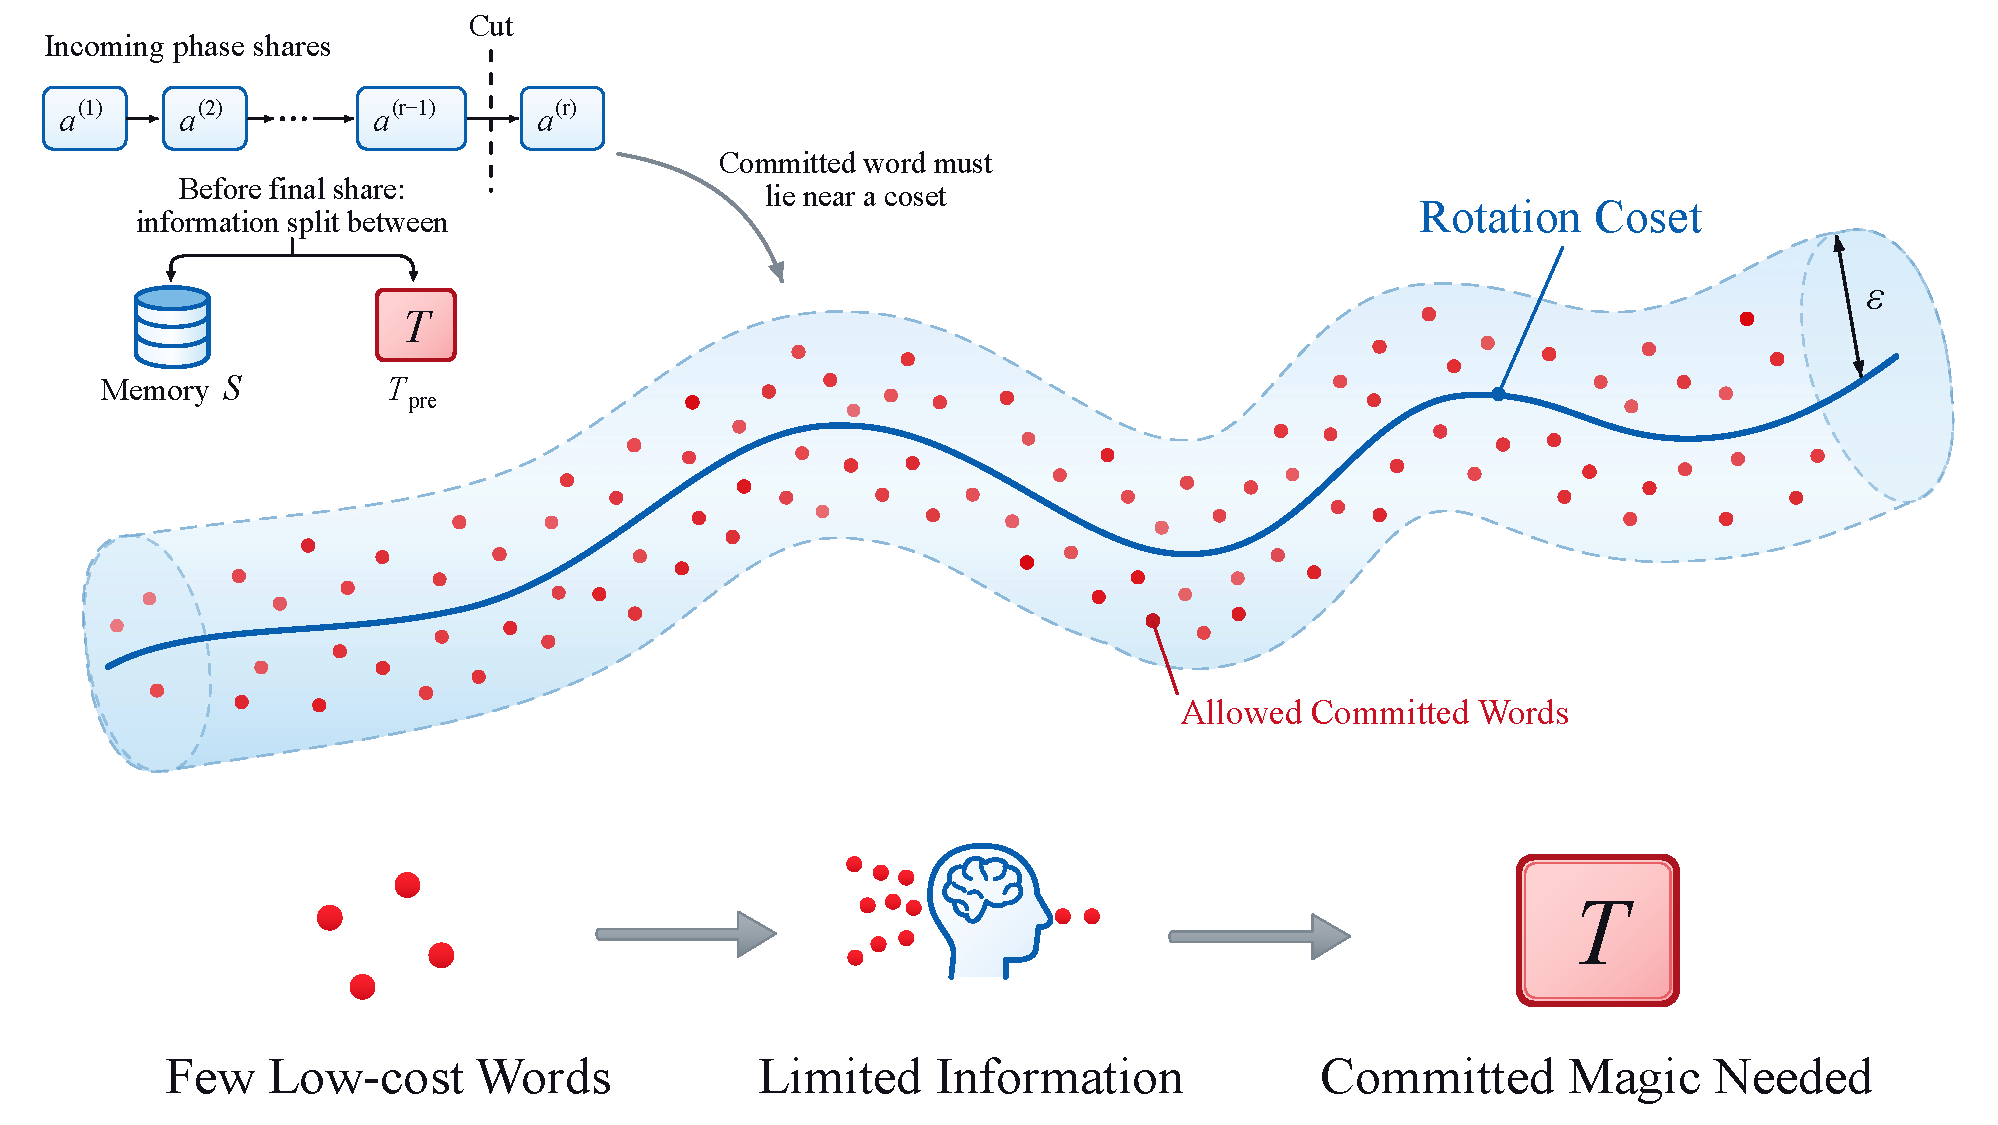
\includegraphics[width=0.92\textwidth]{fig0_schematic.pdf}
\caption{Origin of the per-bit committed-magic cost (schematic, not to scale). Top left: the shares $a^{(1)},\dots,a^{(r)}$ of a phase arrive in rounds. At the final inter-round cut, before the last share arrives, the information about the aggregate is split between the snapshot of size $S$ retained in memory and the $T$ gates $\Tpre$ already committed. Center: a committed word must lie within $\varepsilon$ of a rotation coset $G_1R_z(\theta)G_2$, a curve (blue) of codimension $\beta=2$ in $\SU$, and the tube of radius $\varepsilon$ around it contains few Clifford+$T$ words of low $T$-count (red). The tube contains at most $C_12^k\varepsilon^2+C_2(k+1)2^{k/2}$ words of $T$-count $\le k$ (Theorem~\ref{thm:tube}). Bottom: the scarcity of low-cost words implies that a cheap committed word carries little information about its coordinate, so each bit not retained in memory incurs a cost in committed magic.}
\label{fig:schematic}
\end{figure*}

The memory quantity in this trade measures deferred decisions rather than storage capacity. A control processor has gigabytes of memory: at $m=10^4$ coordinates and $\log_2K=33$, the entire aggregate occupies $41$\,kB, compared with $10^6$ magic states on the quantum side of the trade. The snapshot size $S$ measures \emph{deferred decision}: how much of the computation a schedule postpones lowering into the instruction stream until later rounds are available. This deferral cost arises when the scheduler emits into an append-only stream with bounded lookahead, a constraint motivated by real-time control requirements~\cite{Caune,Fowler}, or when the shares are produced upstream with randomness that the compiler does not hold, as can happen when randomized-compiling twirls~\cite{WallmanEmerson} are drawn outside the compiler. The cost of early commitment depends on the commitment rather than the final target. Every lower bound below holds conditionally on any fixed aggregate, including the zero aggregate whose target unitary is the identity (Corollary~\ref{cor:identity}). Thus, a computation that cancels completely can still have committed $\Theta(m\log(1/\varepsilon))$ $T$ gates before the cancellation could be known.

Merging phases before synthesis is an established approach to quantum circuit optimization. Phase-polynomial resynthesis combines parity phases~\cite{AmyMaslovMosca,AmyMosca}, continuous-parameter optimizers merge rotations~\cite{Nam}, and the ZX-calculus identifies nonlocal phase cancellations~\cite{KissingerWetering}. Related tools include $\mathrm{t}|\mathrm{ket}\rangle$~\cite{Sivarajah}, the TODD compiler~\cite{HeyfronCampbell}, and recent multiproduct commutation rules for Pauli-based computation~\cite{Mori26}. These methods use the circuit information available to their optimization passes. We impose the additional restriction that later shares are unavailable while earlier output is irrevocable. Under this restriction, even a circuit that an offline optimizer reduces to the identity can have a costly committed prefix.

We study the \emph{committed magic} $\Tpre$: the number of $T$ gates irrevocably emitted before the final share arrives. If the execution interface applies each emitted segment by the next round boundary, this quantity also counts the $T$ gates executed, and the magic states consumed, before the final share. A consumer that buffers the entire output until the end consumes no magic states early, but the emitted records remain irrevocable and are the objects counted by our bounds. A process that retains every share in memory has $\Tpre=0$; a process with no retained information must encode the earlier shares in committed output. Our two principal results are unconditional within the ancilla-free coordinatewise Clifford+$T$ model of Sec.~\ref{sec:setting}. We state them here for processes with zero failure probability ($\delta=0$) at nonzero approximation error $\varepsilon$. For failure probability $\delta>0$, the information requirement $m\log_2K$ is replaced by $(1-2\delta)m\log_2K-2mh_2(\delta)$.
\begin{itemize}\setlength\itemsep{1pt}
\item \textbf{General processes} (Theorem~\ref{thm:rate52}). For every fixed $\alpha<\tfrac52$, a sufficiently accurate process must pay at least $\alpha$ committed $T$ gates in expectation per bit of aggregate information not retained, after a per-coordinate allowance. The resulting asymptotic lower bound is $\tfrac52-o(1)$, uniformly over the frames created by its committed words.
\item \textbf{Rotation-segmented processes} (Theorem~\ref{thm:rate3seg}). If each coordinate's entire committed segment in a round is within $\varepsilon$ of a Clifford-framed $z$-rotation $CR_z(\varphi)C'$, as in per-rotation pipelines, the leading exchange-rate lower bound is $3$, with a lower-order allowance per coordinate. Fractional passthrough attains $3+o(1)$ under the grid-mean synthesis hypothesis of Sec.~\ref{sec:frontier}. Thus the lower bound is unconditional within this restricted model, while its matching upper bound depends on that hypothesis.
\end{itemize}
A separate consequence concerns single-rotation synthesis itself. Almost every $z$-rotation requires at least $3L-O(L/\log L)$ $T$ gates, unconditionally (Corollary~\ref{cor:typical}). This establishes the leading-order lower bound for typical rotations discussed by Ross and Selinger~\cite[Sec.~8.3]{RossSelinger}; it does not establish their stronger conjecture for every nonexceptional angle with an additive constant. A bound for Haar-typical unitaries alone cannot give this result, because $z$-rotations form a measure-zero subset of the full group.

The route to the streaming bounds also gives useful finite-accuracy estimates. A rate-one bound follows from counting all Clifford+$T$ words (Theorem~\ref{thm:main1}). Counting only words near a rotation coset gives a rate-two bound with explicit constants (Theorems~\ref{thm:tube} and~\ref{thm:rate2}). At $\varepsilon=10^{-10}$ and $S=0$, its finite-accuracy refinement gives $1.14$ committed $T$ gates per bit, compared with a sampled construction cost of $3.11$ (Corollary~\ref{cor:finite}, Sec.~\ref{sec:num}). The determinant method strengthens the asymptotic bound to every rate below $\tfrac52$.

Under a uniform equidistribution conjecture, the rate-three lower bound extends to general processes (Conjecture~\ref{conj:equid}, Theorem~\ref{thm:main2}). Under the same conjecture, words of cost at most $(2-\nu)L$, for any fixed $\nu\in(0,2)$, carry only $o(L)$ bits about a coordinate. Enumeration supports the conjecture on the frames tested. Sec.~\ref{sec:models} examines how side information, probabilistic mixing and quantum workspace change the resource accounting.

Our synthesis benchmark is provided by the arithmetic theory of exact Clifford+$T$ representation~\cite{KMM13} and ancilla-free approximation of rotations~\cite{Selinger15,RossSelinger}. Measurements and ancillary workspace change this benchmark. Repeat-until-success synthesis~\cite{PaetznickSvore,BRS} and finite fallback protocols~\cite{PQF} reduce expected $T$-count. Fourier-state phase kickback implements rotations by quantum addition~\cite{JonesFourier,Gidney}. Ancilla-assisted synthesis trades quantum workspace for $T$ gates and can synthesize many rotations jointly~\cite{LKS,GKW}. Catalytic rotation protocols also reduce $T$-depth~\cite{Kim26}, a separate resource from the $T$-count charged here. Existing non-Clifford resource lower bounds address the cost of realizing a target transformation~\cite{BCHK}; our bounds charge output committed before that target is known, even when it is ultimately the identity.

The rates $2$ and $3$ arise from different counting estimates. A single-qubit Clifford+$T$ word of minimal $T$-count $t$ implements one of at most $36\cdot2^t$ distinct unitaries~\cite{MA08}. Taking the logarithm gives one bit per $T$ gate, up to a constant allowance: this is the rate-one bound. The stronger bounds use correctness to confine a committed word to a tube of radius $\varepsilon$ around a rotation coset, a curve of codimension $\beta=2$ in the three-dimensional group (Fig.~\ref{fig:schematic}). If the tube contains the volume-law population $\approx2^{\tau}\varepsilon^{\beta}$ at cost $\tau$, encoding $b$ bits requires $\tau\ge b+\beta L$. The word pays an entry fee of $\beta L$ gates and one gate per bit thereafter. For the $\approx L$ bits of a whole coordinate, this gives the leading rate $1+\beta=3$. A low-cost alphabet accounts for the first few bits; the rate statements include an allowance for them.

The spectral estimate adds a counting remainder of order $\operatorname{poly}(\tau)2^{\tau/2}$~\cite{LPS,LPSII,PS18}. In the relevant cost range this term dominates the volume contribution, leaving a certified alphabet whose logarithm grows as $\tau/2$ rather than $\tau-2L$. This yields the weaker rate two; Sec.~\ref{sec:tube} explains the information bound. The determinant method reduces that remainder and approaches $\tfrac52$, where its boxes have shrunk to $\varepsilon$-cubes. At Clifford-framed cosets, the arithmetic of the frame gives the volume law up to a subexponential factor and yields rate three for rotation-segmented processes.



\paragraph{Contributions and prior work.} Our earlier work~\cite{Paper1} established a bit-level bound, which Theorem~\ref{thm:main1} reproves using the Matsumoto--Amano count in place of Kraft's inequality. The new unconditional results are the explicit count near arbitrary rotation cosets (Theorem~\ref{thm:tube}), the general exchange-rate bounds $2$ and $\tfrac52$ (Theorems~\ref{thm:rate2} and~\ref{thm:rate52}), and the volume law at Clifford cosets (Theorem~\ref{thm:clifford}). The last result gives both the rotation-segmented rate three and the almost-all single-rotation lower bound (Theorem~\ref{thm:rate3seg}, Corollary~\ref{cor:typical}). Whole-group covering exponents~\cite{PS18}, Haar-typical gate-count bounds~\cite{SMA}, and Selinger's worst-case bound over angles~\cite[Thm.~30]{Selinger15} do not control how many cheap words lie near a prescribed rotation coset, which is what a streaming lower bound needs.

We are not aware of an earlier bound below the square-root barrier of the spectral method for points of this $S$-arithmetic quaternion lattice near an arbitrary rotation coset. For related results on points of spheres near planes and in caps see~\cite{BourgainRudnick}, for small-scale equidistribution of spherical lattice points see~\cite{HumphriesRadziwill}, and for optimal strong approximation see~\cite{BKS,Sardari}. The matching construction is conditional on the grid-mean synthesis hypothesis, and the extension of rate three to general processes is conditional on Conjecture~\ref{conj:equid}.

Sec.~\ref{sec:setting} defines the model, Sec.~\ref{sec:results} presents the results, Sec.~\ref{sec:num} describes the numerical evidence, and Sec.~\ref{sec:models} examines the dependence on the synthesis model. Sec.~\ref{sec:disc} discusses the implications. All proofs are in the appendices. Extended numerical evidence and the results of Sec.~\ref{sec:models} with their proofs are in the Supplemental Material~\cite{SM}.


\section{Setting}\label{sec:setting}

The basic example has two rounds: the compiler first receives a masked phase share and later receives the correction that determines the aggregate. It can retain the earlier share until the correction arrives, or commit a gate sequence that already encodes some of that share. We formalize the information carried between rounds before specifying the phase family.

\paragraph{Retained information and restart.} A one-pass compiler reads the rounds in order and may use arbitrary working memory within a round. At a cut $c$ between rounds, it retains a finite bit string $\sigma_c$. The \emph{restart property} requires all later output to be determined by this snapshot and the remaining input stream. Control state and any random-tape state needed after the cut are included in $\sigma_c$; earlier output cannot be read back as extra memory. Snapshots use a prefix-free serialization. We define
\begin{equation}\label{eq:memory}
B_{\mathrm{cut}}(c):=|\sigma_c|,\qquad
S:=\max_{\mathrm{input}}\E_\rho\max_cB_{\mathrm{cut}}(c).
\end{equation}
Thus $S$ is the worst-input expected maximum number of bits retained across a round boundary. This is the charged one-pass model of~\cite{Paper1}, stated formally in Definition~\ref{def:model}. Appendix~\ref{app:model} gives the serialization details, the projective-distance formula and the block compiler, with proofs; no other result of~\cite{Paper1} is needed here.

\paragraph{Family.} Fix a modulus $Q\ge3$, step $\Delta=2\pi/Q$, alphabet size $K=Q-1$, and $m$ $\F_2$-independent $Z$-characters $P_1,\dots,P_m$ on $n\ge m$ qubits; let $V$ be a fixed public Clifford with $VZ_jV^\dagger=P_j$. The coordinates are independent tensor factors in this common frame. Linearly dependent commuting Paulis, such as $Z_1,Z_2,Z_1Z_2$, do not constitute three coordinates, and $m=10^4$ coordinates require at least $10^4$ data qubits. The aggregate is $x\in[K]^m$, with $[K]=\{0,\dots,K-1\}$. We retain the $(Q-1)$-symbol aggregate subfamily of~\cite{Paper1} for consistency: it omits residue $Q-1$, while shares still range over all of $\Z_Q$. All $Q$ residues represent distinct grid rotations; omitting one changes the entropy by only $\log_2(Q/(Q-1))=O(1/Q)$ bits per coordinate. The target is
\begin{equation}
U_x=V\Big(\bigotimes_{j\le m}R_z(\Delta x_j)\otimes I\Big)V^\dagger,\qquad R_z(\theta)=e^{-i\theta Z/2}.
\end{equation}
An $r$-round dispersed stream consists of shares $a^{(1)},\dots,a^{(r)}\in\Z_Q^m$, read in round-major order, with $\sum_ta^{(t)}\equiv x\pmod Q$. The \emph{canonical sharing} $\mathcal D$ draws the first $r-1$ shares independently and uniformly from $\Z_Q^m$, then sets $a^{(r)}=x-\sum_{t<r}a^{(t)}$.

Accuracy is measured by the projective distance $\dproj(A,B)=\inf_\phi\|A-e^{i\phi}B\|$. We require $0<\varepsilon<\sin(\pi/(2Q))$, so distinct grid rotations are more than $2\varepsilon$ apart and nearest-grid decoding is unambiguous. The \emph{tuned modulus} $Q_\varepsilon:=\lfloor\pi/(2\arcsin(2\varepsilon))\rfloor$ gives separation at least $4\varepsilon$ and $\log_2K_\varepsilon=L+O(1)$ (Lemma~\ref{lem:tuned}), where throughout
\begin{equation}
L:=\log_2(1/\varepsilon).
\end{equation}

\paragraph{Output model.} The \emph{coordinatewise ancilla-free Clifford+$T$ model} (CW) describes per-rotation pipelines that hand each generator of the phase polynomial to a single-qubit synthesizer, without ancillas or cancellation across coordinates~\cite{RossSelinger,Paper1}. Its write-once output is a list of irrevocable records $(j,g)$ with $j\in[m]$ and $g\in\{H,S,T\}$. The implemented unitary is $V(\bigotimes_jW_j)V^\dagger$, where $W_j$ is the ordered product of gates recorded on coordinate $j$. The $T$-count is the number of $T$ records. An output is \emph{correct} when $\dproj(W_j,R_z(\Delta x_j))\le\varepsilon$ for every coordinate.

By Lemma~\ref{lem:loc}, total error at most $\varepsilon$ implies coordinatewise correctness, so the lower bounds also hold under the total-error criterion of~\cite{Paper1}. Coordinatewise error at most $\varepsilon$ guarantees total error at most $m\varepsilon$. To meet a total error budget $\varepsilon_{\mathrm{tot}}$, the share-by-share construction of Sec.~\ref{sec:frontier} can use $\varepsilon_{\mathrm{tot}}/(mr)$ per share.

\paragraph{Correctness and committed magic.} A process must be correct with probability at least $1-\delta$ on every aggregate and every valid stream, with $\delta<\tfrac12$. Here \emph{zero error} means $\delta=0$, namely certain correctness at approximation tolerance $\varepsilon$. Let $T_t$ count the $T$ records emitted in round $t$, $\Tpre:=\sum_{t<r}T_t$ the \emph{committed magic}, and $\Tout=\Tpre+T_r$ the total output cost. The bounds count irrevocably emitted records. They also count gates executed before the next cut when the execution interface applies each emitted segment by that cut; statements about early magic-state consumption assume this interface.

Bars denote expectation over the random tape, the canonical sharing and a uniform aggregate. We write $L_\delta(m,K):=(1-\delta)m\log_2K-h_2(\delta)$ for the information remaining after the failure allowance, and $\rho_m(\bar T):=m\log_2(e(1+\bar T/m))+\allowbreak2\log_2(1+\bar T)+1$. The latter is an encoding overhead for the total $T$-count and its distribution among coordinates (Lemma~\ref{lem:ent}).

\paragraph{A concrete instance.} Take $n=m$, $P_j=Z_j$ and $V=I$. An upstream party holds grid phases $x\in[K]^m$, sends a uniform mask $a^{(1)}\in\Z_Q^m$ in round~1, and sends the correction $a^{(2)}=x-a^{(1)}$ in round~2. The compiler sees these shares but cannot access the upstream state. The first share is independent of $x$, exactly as required by canonical sharing. The targets are grid angles, so no rounding is needed and the full tolerance $\varepsilon$ is available for synthesis.

Suppose the executor applies the first-round output before round~2. A back end that synthesizes each arriving share~\cite{RossSelinger}, or retains it and synthesizes the aggregate later, is a CW process and is rotation-segmented (Sec.~\ref{sec:seg}). Retaining a share costs $\lceil\log_2Q\rceil$ bits per coordinate. Synthesizing both shares to error $\varepsilon/2$ guarantees coordinate error at most $\varepsilon$.

For $\varepsilon=10^{-10}$ and $m=10^4$, retaining everything costs about $41$\,kB and commits no magic before the correction arrives. Synthesizing each share on arrival at nominal share tolerance $\varepsilon/2$ gives a sampled mean of $102.32$ committed $T$ gates per coordinate (Sec.~\ref{sec:num}). Every zero-failure CW process with $S=0$, however it chooses its output, commits at least $37.40$ per coordinate in expectation (Table~\ref{tab:numbers}).

This input family does not describe every feedback circuit. Sources whose later angles depend on measurement outcomes, or whose shares are nonuniform, enter the bounds through the conditional entropy of information unavailable to the compiler (Theorem~\ref{S:thm:side}, Corollary~\ref{S:cor:side}(d)).

Real-valued angles also require a quantization budget. Rounding to the tuned grid alone can cost $2\sin(\pi/(4Q_\varepsilon))\simeq2\varepsilon$ per share, exceeding the entire tolerance. A real-angle pipeline must therefore ensure, for every coordinate $j$,
\begin{equation}\label{eq:anglebudget}
\sum_{t=1}^r\left[2\sin\!\left(\frac{|\theta^{(t)}_j-\hat\theta^{(t)}_j|}{4}\right)+\varepsilon_{j,t}\right]\le\varepsilon.
\end{equation}
Here $\hat\theta^{(t)}_j$ is the quantized share, the angle difference is reduced modulo $2\pi$ to $[-\pi,\pi]$, and $\varepsilon_{j,t}$ is its synthesis error.


\section{Results}\label{sec:results}

Table~\ref{tab:results} separates the models and hypotheses from the availability of finite-accuracy constants. All proofs are in the appendices. Appendix~\ref{app:lemmas} collects the elementary lemmas used throughout; in particular, the Matsumoto--Amano count (Lemma~\ref{lem:MA}) yields the rate-one bound.

\begin{table*}[t]
\centering\footnotesize
\caption{Exchange-rate results for zero failure probability. Rates refer to leading coefficients after the stated per-coordinate allowances. The finite-accuracy column uses $\varepsilon=10^{-10}$, $m=10^4$ and $S=0$, with costs per coordinate per pre-final round; the synthesis benchmark uses nominal share tolerance $\varepsilon/2$ for $r=2$. The input (R) is a known theorem, whereas Conjecture~\ref{conj:equid} and the grid-mean synthesis hypothesis are unproved.}
\label{tab:results}
\setlength{\tabcolsep}{3pt}\raggedright
\begin{tabular}{@{}p{0.19\textwidth}p{0.27\textwidth}p{0.22\textwidth}p{0.25\textwidth}@{}}
\toprule
\raggedright Result & \raggedright Model or extra hypothesis & \raggedright Constants and allowances & \raggedright Finite-accuracy use\tabularnewline
\midrule
\raggedright Rate $1$, Thm.~\ref{thm:main1} & \raggedright General CW & \raggedright Explicit & \raggedright Lower bound $21.75$\tabularnewline[3pt]
\raggedright Rate $2$, Thm.~\ref{thm:rate2}, Cor.~\ref{cor:finite} & \raggedright General CW; known (R) & \raggedright Explicit & \raggedright $25.72$ as stated; $37.40$ after refinement\tabularnewline[3pt]
\raggedright Rate $\tfrac52$, Thm.~\ref{thm:rate52} & \raggedright General CW; no unproved hypothesis & \raggedright For each $\alpha<\tfrac52$; $L_0(\alpha)$ and additive constants not explicit & \raggedright No evaluated numerical bound\tabularnewline[3pt]
\raggedright Rate $3$, Thm.~\ref{thm:rate3seg} & \raggedright $\varepsilon$-rotation-segmented CW & \raggedright Remainder $O(L/\log L)$; worst-case divisor estimate & \raggedright Current bound is vacuous\tabularnewline[3pt]
\raggedright Rate $3$, Thm.~\ref{thm:main2} & \raggedright General CW; Conj.~\ref{conj:equid} & \raggedright For each $\alpha<3$; constants not explicit & \raggedright No evaluated numerical bound\tabularnewline[3pt]
\raggedright Achievable rate $3$, Thm.~\ref{thm:frontier} & \raggedright Fractional passthrough; grid-mean hypothesis for the limiting rate & \raggedright Construction explicit; mean synthesis cost supplied separately & \raggedright Sampled mean $102.32$\tabularnewline
\bottomrule
\end{tabular}
\end{table*}

\subsection{Committed magic}\label{sec:main1}

\begin{theorem}[Committed magic]\label{thm:main1}
For every process as in Sec.~\ref{sec:setting} and every round $t\in[r-1]$,
\begin{equation}\label{eq:main1}
S+\bar T_t+m\log_236+\rho_m(\bar T_t)\ \ge\ L_\delta(m,K).
\end{equation}
Consequently
\begin{multline}
\bar\Tpre\ \ge\ (r-1)\big[L_\delta(m,K)-S-m\log_236\big]\\-(r-1)\,\rho_m\!\Big(\frac{\bar\Tpre}{r-1}\Big),
\end{multline}
and for the tuned family and $\delta=0$, $\bar\Tpre\ge(r-1)(m\log_2K_\varepsilon-S)-O(rm\log\log(1/\varepsilon))$.
\end{theorem}
Theorem~\ref{thm:main1} recovers the bit-level theorem of~\cite{Paper1} using Lemma~\ref{lem:MA} in place of Kraft's inequality. Its leading cost is one committed $T$ gate per bit not retained, per round, after the displayed allowances (Appendix~\ref{app:main1}). The constant $m\log_236$ comes from the finite choices in the single-coordinate normal-form count; $\rho_m$ accounts for the cost distribution among coordinates. These bounds do not depend on the target.

\begin{corollary}[Commitment before cancellation is knowable]\label{cor:identity}
Under the canonical sharing $\mathcal D$ the rounds $a^{(1)},\dots,a^{(r-1)}$ are i.i.d.\ uniform and independent of the aggregate $x$, and $\Tpre$ is a function of $(a^{(1)},\dots,a^{(r-1)},\rho)$ alone. Hence for every fixed aggregate $x\in[K]^m$,
\[
\E\big[\Tpre\,\big|\,X=x\big]=\bar\Tpre ,
\]
and the lower bounds of Theorems~\ref{thm:main1}, \ref{thm:rate2}, \ref{thm:rate52}, \ref{thm:rate3seg} and~\ref{thm:main2}, and those of Theorems~\ref{thm:rate115} and~\ref{thm:rate177} in Appendix~\ref{app:beyond}, hold after conditioning on $X=0$, for which $U_x=I$. A process that is required to be correct on every valid stream, and is not promised in advance that the aggregate vanishes, commits the same expected magic whether or not the phases cancel.
\end{corollary}
The corollary follows from the sharing distribution and is not an independent strengthening. A compiler given the promise $X=0$ can emit nothing. The statement concerns the resources that a universally correct process has already committed on a stream that turns out to cancel.

\subsection{Words near rotation cosets: the rate two}\label{sec:tube}

Single-qubit Clifford+$T$ modulo phase is an $S$-arithmetic group $\Gamma$ acting on the $3$-regular Bruhat--Tits tree, with $T$-count equal to tree distance~\cite{KMM13,PS18}. We write $\Lambda_k\subset\Gamma$ for the ball of $T$-count $\le k$ and (R) for the Ramanujan bound $\|T_j\|\le(j+1)2^{j/2}$ on the Hecke operators of this lattice~\cite{LPS,PS18}, which is a theorem (Appendix~\ref{app:tube}).


\begin{theorem}[Tube bound]\label{thm:tube}
For all $G_1,G_2\in\SU$, all $\varepsilon\in(0,1/8]$ and all $k\ge0$, with
$T_\varepsilon(C):=\{W:\exists\theta,\ \dproj(W,G_1R_z(\theta)G_2)\le\varepsilon\}$,
\begin{equation}\label{eq:tube}
\#\big(\Lambda_k\cap T_\varepsilon(C)\big)\ \le\ C_1\,2^k\varepsilon^2+C_2\,(k+1)\,2^{k/2},
\end{equation}
with the absolute constants $C_1=72\cdot4\sqrt2\le408$ and $C_2=24(1-2^{-1/2})^{-1}2^{3/2}\le232$.
\end{theorem}
The proof (Appendix~\ref{app:tube}) reduces the tube to a spherical cap through a Hopf fibration whose fiber is the coset. It majorizes this cap by a Poisson kernel of width $2\varepsilon$, whose spherical-harmonic coefficients are $r^\ell$ with $1-r=2\varepsilon$, allowing both constants to be determined explicitly. It then bounds the count by the Hecke operator through a rank-one sup-norm estimate.
The error term $(k+1)2^{k/2}$ cannot be reduced by this method, and it exceeds the main term in the whole range $k\le4L$ in which synthesized rotations live (Remark~\ref{rem:barrier}); Conjecture~\ref{conj:equid} below asks for an upper bound by the volume contribution plus a low-cost allowance, up to a subexponential factor.


\begin{theorem}[Rate two]\label{thm:rate2}
Under (R), put $n(\tau):=C_12^\tau\varepsilon^2+C_2(\tau+1)2^{\tau/2}$, $\tau_*:=\lceil2\log_2K\rceil$ and
\begin{equation}\label{eq:A2}
A_2:=1+\log_2 Z,\qquad Z:=\sum_{\tau\le\tau_*}n(\tau)2^{-\tau/2},
\end{equation}
so that $A_2=\log_2C_2+2\log_2(2\log_2K)+O(1)=O(\log\log(1/\varepsilon))$. Then for every round $t$,
\begin{equation}
\bar T_t\ \ge\ 2\big[(1-2\delta)m\log_2K-2m\,h_2(\delta)-S-mA_2\big],
\end{equation}
hence $\bar\Tpre\ge2(r-1)[(1-2\delta)m\log_2K-2mh_2(\delta)-S-mA_2]$.
\end{theorem}
Condition on the snapshot, the other rounds and correctness of a coordinate. These data fix the rotation coset near which its committed word must lie (Corollary~\ref{cor:profile}). In the relevant cost range, the counting remainder in Theorem~\ref{thm:tube} gives at most $\operatorname{poly}(\tau)2^{\tau/2}$ possible words of cost at most $\tau$. Taking a base-two logarithm bounds the information encoded by this truncated alphabet by $\tau/2+O(\log\tau)$. For variable costs, a cost-weighted entropy bound gives the corresponding conditional mutual-information bound in terms of the expected cost, $\bar\tau/2+A_2$ (Appendix~\ref{app:rate}). The information that the snapshot does not retain must be carried by these words, producing the factor two in Theorem~\ref{thm:rate2}. The square-root remainder limits the strength of this counting estimate.

The additive allowance matters at practical accuracies. At $\varepsilon=10^{-10}$, $A_2=20.0$ of the $32.9$ bits per coordinate, and the theorem as stated gives $25.72\,m$ committed $T$ gates per round at $S=0$. Corollary~\ref{cor:finite} sharpens this to $37.40\,m$ using the same assumptions and counting profile. It sums the cumulative counts directly, caps them by the total Clifford+$T$ count, and keeps the exact contribution of high-cost words. The two numbers are different evaluations of the same unconditional method.

\subsection{Beyond the square-root barrier: the rate five halves}\label{sec:rate52}

The square-root remainder of Theorem~\ref{thm:tube} limits the spectral method rather than the problem itself. A determinant method in the style of Bombieri--Pila and Heath-Brown~\cite{BombieriPila,HeathBrown}, adapted as in the cap lemmas of Bourgain--Rudnick~\cite{BourgainRudnick}, uses no automorphic input and no arithmetic property of the frame. The method lifts each word to its quaternion numerator, a lattice point on a sphere of radius $\asymp2^{t/4}$ in both real embeddings of $\Q(\sqrt2)$, cuts the tube into boxes, and proves that the affine determinant of any five points in a box vanishes. Thus, the points in each box lie on a round $2$-sphere. Using one determinant per box yields the rate $\tfrac{11}5$; splitting the sphere sections by the height of their hyperplane gives $\tfrac{17}7$; partitioning the numerators into fibers over rational planes and using projections, with the resulting case analysis checked exactly by an SMT solver on a continuum of box shapes, gives every rate below $\tfrac52$ (Appendices~\ref{app:beyond}--\ref{app:rate52}).


\begin{theorem}[Rate five halves]\label{thm:rate52}
For every $\alpha<\tfrac52$ there is $L_0(\alpha)$ such that, for every process as in Sec.~\ref{sec:setting}, every round $t<r$ and every $L\ge L_0(\alpha)$,
\begin{multline}\label{eq:rate52}
\bar T_t\ \ge\ \alpha\big[(1-2\delta)m\log_2K-2m\,h_2(\delta)\\-S-mA\big],\qquad A=O_\alpha(1).
\end{multline}
Behind it is the following tube bound. For every $0<\mu\le\tfrac1{10}$ there is $\eta_\mu(t)=o(t)$ such that, for all $G_1,G_2\in\SU$, all $\varepsilon\in(0,1/8]$ and all $t\le4(L+2)/(\tfrac85+\mu)$, with $C=G_1R_zG_2$,
\begin{equation}\label{eq:rate52tube}
\#\{W:\ t_{\min}(W)\le t,\ W\in T_\varepsilon(C)\}\ \le\ 2^{(\frac25-\frac\mu{11})t+\eta_\mu(t)}.
\end{equation}
\end{theorem}
Near the limiting rate, the exponent $\tfrac25-\tfrac\mu{11}$ is sharp for this case analysis, so the method approaches $\tfrac52$ but does not reach it. The obstruction is geometric: $\tfrac52$ is where its boxes shrink to $\varepsilon$-cubes, and a tube carrying words of $T$-count $(\tfrac52+o(1))L$ with gaps of at most $2^{o(L)}$ grid steps along its core would make $\tfrac52$ sharp (Proposition~\ref{prop:dense}). Theorem~\ref{thm:rate52} does not use (R) and holds uniformly over frames. This result concerns the asymptotic rate: its additive term and its $L_0(\alpha)$ are not explicit, and Theorem~\ref{thm:rate2} remains the bound we evaluate in Sec.~\ref{sec:num}.

\subsection{An achievable tradeoff family}\label{sec:frontier}


\begin{theorem}[Fractional passthrough]\label{thm:frontier}
For every $q\in\{0,\dots,m\}$ and every single-rotation synthesizer of cost $\tau(\varepsilon)$ per rotation to projective error $\varepsilon$, there is a deterministic zero-error one-pass CW process with
\begin{align}
S&\le\lceil q\log_2Q\rceil+O(\log(mQr)),\notag\\
T_t&\le(m-q)\,\tau(\varepsilon/r)\quad(t<r),\notag\\
\Tout&\le\big(m+(r-1)(m-q)\big)\,\tau(\varepsilon/r).
\end{align}
\end{theorem}
Under canonical sharing, every pre-final share is uniform on $\Z_Q$. The expected committed magic of fractional passthrough is therefore exactly $(r-1)(m-q)\bar\tau_Q(\varepsilon/r)$, where $\bar\tau_Q$ is the mean synthesis cost on that grid (Corollary~\ref{cor:frontier}).

\paragraph{Grid-mean synthesis hypothesis.}\label{hyp:gridmean} For fixed $r$ as $L\to\infty$, the matching asymptotic rate uses
\begin{equation}\label{eq:gridmean}
\bar\tau_{Q_\varepsilon}(\varepsilon/r)=(3+o(1))\log_2K_\varepsilon.
\end{equation}
Ross--Selinger synthesis motivates this hypothesis through its heuristic typical-angle cost~\cite{RossSelinger}; Sec.~\ref{sec:num} measures the grid mean at $\varepsilon=10^{-10}$. These observations support the hypothesis but do not prove it for the precision-dependent grids. Under~\eqref{eq:gridmean}, the passthrough family has leading slope three. Its first few released bits need not pay this slope: exact Clifford and $T$-power commitment can release them much more cheaply (Remark~\ref{rem:firstbit}, Sec.~\ref{sec:num}).

\subsection{Rotation-segmented processes: the rate three}\label{sec:seg}

For Clifford-framed cosets, the volume law holds up to a subexponential factor. In this case, the off-diagonal entry of a word is an arithmetic coordinate, and a divisor bound controls the remaining count.


\begin{theorem}[Volume law at Clifford cosets]\label{thm:clifford}
There is $\eta(\tau)=O(\tau/\log\tau)$ such that for all Cliffords $C_1,C_2$, all $\varepsilon\in(0,1/8]$ and all $\tau\ge1$, with $C=C_1R_zC_2$,
\begin{equation}\label{eq:clifford}
\#\{W:\ t_{\min}(W)\le\tau,\ W\in T_\varepsilon(C)\}\le2^{\eta(\tau)}\big(\tau+1+\varepsilon^22^\tau\big).
\end{equation}
For $G_1,G_2\in\Gamma$ with $t_{\min}(G_1)+t_{\min}(G_2)\le h$ the same holds with $\tau$ replaced by $\tau+h$.
\end{theorem}
\begin{corollary}[Typical $z$-rotations need $3L$]\label{cor:typical}
For every $\varepsilon\in(0,1/8]$ and every $s\ge0$, the set of $\theta\in[0,4\pi)$ for which $R_z(\theta)$ has an $\varepsilon$-approximation of $T$-count $\le3L-s$ has measure $\le C\,2^{\eta(3L)}\big(L2^{-L}+2^{-s}\big)$. The same bound holds for the fraction of grid angles $2\pi d/Q$, $d\in\Z_Q$, for the tuned modulus $Q=Q_\varepsilon$ and for any modulus $Q\ge c'/\varepsilon$ with $\sin(\pi/(2Q))>\varepsilon$.
\end{corollary}
Thus, all but a vanishing fraction of $z$-rotations need at least $3L-O(L/\log L)$ $T$ gates. This is an unconditional, leading-order lower bound for almost every angle, towards the stronger conjecture of~\cite[Sec.~8.3, Conj.~1]{RossSelinger}. That conjecture concerns every nonexceptional angle and an additive constant. Consequently, an asymptotic improvement on the passthrough rate would require a better commitment strategy: improving single-rotation synthesis alone cannot lower its leading coefficient for typical angles.


Theorem~\ref{thm:clifford} also bounds the processes used by per-rotation pipelines. Call a CW process \emph{$\vartheta$-rotation-segmented} if, on every input and tape, for every coordinate $j$ and every round $t<r$, the unitary $\overline W^{(t)}_j$ of the segment it emits on $j$ in round $t$ is within $\vartheta$ of $C\,R_z(\varphi)\,C'$ for some angle $\varphi$ and some Cliffords $C,C'$. The condition applies to the entire segment emitted on a coordinate within a round; two separately synthesized rotations emitted on the same coordinate in the same round need not satisfy it. Per-rotation synthesis of each share is of this form, and so is the fractional-passthrough family of Theorem~\ref{thm:frontier}, with $\vartheta=\varepsilon/r$. The constraint applies to the committed word itself, so the frames of Corollary~\ref{cor:profile}, which are the source of the gap between Theorems~\ref{thm:rate52} and~\ref{thm:main2}, play no role.

\begin{theorem}[Rate three for rotation-segmented processes]\label{thm:rate3seg}
For every $\vartheta$-rotation-segmented process as in Sec.~\ref{sec:setting} with $\vartheta\le1/8$, and every round $t<r$,
\begin{multline}\label{eq:rate3seg}
\bar T_t\ \ge\ \alpha_\vartheta\big[(1-2\delta)m\log_2K-2m\,h_2(\delta)\\-S-mA_\vartheta\big],\qquad\alpha_\vartheta:=1+\frac{2\log_2(1/\vartheta)}{\log_2K},
\end{multline}
with $A_\vartheta=O(\Lambda/\log\Lambda)$, $\Lambda:=\alpha_\vartheta\log_2K$. In particular, a $\vartheta$-rotation-segmented process with $\vartheta\le\varepsilon$ is $\varepsilon$-rotation-segmented, and $\alpha_\varepsilon\ge3-O(1/L)$, so $\bar\Tpre\ge3(r-1)\big(m\log_2K-S-O(mL/\log L)\big)-O(\delta rmL)$.
\end{theorem}
Theorem~\ref{thm:rate3seg} matches the rate of the passthrough family: in the model where each committed piece is within $\varepsilon$ of a Clifford-framed $z$-rotation, the exchange rate is $3$ to leading order in $L$, with an unconditional lower bound and an upper bound under the synthesis hypothesis of Sec.~\ref{sec:frontier}. Like Theorem~\ref{thm:rate52}, this is an asymptotic result. Its additive term is controlled by the worst-case divisor bound and the bound is vacuous at $\varepsilon=10^{-10}$ (Appendix~\ref{app:clifford}). Improving on this rate requires committing words that are not near any Clifford-framed rotation and whose frames, created by the prefix and suffix, carry the rest of the information. Theorem~\ref{thm:rate52} bounds how much such frames can help, and Conjecture~\ref{conj:equid} asserts that they cannot help at all.

\subsection{Rate three under an equidistribution conjecture}\label{sec:conj}


\begin{conjecture}[Volume law for every frame]\label{conj:equid}
There is a function $\psi(\tau)=o(\tau)$ such that for all $G_1,G_2\in\SU$, all $\varepsilon\in(0,1/8]$ and all $\tau\ge0$, with $C=G_1R_zG_2$,
\begin{equation}\label{eq:conj}
\#\{W:\ t_{\min}(W)\le\tau,\ W\in T_\varepsilon(C)\}\ \le\ 2^{\psi(\tau)}\big(1+2^\tau\varepsilon^{\beta}\big).
\end{equation}
\end{conjecture}
The exponent $\beta=2$ is the codimension of a rotation coset in the three-dimensional group. At Clifford cosets the conjecture is Theorem~\ref{thm:clifford}, with $2^{\psi(\tau)}=(\tau+1)2^{\eta(\tau)}=2^{O(\tau/\log\tau)}$. The conjecture asserts that no frame concentrates words more strongly than Clifford frames at exponential order. Theorem~\ref{thm:tube} gives $\tau/2+O(\log\tau)$ in place of $\psi(\tau)$ for every frame, and the determinant method lowers that exponent below $\tfrac25$ in the range $\tau\le(\tfrac52-o(1))L$.

Conjecture~1 of v2 of this manuscript~\cite{ExchangeV2} proposed a fixed-constant bound $c_0+c_1\tau+c\,2^\tau\varepsilon^2$ for grid hits. The growing additive term is necessary: Proposition~\ref{prop:cluster} rules out a bound with only $c_0+c\,2^\tau\varepsilon^2$. Even with a linear term, arithmetic orbits produce large steps in the count. For $(c_0,c_1)=(8,2)$, an enumerated cell near the identity requires $c\ge626.3$ at $\varepsilon=2.447978\times10^{-7}$ (Sec.~\ref{sec:num}). This excludes smaller choices of $c$ with those additive constants, but does not disprove the existence of every fixed triple. Heuristic arguments suggest unbounded requirements (Appendix~\ref{app:conj}). These observations motivate the present subexponential formulation, which also agrees with the proved Clifford-frame volume law.


\begin{theorem}[Rate three under Conjecture~\ref{conj:equid}]\label{thm:main2}
Assume Conjecture~\ref{conj:equid}, with $\psi$ non-decreasing, as one may take it. For every $\alpha<3$ there is $A_\alpha$, depending only on $\alpha$ and $\psi$, such that for every process as in Sec.~\ref{sec:setting} and every round $t<r$,
\begin{equation}\label{eq:rate3}
\bar T_t\ \ge\ \alpha\big[(1-2\delta)m\log_2K-2m\,h_2(\delta)-S-mA_\alpha\big].
\end{equation}
Moreover, for every $\nu\in(0,2)$, writing $D_t:=(1-2\delta)m\log_2K-2mh_2(\delta)-S$, $\tau_\nu:=\lfloor(2-\nu)L\rfloor$, and $\bar{\mathcal A}^{>}_t$ for the expected number of coordinates that are correct and whose word committed in round $t$ has minimal $T$-count greater than $\tau_\nu$,
\begin{equation}\label{eq:active}
\bar{\mathcal A}^{>}_t\ \ge\ \frac{D_t-m\,a_\nu}{\log_2K},\qquad a_\nu:=2+\psi(\tau_\nu)=o(L).
\end{equation}
\end{theorem}
Hence $\bar\Tpre\ge3(r-1)(m\log_2K-S)-o(rmL)$ for $\delta=0$. This additive form retains the per-coordinate allowance near the full-memory endpoint; a multiplicative rate comparison requires an information deficit of order $mL$. The structural consequence is quantization: a committed word of cost at most $(2-\nu)L$ carries at most $a_\nu=o(L)$ bits about its coordinate, and~\eqref{eq:active} counts how many coordinates per round must commit a word of cost above $(2-\nu)L$. Under the grid-mean synthesis hypothesis of Sec.~\ref{sec:frontier}, fractional passthrough, which commits whole coordinates, matches~\eqref{eq:rate3} to leading order. This matching construction does not establish that every optimal process commits whole coordinates. The finite-accuracy frontier also remains undetermined. Like Theorem~\ref{thm:rate52}, Theorem~\ref{thm:main2} concerns the asymptotic rate; its constants are not explicit (Appendix~\ref{app:conj}).


\section{Numerical evidence}\label{sec:num}

We enumerated all single-qubit Clifford+$T$ unitaries of $T$-count $\le22$ ($3.0\times10^8$ words) through the Matsumoto--Amano normal form. Details, two further tables and the scripts are in Sec.~\ref{S:sec:numsupp} of the Supplemental Material~\cite{SM}.

\paragraph{Counting exponents and prefactors (Fig.~\ref{fig:tube}).} We tested the identity coset and two Haar-random cosets at $\varepsilon\in\{2^{-4},\dots,2^{-8}\}$, with tuned moduli $Q_\varepsilon\in\{12,25,50,100,201\}$. A least-squares fit over the $136$ cells with count at least $30$ gives $\log_2N=1.001\,t-2.007\,L+\text{const}$, close to the exponents $(1,2)$ of Conjecture~\ref{conj:equid}. The prefactors are checked against the exact Haar prediction, rather than fitted: on the $30$ Haar-pair cells with expected count above $3000$, the ratios lie in $[0.98,1.04]$ for the grid and $[0.98,1.01]$ for the tube. Four arithmetic frames, built from Clifford+$T$ words of $T$-count $0$, $5$, $10$ and $15$, give the same exponents. These finite deterministic counts support the conjecture on the tested frames; they are not a statistical test of its uniform statement.

\paragraph{Arithmetic clustering and the conjecture.} Clifford cosets are isometric copies of the identity coset. Their count is suppressed below the onset $t\approx2L$ and can exceed the Haar prediction just above it, as whole arithmetic orbits enter the tube together. To probe these steps, we scan both dyadic accuracies and non-dyadic accuracies near orbit-entry thresholds. With $(c_0,c_1)=(8,2)$, the old fixed-constant form would require $c\ge53.5$ on the axis coset of $HT$ at $\varepsilon=2^{-5}$, $c\ge119.6$ on that coset at $\varepsilon=0.0265$, and $c\ge163.9$ on the identity coset at $\varepsilon=0.024532$.

An exact identity-coset enumeration reproduces the exhaustive counts and extends the scan over $\varepsilon\in(2^{-25},\tfrac18]$ and every modulus. Its largest requirement is $c\ge626.3$, at $\varepsilon=2.447978\times10^{-7}$, or $L\approx21.96$, with large requirements persisting across the scanned range. Further searches using shifted grids, orbits of least transverse norm up to $T$-count $300$, and algebraic families find no larger steps (Sec.~\ref{S:sec:numsupp}). These scans give lower bounds on any proposed constant; they do not establish that no finite constant exists.


\begin{figure*}[t]
\centering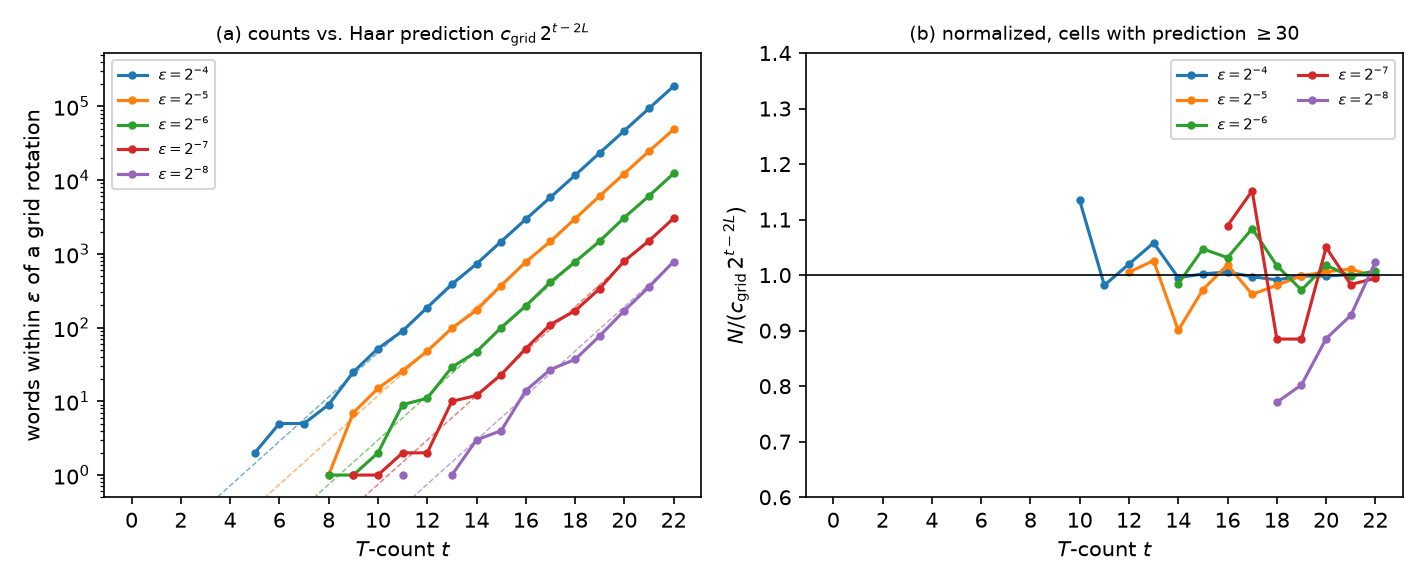
\includegraphics[width=0.92\textwidth]{fig1_tube_counts.png}
\caption{Number of Clifford+$T$ words of $T$-count exactly $t$ within $\varepsilon$ of a grid rotation on a Haar-random coset $G_1R_z(\theta)G_2$. (a) Counts (markers) compared with the exact Haar prediction $c_{\mathrm{grid}}2^{t-2L}$ with $c_{\mathrm{grid}}=48\varepsilon Q_\varepsilon/\pi$ (dashed). (b) The same counts divided by that prediction, plotted where the prediction is at least $30$. Every $\varepsilon$ has reached the Haar value by $t=22$. The exhaustive enumeration extends to $t=22$ ($3.0\times10^8$ words, $1.5\times10^8$ at $T$-count exactly $22$).}
\label{fig:tube}
\end{figure*}

\paragraph{Synthesis cost and the bounds (Fig.~\ref{fig:frontier}, Table~\ref{tab:numbers}).} For $L\le6$, enumeration gives the exact minimal $T$-count of every grid rotation. At share accuracy $\varepsilon/2$, as required by Theorem~\ref{thm:frontier} for $r=2$, the passthrough slopes are $3.333$ and $3.334$ at $L=5$ and $6$.

At $\varepsilon=10^{-10}$ we synthesize $20\,000$ uniform grid angles with Ross--Selinger synthesis in \texttt{pygridsynth}. We use $\varepsilon_{\mathrm{gs}}=2\eta$ for nominal projective tolerance $\eta$. The sampled means are $99.28$ at $\eta=\varepsilon$ ($3.020$ per bit) and $102.32$ at $\eta=\varepsilon/2$ ($3.113$ per bit). The library guarantees $\dproj\le\eta+O(\eta^3)$; the exact conversion and the parameter required for a strict tolerance are given in Sec.~\ref{S:sec:numsupp}. The $200$ re-synthesized validation angles in each benchmark satisfy the nominal tolerance. These sampled costs calibrate the construction; they do not certify all $20\,000$ words at its strict share budget.

Committing only the low $\ell$ bits of a share costs between $4.4$ and $20$ times the single-rotation slope per bit released, for the tested choices of $\ell$. These nonzero small-angle pieces still require a substantial synthesis cost. We call this the \emph{commitment threshold}: carrying substantial phase information can require a costly word even when few bits are released. The asymptotic statement for general frames depends on Conjecture~\ref{conj:equid}; the measured comparison concerns this particular partial-commitment strategy.

Table~\ref{tab:numbers} evaluates the rigorous bounds. At $S=0$, rate one gives $21.75\,m$ and the refined rate-two bound gives $37.40\,m$ committed $T$ gates per round. The basic rate-two statement gives $25.72\,m$ under the same assumptions. The sampled passthrough benchmark $102.32\,m$ at nominal share tolerance is a factor $2.74$ above the strongest evaluated lower bound. The refined rate-two bound exceeds rate one when $S<22.1\,m$ bits.

\paragraph{The first released bits.} The entry fee applies after a low-cost allowance. If $8\mid Q$, a share can be split into a nearest power of $T$ and a residual phase, using a fixed half-open convention at ties. Committing a Clifford releases two bits without a $T$ gate; allowing odd powers of $T$ releases a third bit for half a $T$ gate on average (Remark~\ref{rem:firstbit}). The star in Fig.~\ref{fig:frontier} uses $Q'=8\lfloor Q_\varepsilon/8\rfloor$ to meet this divisibility condition. The leading storage term for the residual is $\log_2(Q'/4)$ or $\log_2(Q'/8)$ bits per coordinate, respectively. For the per-coordinate abscissa $b:=B/m=\log_2(Q'-1)-S/m$, where the plot uses total $B=m\log_2K-S$, these points are therefore at $b=2-\log_2(Q'/(Q'-1))$ and $b=3-\log_2(Q'/(Q'-1))$. Changing the modulus also changes the aggregate entropy; the change is $O(2^{-L})$ bits per coordinate, quantified in the remark. These inexpensive first bits are consistent with the allowances in all exchange-rate bounds.


\begin{table}[t]
\centering\footnotesize
\caption{Finite-accuracy costs per coordinate per pre-final round at $\varepsilon=10^{-10}$, $m=10^4$, $\delta=0$ and $S=0$ ($L=33.22$, $Q_\varepsilon=7\,853\,981\,633$, $\log_2K=32.871$). ``Per bit'' divides the cost by $\log_2K$; ``coeff.'' is the leading coefficient of $-S$ (rate one's finite derivative is $0.94$). The refined rate-two row uses $(w,\lambda,n)=(2^{14},\tfrac5{16},40)$ in Corollary~\ref{cor:finite}; its coefficient is $1/\lambda=3.2$. With parameters optimized as $L\to\infty$, the leading coefficient tends to $2$. The numerical passthrough row uses nominal share tolerance $\eta=\varepsilon/2$ for $r=2$; calibration at $\eta=\varepsilon$ gives $99.28$. The strict error conversion is given in Sec.~\ref{S:sec:numsupp}.}
\label{tab:numbers}
\setlength{\tabcolsep}{4pt}\begin{tabular}{@{}l ccc@{}}
\toprule
& $\bar T_t/m$ & per bit & coeff.\\
\midrule
Thm.~\ref{thm:main1} (unconditional) & $21.75$ & $0.66$ & $1$\\
Thm.~\ref{thm:rate2}, Cor.~\ref{cor:finite} (known (R)) & $37.40$ & $1.14$ & $1/\lambda=3.2$\\
passthrough benchmark & $102.32$ & $3.11$ & $3.113$\\
\quad(\texttt{gridsynth}, nominal $\eta=\varepsilon/2$) & & &\\
\bottomrule
\end{tabular}
\end{table}

\begin{figure*}[t]
\centering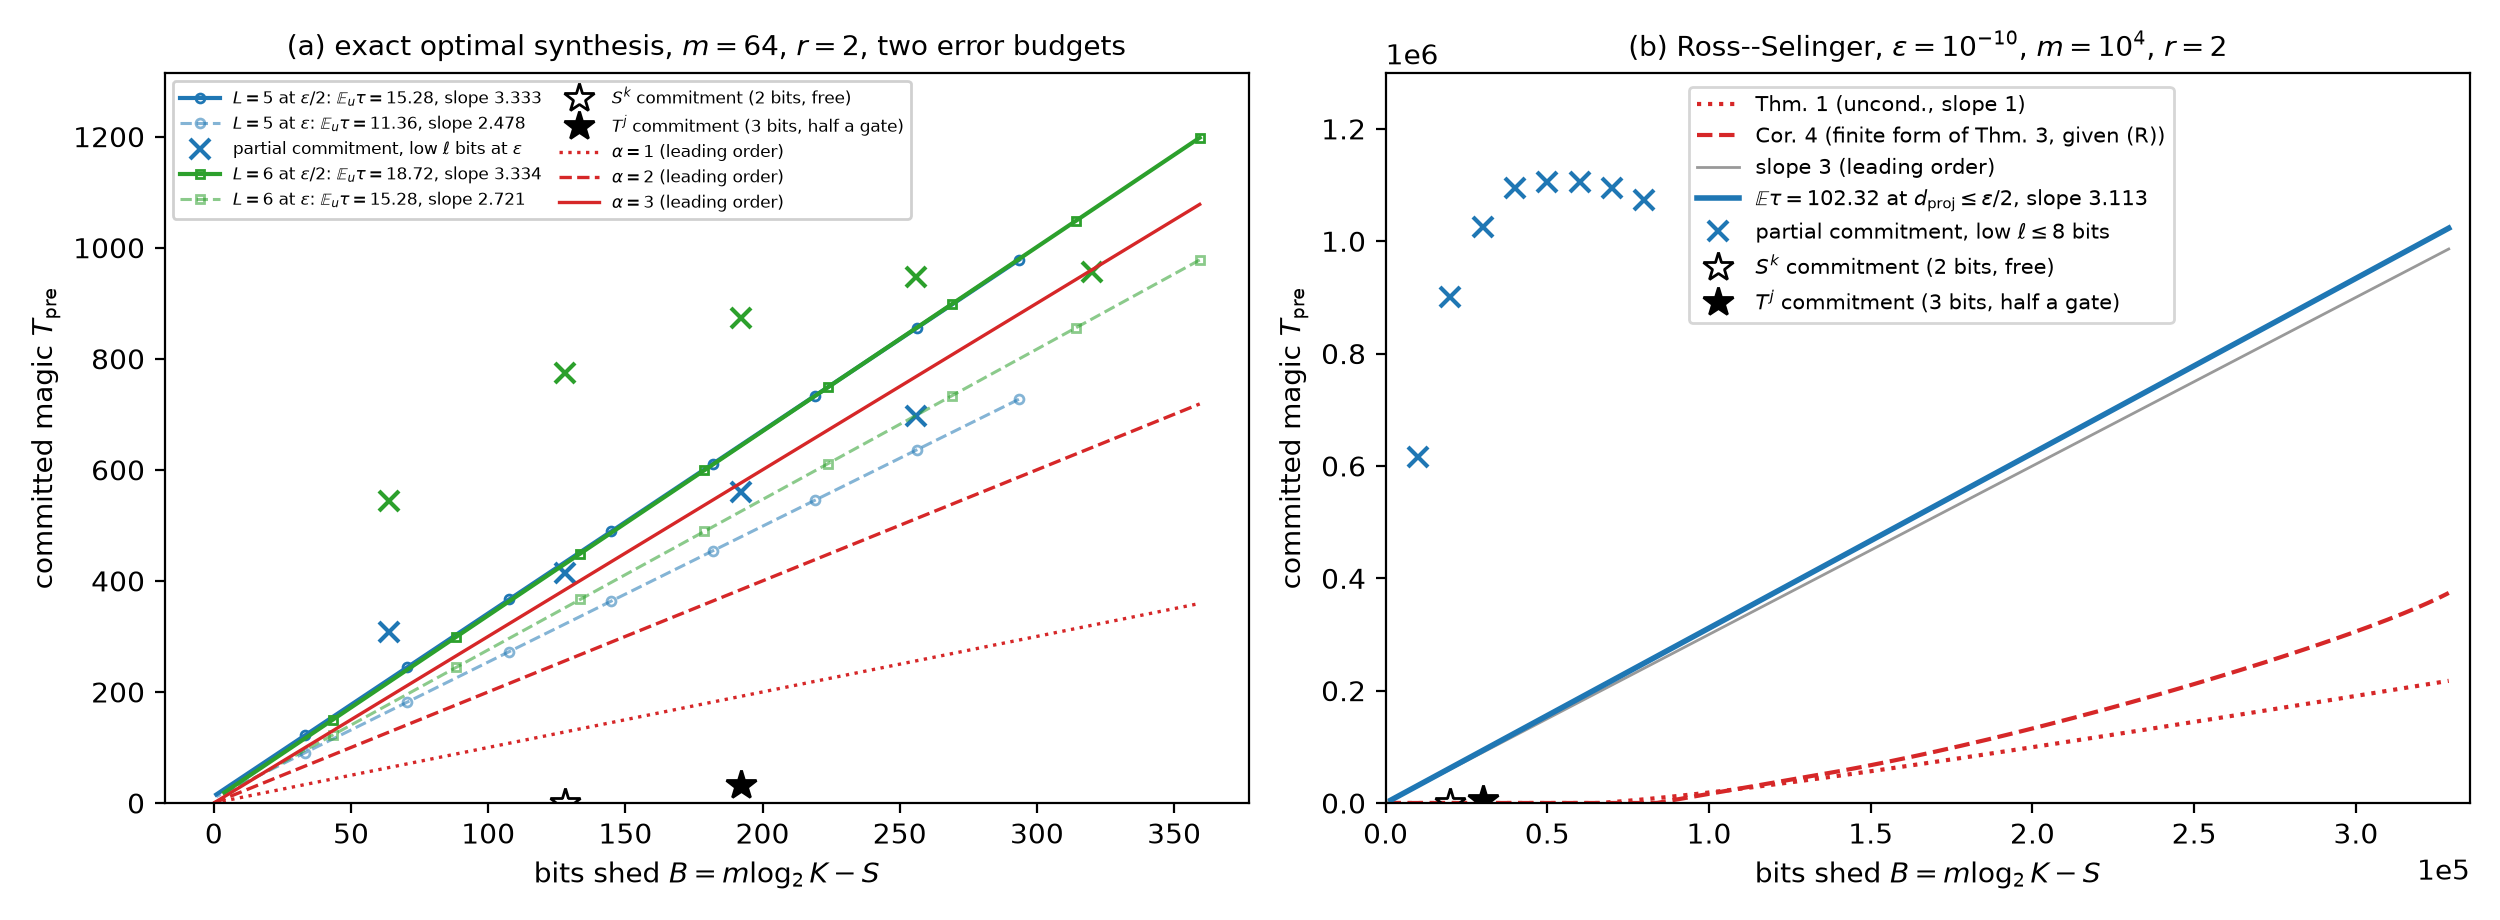
\includegraphics[width=0.92\textwidth]{fig2_frontier_twopanel.png}
\caption{Fractional passthrough and the lower bounds, for $r=2$. (a) Exact minimal synthesis costs at $L=5,6$, $m=64$. Solid curves use share error $\varepsilon/2$, certified by Theorem~\ref{thm:frontier}; dashed curves use word error $\varepsilon$ for single-rotation calibration. The lines of slope $1,2,3$ show only leading coefficients: the corresponding bounds are vacuous at these coarse accuracies. (b) At $\varepsilon=10^{-10}$ and $m=10^4$, the passthrough benchmark uses the sampled mean $102.32$ at nominal share tolerance $\varepsilon/2$, compared with the explicit lower bounds of Table~\ref{tab:numbers}. The rate-two curve optimizes Corollary~\ref{cor:finite} pointwise; the gray line shows slope three. Crosses commit only low share bits at word tolerance $\varepsilon$ (nominal in panel b). The star marks exact Clifford/$T$-power commitment: the first two bits per coordinate are free and a third costs half a $T$ gate on average. Its admissible modulus and the resulting abscissa correction are explained in Sec.~\ref{sec:num}.}
\label{fig:frontier}
\end{figure*}

\section{Beyond the coordinatewise model}\label{sec:models}

The lower bounds above apply to the CW model. Secs.~\ref{S:sec:side}--\ref{S:sec:mixing} of the Supplemental Material~\cite{SM} determine how they change in related models. Table~\ref{S:tab:models} there compares the rates. The main changes are summarized below.

\paragraph{Side information.} If the process can read side information $Y$ in every round without storing it, or the shares have any joint law with the aggregate, $m\log_2K$ in Theorem~\ref{thm:main1} is replaced by the conditional entropy $H(X\mid\mathrm{Past},\mathrm{Fut},Y)$ (Theorem~\ref{S:thm:side}). A process that can re-read the seed of a randomized-compiling twirl in every round has no information obstruction (a seed seen only before the cut has to be carried in the snapshot). A process that lacks an injective $\lambda$-bit seed independent of the aggregate is charged for at most $\lambda$ bits rather than $m\log_2K$. This specifies the precise scope of the ``randomize and lower late'' rule of~\cite{Paper1} (Corollary~\ref{S:cor:side}).

\paragraph{Probabilistic mixing.} Independently sampled coordinatewise mixed-unitary programs~\cite{Campbell17,Hastings17,KLMPP,Bothe} change the relevant phase resolution to an angular scale of order $\sqrt\varepsilon$. The bits needed to distinguish phases at this coarser resolution are the \emph{coarse bits}; their leading number is $\tfrac12L$ per coordinate. Known constructions can release the low $\tfrac12L-\tfrac12\log_2L-O(1)$ bits at bounded expected cost, while a positive cost per coarse bit remains. At $S=0$, the expected committed cost is at least $L-O(\log L)$ $T$ gates per coordinate per pre-final round, against $\tfrac32L$ achievable under the mixed-synthesis hypothesis (Theorem~\ref{S:thm:mixing}, Corollary~\ref{S:cor:mixstop}, Proposition~\ref{S:prop:mixach}). Under Conjecture~\ref{conj:equid}, the lower bound has leading coefficient three per coarse bit, with the fixed-$\nu$ threshold of Corollary~\ref{S:cor:mixq}. The mixed passthrough family matches its leading cost at $S=0$; the dependence on $S$ remains different. Quasi-probabilistic mixtures, whose resource is sample overhead, are outside this model.

\paragraph{Measurement adaptivity.} Repeat-until-success and fallback synthesis~\cite{PaetznickSvore,BRS,PQF} with $n-1$ ancillas retain a lower bound of order $L/n$ on the number of $T$ gates plus measurements per share not retained in memory (Proposition~\ref{S:prop:adaptive}).

\paragraph{Ancillas and batching.} Ancillas retained across a cut constitute memory and must be charged accordingly. The relevant model therefore uses clean ancillas. The construction uses phase-gradient addition~\cite{JonesFourier,Gidney} and ancilla-assisted lookup and diagonal synthesis~\cite{LKS,GKW}. With clean ancillas and a catalytic phase-gradient register prepared once, table lookups batched over $g\asymp\log L$ coordinates commit a share for $O(L/\log L)$ $T$ gates when $\log L=o(m)$ (Proposition~\ref{S:prop:batch}), so batching across coordinates eliminates any constant-rate law. At $\varepsilon=10^{-10}$ batching saves about $40\%$, rather than an order of magnitude. The constant-rate law thus applies to coordinatewise synthesis, which is what per-rotation pipelines implement.

\section{Discussion}\label{sec:disc}

For ancilla-free synthesis performed coordinate by coordinate, information not retained across a round boundary imposes a lower bound on expected committed magic. The explicit finite-accuracy inequalities have asymptotic exchange coefficient two. For every fixed $\alpha<\tfrac52$, a stronger unconditional bound applies at sufficiently high precision. Rotation-segmented processes have leading coefficient three, and fractional passthrough matches it under the grid-mean synthesis hypothesis~\eqref{eq:gridmean}. All these statements include per-coordinate allowances: $O(\log L)$ bits for rate two, a constant depending on $\alpha$ for each rate below $\tfrac52$, and $O(L/\log L)$ bits for the rotation-segmented rate three. They permit the inexpensive first bits illustrated in Sec.~\ref{sec:num}.

The rate of three follows from a volume count: a rotation coset has codimension $\beta=2$ in $\SU$, so a word pays $\beta L$ gates to enter the tube around it and one gate per bit thereafter. The spectral method yields a rate of two: the Ramanujan bound controls the tube only up to an error $2^{\tau/2}$, the square root of the number of all words of that cost. 

A rate of five halves is the exact limit of the determinant method with one auxiliary hyperplane per box, because $\tfrac52$ is where a box of the five-point determinant has shrunk to an $\varepsilon$-cube. Improving this rate requires showing that most $\varepsilon$-cubes along a tube are empty, and by Proposition~\ref{prop:dense} it requires at least excluding tubes that carry words of $T$-count $(\tfrac52+o(1))L$ with gaps of at most $2^{o(L)}$ grid steps along their core. 

Heuristically, arguments that cover a tube by balls cannot pass $\tfrac52$ (Sec.~\ref{S:sec:what52} of~\cite{SM}), and, to our knowledge, the standard square-root inputs---the Ramanujan bound, or a twisted Linnik conjecture of the kind that gives optimal strong approximation on $S^3$~\cite{BKS}---stop at rate $2$ in their natural circle-method and spectral implementations. 

Whether the true rate for general processes is $3$ remains open. Conjecture~\ref{conj:equid}, which the enumeration supports on Haar-random, arithmetic and Clifford cosets, asserts that the counting law is uniform across these frames.

These results have three implications. First, $S=0$ makes the information deficit largest. When angles are produced on the quantum side---qubitization, a QROM-loaded phase table, or adaptive QSVT phases---a classical snapshot of them may be unavailable. Our proof uses Fano's inequality for a classical stream and does not cover that setting; extending the resource accounting to quantum inputs is a direction for further work.

Second, the portions of memory that can be released cheaply depend on the synthesis mechanism. Under Conjecture~\ref{conj:equid}, a deterministic committed word of cost at most $(2-\nu)L$, for fixed $\nu>0$, carries only $o(L)$ bits (Theorem~\ref{thm:main2}). The partial-commitment strategy tested at $\varepsilon=10^{-10}$ costs $4.4$ to $20$ times the single-rotation slope per low bit released. Probabilistic mixing instead permits bounded-cost release of the low $\tfrac12L-\tfrac12\log_2L-O(1)$ bits~\cite{Bothe}; above this region, Corollary~\ref{S:cor:mixq} gives a commitment threshold under the same conjecture. The constructions that match the leading costs commit whole coordinates, but whether every optimal process must do so remains open.

Third, side information enters through a conditional entropy. Randomization raises the cost of commitment only to the extent that its seed is unavailable to the compiler after the cut.

Two unconditional statements provide complementary constraints on the arithmetic question: Selinger's worst-case $T$-count $4L-9$ for an $\varepsilon$-dependent angle~\cite[Thm.~30]{Selinger15}, and the covering exponents of Parzanchevski and Sarnak, who show that some single-qubit unitaries need $T$-count $4L$ while all are reachable at $6L$~\cite{PS18}. The committed-magic frontier concerns typical rather than worst-case behavior and similarly lies between rigorous and conjectural covering exponents. Closing the gap between $\tfrac52$ and $1+\beta$ for committed words with arbitrary frames remains an open problem.


\begin{acknowledgments}
J.Y. thanks Ke Lin of Xidian University and members of Yangyang Li's group
for their guidance and support.

Y.L. acknowledges support from the National Natural Science Foundation of
China under Grant No.~62476209, the Key Research and Development Program of
Shaanxi under Grant No.~2024CY2-GJHX-18, and the Fundamental Research Funds
for the Central Universities under Grant No.~QTZX26097. X.-H.D.
acknowledges support from the Science, Technology and Innovation Commission of Shenzhen
Municipality (Grant Nos.~JCYJ20170412152620376 and KYTDPT20181011104202253),
the Innovation Program for Quantum Science and Technology (Grant
No.~2021ZD0301703), the Guangdong Major Project of Basic Research (Grant
No.~2025B0303000007), and the Shenzhen Science and Technology Program
(Grant No.~KQTD20200820113010023).

Generative AI tools assisted with manuscript preparation, literature discovery,
code and repository maintenance, and consistency checks. The authors
independently reviewed the generated text, citations, code, and numerical claims
and take full responsibility for this work. AI output was not used as a
scientific source or as independent proof verification.
\end{acknowledgments}

\section*{Author contributions}
J.Y. developed the theory and proofs, implemented the enumeration, synthesis and certificate code, and performed the numerical computations and analyses. Y.L. and X.-H.D. supervised the research. Y.L. reviewed and revised the manuscript, and provided project administration and funding support. H.L. contributed to data visualization and helped compile the literature and organize the numerical data. X.-H.D. independently validated the theoretical derivations, numerical results, and computational artifacts. All authors contributed to writing the manuscript, discussed the results, and approved the final version.

\section*{Data availability}
{\raggedright
Updated code, numerical data, and computational certificates supporting this work
will be made available at \url{https://github.com/OIerYangJZ/memory-magic-exchange-law}.\par}


\appendix

\section{The streaming model}\label{app:model}

This appendix records the formal streaming definitions used in Sec.~\ref{sec:setting} and proves the projective-distance and block-compiler statements. The definitions follow~\cite[Defs.~9, 13, 20, 21]{Paper1}; the two statements are~\cite[Lem.~1, Prop.~10]{Paper1}. Together they make the present paper self-contained.

\begin{definition}[Charged one-pass process]\label{def:model}
A \emph{charged one-pass process} on the stream $a^{(1)},\dots,a^{(r)}$ is an algorithm with a random tape $\rho$ and a write-once output tape such that
\begin{enumerate}\setlength\itemsep{0pt}
\item[(i)] it reads the stream once, in order, and may keep unbounded internal state while reading a round;
\item[(ii)] at each \emph{cut} $c$ between consecutive rounds it emits a \emph{snapshot} $\sigma_c$, a finite bit string, with the \emph{restart} property: everything the process writes after $c$ is a function of $\sigma_c$ and of the part of the stream after $c$. The tape $\rho$ is part of $\sigma_c$, so a process that wishes to reuse its randomness pays for it;
\item[(iii)] snapshots are serialized in a prefix-free code, whence $H(\sigma_c)\le\E|\sigma_c|$;
\item[(iv)] its \emph{charge} is $S:=\max_{\mathrm{input}}\E_\rho\max_cB_{\mathrm{cut}}(c)$, where $B_{\mathrm{cut}}(c):=|\sigma_c|$.
\end{enumerate}
For $p>1$ passes the process may re-read the stream $p$ times, and the object playing the role of $\sigma_c$ is the transcript of all $2p-1$ crossings of the cut.
\end{definition}
Condition (iii) can be enforced with negligible overhead: prefixing a snapshot with its own length using Elias-$\gamma$ coding makes any serialization prefix-free at a cost of $2\log_2(|\sigma_c|+1)+1$ bits, which is dominated by the $O(\log(mQr))$ terms of every construction below. Condition (ii) is the substantive restriction imposed by an append-only instruction stream: the process cannot revise its earlier output, and any information needed later must be retained in the snapshot.

\begin{definition}[Dispersed family, canonical sharing, tuned modulus]\label{def:family}
With the family of Sec.~\ref{sec:setting}, a dispersed stream is any $a^{(1)},\dots,a^{(r)}\in\Z_Q^m$ with $\sum_ta^{(t)}\equiv x\pmod Q$. Correctness is required on every such stream. The canonical sharing $\mathcal D$ and tuned modulus $Q_\varepsilon$ are those defined in Sec.~\ref{sec:setting}.
\end{definition}

\begin{lemma}[Tuned modulus]\label{lem:tuned}
For $0<\varepsilon\le1/8$ one has $Q_\varepsilon\ge6$, $\sin(\pi/(2Q_\varepsilon))\ge2\varepsilon$, and $\log_2K_\varepsilon=L-\log_2(4/\pi)+o(1)=L-0.35+o(1)$.
\end{lemma}
\begin{proof}
$Q_\varepsilon\le\pi/(2\arcsin(2\varepsilon))$ gives $\pi/(2Q_\varepsilon)\ge\arcsin(2\varepsilon)$, i.e.\ $\sin(\pi/(2Q_\varepsilon))\ge2\varepsilon$, which satisfies the accuracy condition of Sec.~\ref{sec:setting} with a factor $2$ to spare. $\varepsilon\le1/8$ gives $\arcsin(2\varepsilon)\le\arcsin\tfrac14<\pi/12$ and hence $Q_\varepsilon\ge6$. Since $\arcsin(2\varepsilon)=2\varepsilon(1+O(\varepsilon^2))$, $Q_\varepsilon=\pi/(4\varepsilon)+O(1)$ and $\log_2K_\varepsilon=\log_2(Q_\varepsilon-1)=L+\log_2(\pi/4)+o(1)$.
\end{proof}

\begin{lemma}[Projective distance]\label{lem:dproj}
For unitaries $A,B$ of equal size, $\dproj(A,B)=2\sin(\Theta/4)$, where $\Theta\in[0,2\pi]$ is the length of the shortest closed arc of the unit circle containing $\spec(B^\dagger A)$.
\end{lemma}
\begin{proof}
By unitary invariance of the operator norm,
\[\dproj(A,B)=\inf_\phi\|B^\dagger A-e^{i\phi}I\|=\inf_\phi\max_{\lambda\in\spec(B^\dagger A)}|\lambda-e^{i\phi}|,\]
since $B^\dagger A$ is normal. Write $d(\phi,\lambda)\in[0,\pi]$ for angular distance, so that $|\lambda-e^{i\phi}|=2\sin(d(\phi,\lambda)/2)$, increasing in $d$. If $e^{i\phi_0}$ is the midpoint of a shortest arc, every eigenvalue is within $\Theta/2$ of it and the endpoints attain this distance, so the maximum equals $2\sin(\Theta/4)$. Conversely, for any $\phi$ put $D:=\max_\lambda d(\phi,\lambda)\le\pi$; the spectrum then lies in the closed arc of length $2D$ centered at $e^{i\phi}$, so $\Theta\le2D$ by minimality, and $\max_\lambda|\lambda-e^{i\phi}|=2\sin(D/2)\ge2\sin(\Theta/4)$.
\end{proof}

\begin{proposition}[Block compiler]\label{prop:block}
For every $q\le m$ there is a deterministic one-pass process which, on every $r$-round dispersed stream, keeps the running sums modulo $Q$ of $q$ designated coordinates in a snapshot of at most $\lceil q\log_2Q\rceil+O(\log(mQr))$ bits and, at round $r$, knows the exact aggregate $x_j$ of each designated coordinate.
\end{proposition}
\begin{proof}
The state carried across a cut is the vector of partial sums in $\Z_Q^q$, encoded as one integer in $[Q^q]$, i.e.\ $\lceil q\log_2Q\rceil$ bits. The remainder of the snapshot stores the round index, the position within the round and a fixed-size program counter, using $O(\log(mQr))$ bits, made prefix-free as in Definition~\ref{def:model}\,(iii). The designated set is fixed in advance and need not be stored. Each arriving share is added modulo $Q$ into its partial sum, so after round $r$ the $j$-th sum is $\sum_ta^{(t)}_j\bmod Q=x_j$.
\end{proof}
The gap between $\log_2Q$ here and the $\log_2K$ of the lower bounds is the difference between storing a share, which ranges over $\Z_Q$, and the entropy of an aggregate, which ranges over $[K]$; it is $\log_2(Q/K)=O(1/Q)$ per stored coordinate.

\section{Lemmas}\label{app:lemmas}


\begin{lemma}[Localization]\label{lem:loc}
For unitaries $A=\bigotimes_jA_j$, $B=\bigotimes_jB_j$ on the same tensor factors,
\[\max_j\dproj(A_j,B_j)\le\dproj(A,B)\le\sum_j\dproj(A_j,B_j).\]
For $2\times2$ unitaries, $\dproj(A,B)=\sqrt{2-|\tr(B^\dagger A)|}$.
\end{lemma}

\begin{lemma}[Matsumoto--Amano count]\label{lem:MA}
The number of single-qubit Clifford+$T$ unitaries modulo phase of minimal $T$-count exactly $t$ is $n_1(0)=24$ and $n_1(t)=36\cdot2^t$ for $t\ge1$; hence $\sum_{s\le t}n_1(s)=72\cdot2^t-48$, and the number of $m$-tuples with total minimal $T$-count at most $T$ is $N^{\le}_m(T)\le36^m2^T\binom{T+m}{m}$.
\end{lemma}

\begin{lemma}[Entropy versus $T$-count]\label{lem:ent}
Let $M=(\overline W_1,\allowbreak\dots,\allowbreak\overline W_m)$ be a random $m$-tuple of single-qubit Clifford+$T$ unitaries and $T\ge\sum_jt_{\min}(\overline W_j)$ a random integer. Then $H(M)\le\bar T+m\log_236+\rho_m(\bar T)$.
\end{lemma}

\begin{lemma}[Identity coset]\label{lem:identity}
If $2\varepsilon^24^k<1$, i.e.\ $k<L-\tfrac12$, the only Clifford+$T$ unitaries with denominator exponent $\le k$ within $\varepsilon$ of some $R_z(\theta)$ are the eight powers of $T$.
\end{lemma}
Lemma~\ref{lem:MA} is the source of the exchange rate: a $T$ gate carries at most $\log_22=1$ bit. Lemma~\ref{lem:identity} is an elementary instance of the entry fee (Appendix~\ref{app:conj}).


\begin{proof}[Proof of Lemma~\ref{lem:loc}]
By Lemma~\ref{lem:dproj}, $\dproj(A,B)=2\sin(\Theta/4)$ where $\Theta\in[0,2\pi]$ is the length of the shortest closed arc containing $\spec(B^\dagger A)$. The spectrum of $\bigotimes_jB_j^\dagger A_j$ consists of the products of eigenvalues. Fix $j$ and two eigenvalues $\lambda,\lambda'$ of $B_j^\dagger A_j$ at circular distance $\theta_j\le\pi$; multiplying both by a fixed product $\mu$ of eigenvalues of the other factors gives two points of the joint spectrum at circular distance $\theta_j$, and any closed arc containing both has length at least $\theta_j$. Hence $\Theta\ge\theta_j$, and since $\sin$ increases on $[0,\pi/2]$, $\dproj(A,B)\ge2\sin(\theta_j/4)=\dproj(A_j,B_j)$. For the right inequality replace one factor at a time: $\|\bigotimes A_j-e^{i\sum\phi_j}\bigotimes B_j\|\le\sum_j\|A_j-e^{i\phi_j}B_j\|$, then take infima. For the closed form, with eigenphases $a,b$ of $B^\dagger A$ one has $|\tr|^2=2+2\cos\Theta$ and $2\sin(\Theta/4)=\sqrt{2-2\cos(\Theta/2)}=\sqrt{2-|\tr|}$, using $\cos(\Theta/2)\ge0$ for $\Theta\le\pi$.
\end{proof}

\begin{proof}[Proof of Lemma~\ref{lem:MA}]
Every Clifford+$T$ unitary has a unique normal form $(T|\epsilon)(HT|SHT)^*C$ with $C$ one of the $24$ Cliffords modulo phase~\cite{MA08}, and the normal form is $T$-optimal~\cite{KMM13}. The number of strings with exactly $t$ occurrences of $T$ is $2^{t-1}$ (initial $T$ present) plus $2^t$ (absent), multiplied by $24$. For tuples, $\prod_jn_1(t_j)\le36^m2^{\sum_jt_j}$ and the number of $(t_j)$ with $\sum t_j\le T$ is $\binom{T+m}{m}$.
\end{proof}

\begin{proof}[Proof of Lemma~\ref{lem:ent}]
Encode $M$ by the Elias-$\gamma$ code of $T$ (at most $2\log_2(T+1)+1$ bits) followed by an index among $N^{\le}_m(T)$ tuples; $H(M)$ is at most the expected length of this prefix code. Use $\log_2\binom{T+m}{m}\le m\log_2(e(1+T/m))$, which is concave in $T$, and apply Jensen's inequality.
\end{proof}

\begin{proof}[Proof of Lemma~\ref{lem:identity}]
Write the unitary as
\[2^{-k/2}\begin{pmatrix}u&-t^\dagger\omega^l\\ t&u^\dagger\omega^l\end{pmatrix}\]
with $u,t\in\Z[\omega]$, $\omega=e^{i\pi/4}$, $uu^\dagger+tt^\dagger=2^k$~\cite{KMM13}. By the closed form of Lemma~\ref{lem:loc}, closeness to a diagonal unitary forces $|t|^2\le2\varepsilon^22^k$. The Galois conjugate $\sqrt2\mapsto-\sqrt2$ of the norm equation gives $|t^\bullet|^2\le2^k$. Hence $\xi:=tt^\dagger\in\Z[\sqrt2]$ is totally nonnegative with $N_{\Q(\sqrt2)/\Q}(\xi)=\xi\xi^\bullet\le2\varepsilon^24^k<1$, forcing $\xi=0$ and $t=0$. Then $uu^\dagger=2^k$; the prime above $2$ in $\Z[\omega]$ is $(1-\omega)$ with $(1-\omega)^4\sim2$, and the units of relative norm one are the $\omega^j$, so $u=\omega^j(1-\omega)^{2k}$ times a unit and the unitary is $\operatorname{diag}(\omega^a,\omega^b)$ modulo phase.
\end{proof}

\section{Proof of Theorem~\ref{thm:main1} and Corollary~\ref{cor:identity}}\label{app:main1}

\begin{proof}[Proof of Theorem~\ref{thm:main1}]
Fix $t$. Let $A:=a^{(t)}$, $\mathrm{Past}:=(a^{(s)})_{s<t}$, $\mathrm{Fut}:=(a^{(s)})_{s>t}$ (which includes round $r$), and $Z:=(\mathrm{Past},\mathrm{Fut},\rho)$.

\emph{(i) $H(A\mid Z)=m\log_2K$.} Under $\mathcal D$ the joint law of $(a^{(1..r-1)},x)$ is $Q^{-m(r-1)}P_X(x)$ with $a^{(r)}$ determined. Conditioning on $(\mathrm{Past},\mathrm{Fut})$ fixes $c:=\sum_{s\ne t}a^{(s)}$ and $x=A+c$, so the conditional law of $A$ is proportional to $P_X(A+c)$, i.e.\ uniform on the translate $[K]^m-c$. The tape is independent of the stream.

\emph{(ii) Message and Fano.} Let $M_t:=(\overline W^{(t)}_1,\dots,\overline W^{(t)}_m)$ be the tuple of unitaries (modulo phase) implemented by the gate segments emitted on the respective coordinates during round $t$, and $\sigma_t$ the restart snapshot at the cut after round $t$. Given $\rho$, the process is deterministic. The segments emitted before round $t$ are a function of $(\mathrm{Past},\rho)$, and those emitted after the cut are a function of $(\sigma_t,\mathrm{Fut})$ by the restart semantics of Definition~\ref{def:model}\,(ii). Hence the final unitary on coordinate $j$, $U^{<t}_j\overline W^{(t)}_jU^{>t}_j$, is a function of $(M_t,\sigma_t,Z)$. On success it is within $\varepsilon$ of $R_z(\Delta x_j)$, and nearest-grid decoding recovers $x_j$ because neighboring grid rotations are more than $2\varepsilon$ apart; thus $A=x-c$ is recovered with error probability $\le\delta$. Fano's inequality gives $H(A\mid M_t,\sigma_t,Z)\le h_2(\delta)+\delta\log_2(K^m-1)$, i.e.\ $I(A;M_t,\sigma_t\mid Z)\ge L_\delta(m,K)$.

\emph{(iii) Message size.} $I(A;M_t,\sigma_t\mid Z)\le H(\sigma_t)+H(M_t)$. The snapshot serialization is prefix-free (Definition~\ref{def:model}\,(iii)), so $H(\sigma_t)\le\E|\sigma_t|\le S$, because the worst-input expectation bounds the input average. The number $T_t$ of $T$ records emitted in round $t$ is at least $\sum_jt_{\min}(\overline W^{(t)}_j)$, so Lemma~\ref{lem:ent} gives $H(M_t)\le\bar T_t+m\log_236+\rho_m(\bar T_t)$. This proves~\eqref{eq:main1}. Summing over $t$ and using concavity of $\rho_m$ proves the rest.
\end{proof}

\begin{remark}[Multiple passes]
For $p$ forward passes, the alternating-simulation transcript---all $2p-1$ crossing snapshots together with the unitary tuple committed while scanning rounds $<r$ in any pass, cut between rounds $<r$ and round $r$ as in~\cite{Paper1}---determines the output, and the same argument gives $\Sigma_p+\bar T_A+m\log_236+\rho_m(\bar T_A)\ge L_\delta$ with $\Sigma_p\le(2p-1)S$. The decomposition by round, and hence the factor $r-1$, is a one-pass phenomenon: a process that rereads round $t$ after seeing round $r$ need not commit anything during round $t$.
\end{remark}

\begin{proof}[Proof of Corollary~\ref{cor:identity}]
Independence is item (i) of the proof of Theorem~\ref{thm:main1}; $\Tpre$ counts records emitted while reading rounds $<r$, which by Definition~\ref{def:model}(ii) depend only on those rounds and on $\rho$.
\end{proof}

\section{Proof of Theorem~\ref{thm:tube}}\label{app:tube}

\paragraph{Arithmetic structure.} Single-qubit Clifford+$T$ modulo phase is the full $\{(\sqrt2)\}$-arithmetic group $\Gamma$ of the maximal order
\begin{equation}
\mathcal O=\mathcal O_K\oplus\mathcal O_K\tfrac{1+i}{\sqrt2}\oplus\mathcal O_K\tfrac{1+j}{\sqrt2}\oplus\mathcal O_K\tfrac{1+i+j+k}{2}\label{eq:order}
\end{equation}
of the definite quaternion algebra $D=(-1,-1)_{\Q(\sqrt2)}$, where $\mathcal O_K=\Z[\sqrt2]$~\cite{KMM13,PS18}. $D$ splits at the prime $P=(\sqrt2)$; the completion $K_P=\Q_2(\sqrt2)$ has residue field $\F_2$, and $\Gamma$ acts on the $3$-regular Bruhat--Tits tree $X_P$ with vertex stabilizer $U=\mathcal O^\times/\mathcal O_K^\times\cong S_4$, the single-qubit Clifford group modulo phase, of order $24$~\cite[\S4.1.3]{PS18}. \emph{$T$-count equals tree distance:} the sphere of radius $t$ has $3\cdot2^{t-1}$ vertices, and $24\cdot3\cdot2^{t-1}=36\cdot2^t$ is exactly Lemma~\ref{lem:MA}. Let $\Lambda_k\subset\Gamma$ be the ball of $T$-count $\le k$, $N_k=|\Lambda_k|=72\cdot2^k-48$, and for a left-$U$-invariant $h\in L^2(\PU)$ let $T_jh(g):=\sum_{\gamma U:\,d(\gamma v_0,v_0)=j}h(\gamma^{-1}g)$ be the Hecke operator of level $j$.

\paragraph{Input (R).} On $L^2_0(U\backslash\PU)$ one has $\|T_j\|\le(j+1)2^{j/2}$~\cite[Eq.~(3.10)]{PS18}. This is the Ramanujan bound~\cite{LPS,LPSII} for the Clifford+$T$ lattice, an $S$-arithmetic subgroup of the definite quaternion algebra over $\Q(\sqrt2)$ split at the prime above $2$. Its proof in~\cite{PS18} uses the Ramanujan property of the automorphic representations that occur in $L^2(\Gamma\backslash G)$; this property is proved for the forms arising here, by Deligne's bound in the elliptic modular case~\cite{Deligne} with the local--global compatibility of~\cite{HarrisTaylor}, transferred by Jacquet--Langlands to the quaternionic side~\cite{Blasius}. We use only the resulting bound, and refer to~\cite[Sec.~3]{PS18} for the correspondence between the spherical harmonics of Appendix~\ref{app:tube} and the weights of the corresponding Hilbert modular forms. The non-backtracking version~\cite[Eqs.~(5.2)--(5.3)]{PS18} gives the same bound directly for the Matsumoto--Amano syllables $HT$ and $SHT$.

\begin{remark}[The square-root barrier]\label{rem:barrier}
Any majorant of a cap of radius $\varepsilon$ on $S^2$ has spectral mass up to degree $\gtrsim1/\varepsilon$, and the Hecke bound (R) is applied to each degree separately, so the error term $(k+1)2^{k/2}$ in~\eqref{eq:tube} cannot be reduced by this method. It exceeds the main term $C_12^k\varepsilon^2$ whenever $k<4L+2\log_2(k+1)-2\log_2(C_1/C_2)$, which for $k\ge1$ includes the whole range $k\le4L$, and in particular the range $k\in[2L,3L]$ in which synthesized rotations live. The counts on the tested frames are consistent with volume scaling (Sec.~\ref{sec:num}); Conjecture~\ref{conj:equid} asks for a uniform upper bound up to subexponential factors and a low-cost allowance, rather than an asymptotic equality to the volume term. This limitation is specific to the method: for $k\le\tfrac{20}9L$, Theorem~\ref{thm:elem} improves on it using geometry of numbers; for $k\le\tfrac{17}7(L+2)$ Theorem~\ref{thm:dioph} improves on it with exponent $0.411$, and Theorem~\ref{thm:rate52} does so up to $T$-count $(\tfrac52-o(1))L$ with exponents below $\tfrac25$.
\end{remark}

\emph{Hopf reduction.} Lift $W$, $G_1$, $G_2$ to $\SU$; $\dproj$ is insensitive to global phase. Put $W':=G_1^\dagger WG_2^\dagger=\begin{pmatrix}a&-\bar b\\ b&\bar a\end{pmatrix}$. Then $\tr(R_z(\theta)^\dagger W')=2\operatorname{Re}(e^{i\theta/2}a)$, so by Lemma~\ref{lem:loc}, $\min_\theta\dproj(W',R_z(\theta))=\sqrt{2-2|a|}$ and
\begin{multline}\label{eq:btube}
\exists\theta:\ \dproj(W,G_1R_z(\theta)G_2)\le\varepsilon\\
\iff\ |b(W')|^2\le\varepsilon^2\big(1-\tfrac{\varepsilon^2}4\big).
\end{multline}
Let $H_1:=G_1S^1G_1^{-1}$ be the maximal torus containing $G_1R_zG_1^{-1}$ and $\pi:\PU\to H_1\backslash\PU\cong S^2$ the Hopf map, with the measure on $S^2$ normalized to $1$. The function $W\mapsto|b(G_1^\dagger WG_2^\dagger)|$ is left-$H_1$-invariant, hence a function of $\pi(W)$, and its sublevel sets are the spherical caps centered at $\pi(G_1G_2)$, whose fiber is the coset $C$. Since $|b|^2$ is uniform on $[0,1]$ under Haar measure,
\begin{equation}
T_\varepsilon(C)\subseteq\{W:|b(G_1^\dagger WG_2^\dagger)|^2\le\varepsilon^2\}=\pi^{-1}(\mathrm{cap}),
\end{equation}
a cap of measure $\varepsilon^2$, i.e.\ of angular radius $\theta_\varepsilon$ with $\sin^2(\theta_\varepsilon/2)=\varepsilon^2$.

\emph{Majorant.} Let $r:=1-2\varepsilon\in[\tfrac34,1)$ and let
\begin{equation}
P_r(u)=\sum_{\ell\ge0}(2\ell+1)r^\ell P_\ell(u)=\frac{1-r^2}{(1-2ru+r^2)^{3/2}}
\end{equation}
be the Poisson kernel, a positive zonal function on $S^2$ of mean $1$, decreasing in the polar angle. Because $1-2r\cos\theta_\varepsilon+r^2=(1-r)^2+4r\sin^2(\theta_\varepsilon/2)=4\varepsilon^2(1+r)$ and $1-r^2=2\varepsilon(1+r)$, its value at the rim of the cap is $P_r(\cos\theta_\varepsilon)=1/(4\varepsilon^2\sqrt{1+r})$. Set
\begin{equation}
F_+:=a_\varepsilon\,(P_r\circ\langle\cdot,x_0\rangle)\circ\pi,\qquad a_\varepsilon:=4\varepsilon^2\sqrt{1+r}\le4\sqrt2\,\varepsilon^2,
\end{equation}
with $x_0$ the center of the cap. Then $F_+\ge0$ everywhere, $F_+\ge1$ on $\pi^{-1}(\mathrm{cap})$, $F_+$ is left-$H_1$-invariant, and $\mu(F_+)=a_\varepsilon$. No smoothing or truncation is needed: the coefficients $r^\ell$ decay geometrically at scale $\ell\sim1/\varepsilon$, the spectral width required by a cap of radius $\varepsilon$ (Remark~\ref{rem:barrier}). The coefficients are also explicit.

\emph{Hecke reduction.} $\Lambda_k$ is closed under inversion ($T$-count is symmetric). Write $\Lambda_k=\bigsqcup_i\gamma_iU$, one left coset per vertex at distance $\le k$, and let $\bar F(g):=\frac1{24}\sum_{u\in U}F_+(ug)$, which is left-$U$-invariant. Then
\begin{align}
\sum_{\gamma\in\Lambda_k}F_+(\gamma)&=\sum_{\gamma\in\Lambda_k}F_+(\gamma^{-1})=\sum_i\sum_{u\in U}F_+(u^{-1}\gamma_i^{-1})\notag\\
&=24\sum_i\bar F(\gamma_i^{-1})=24\sum_{j\le k}(T_j\bar F)(e).
\end{align}

\emph{Isotypic decomposition.} By Peter--Weyl, $L^2(\SU)=\bigoplus_nV_n\otimes V_n^*$, and only even $n=2\ell$ occur on $\PU$. The decomposition is preserved by left and right translations, hence by $T_j$ and by left-$U$-averaging. Since $F_+$ is left-$H_1$-invariant, its $n$-th component is a rank-one matrix coefficient $F_n(g)=\langle v_0,\pi_n(g)w_n\rangle$ with $v_0$ the unique $H_1$-fixed unit vector, and it corresponds to the degree-$\ell$ spherical-harmonic component $f_\ell$ of $F_+$ viewed on $S^2$, with $\|F_n\|_2=\|f_\ell\|_{L^2(S^2)}$ and $n+1=2\ell+1$. Left translations act only on the $v$ factor, so $T_j\bar F_n(g)=\langle v',\pi_n(g)w_n\rangle$ is again rank one, and rank-one coefficients satisfy $\|\phi\|_\infty\le\sqrt{n+1}\,\|\phi\|_2$. For $n\ge1$, using (R) and $\|\bar F_n\|_2\le\|F_n\|_2$,
\begin{equation}
\begin{aligned}
|(T_j\bar F_n)(e)|&\le\sqrt{n+1}\,\|T_j\bar F_n\|_2\\
&\le\sqrt{n+1}\,(j+1)2^{j/2}\,\|F_n\|_2 .
\end{aligned}
\end{equation}
The $n=0$ term contributes
\[\begin{aligned}24\sum_{j\le k}(\#\text{vertices at distance }j)\,\mu(F_+)&=N_k\,a_\varepsilon\\&\le72\cdot4\sqrt2\cdot2^k\varepsilon^2,\end{aligned}\]
which is the main term with $C_1=72\cdot4\sqrt2\le408$.

\emph{Summation.} We complete the proof by summing two geometric series. First $\sum_{j\le k}(j+1)2^{j/2}\le(1-2^{-1/2})^{-1}(k+1)2^{k/2}$. Second, the degree-$\ell$ component of $a_\varepsilon P_r$ is $a_\varepsilon r^\ell(2\ell+1)P_\ell$, and $\|P_\ell\|_{L^2(S^2)}=(2\ell+1)^{-1/2}$, so with $(1-r)^2=4\varepsilon^2$,
\begin{multline}
\sum_{n\ge1}\sqrt{n+1}\,\|F_n\|_2=a_\varepsilon\!\sum_{\ell\ge1}(2\ell+1)r^\ell\\
\le\ a_\varepsilon\frac{1+r}{(1-r)^2}=(1+r)^{3/2}\le2^{3/2}.
\end{multline}
Collecting, $\#(\Lambda_k\cap T_\varepsilon(C))\le\sum_{\gamma\in\Lambda_k}F_+(\gamma)\le C_12^k\varepsilon^2+C_2(k+1)2^{k/2}$ with
\begin{equation}
C_2=24\,(1-2^{-1/2})^{-1}2^{3/2}=231.7\le232 .
\end{equation}
\emph{Other widths.} The same computation with $1-r=w\varepsilon$ for any $w>0$ with $w\varepsilon<1$ (so that $0<r<1$, which is all the argument uses) gives the rim value $P_r(\cos\theta_\varepsilon)=w(1+r)/(\varepsilon^2(w^2+4r)^{3/2})$ and hence~\eqref{eq:tube} with
\begin{equation}\label{eq:tubew}
\begin{aligned}
C_1(w)&=\frac{72\,(w^2+4r)^{3/2}}{w(1+r)},\\
C_2(w)&=\frac{24}{1-2^{-1/2}}\,\frac{(w^2+4r)^{3/2}}{w^3};
\end{aligned}
\end{equation}
$w=2$ gives the constants of Theorem~\ref{thm:tube}. Increasing $w$ trades off $C_1$ against $C_2$. Corollary~\ref{cor:finite} uses $w=2^{14}$, which is valid for $\varepsilon<2^{-14}$. \qed

\section{Proofs of Theorems~\ref{thm:rate2} and~\ref{thm:main2}}\label{app:rate}

\begin{corollary}[Alphabet profile]\label{cor:profile}
In the setting of Theorem~\ref{thm:main1}, conditional on $(\sigma_t=s,Z=z)$ and on the correctness of coordinate $j$, the unitary $\overline W^{(t)}_j$ committed on coordinate $j$ during round $t$ lies in $T_\varepsilon(C_{s,z,j})$, the tube around the coset with
\[G_1=(U^{<t}_j)^\dagger,\qquad G_2=(U^{>t}_j)^\dagger,\]
where $U^{<t}_j$ is the segment emitted before round $t$ and $U^{>t}_j$, the segment emitted after the cut, is a function of $(s,\mathrm{Fut})$; the grid shift $R_z(\Delta c_j)$ is absorbed into $\theta$, whose admissible values form the full grid because the grid is invariant under translation by $\Delta c_j$. Hence, with $n(\tau):=C_12^\tau\varepsilon^2+C_2(\tau+1)2^{\tau/2}$,
\[\#\{\overline W^{(t)}_j:t_{\min}\le\tau\}\le n(\tau),\]
and $\log_2n(\tau)\le\tau/2+\log_2(\tau+1)+1+\log_2C_2$ for every $\tau\le4L$.
\end{corollary}
The proof below shows that, given the snapshot and the other rounds, a committed word of $T$-count $\tau$ carries at most $\tau/2+A_2$ bits about its coordinate, and that words of cost above $\tau_*$ cannot help because a coordinate carries at most $\log_2K\le\tau_*/2$ bits. Theorem~\ref{thm:rate2} bounds the exchange rate but does not imply quantization, because the profile $(\tau+1)2^{\tau/2}$ is not $O(1)$ at $\tau\le2L$. The allowance $A_2$ remains substantial at practical accuracies: at $\varepsilon=10^{-10}$ it is $20.0$ bits out of the $\log_2K=32.9$ bits a coordinate carries, and Theorem~\ref{thm:rate2} as stated is the larger of the two bounds with explicit constants only where fewer than $3.7$ bits per coordinate are retained. Most of this loss comes from the entropy estimate rather than the counting profile: Corollary~\ref{cor:finite} below sums the profile by parts, caps it by the total count of Lemma~\ref{lem:MA} and treats the high-cost event exactly. With these refinements, the rate-two bound is larger wherever fewer than $22.1$ bits per coordinate are retained.
\begin{lemma}[Cost-weighted mutual information]\label{lem:gibbs}
Let $(A,W)$ be jointly distributed with $|\mathrm{supp}\,A|\le K$; let $t$ be a cost on the alphabet of $W$ with $\#\{w:t(w)\le\tau\}\le n(\tau)$ for every $\tau\le\tau_*$ and $n(0)\ge1$ (so $Z_\lambda\ge1$), let $\lambda\in(0,1]$, and let $\tau_*\ge\lambda^{-1}\log_2K$ be an integer. Then
\begin{equation}
I(A;W)\ \le\ \lambda\,\E[t(W)]+1+\log_2Z_\lambda,
\end{equation}
where $Z_\lambda:=\sum_{\tau\le\tau_*}n(\tau)2^{-\lambda\tau}$. The case $\lambda=\tfrac12$, with $Z:=Z_{1/2}$, is the one used in Theorem~\ref{thm:rate2}; $\lambda=\tfrac5{11}$ and $\lambda=\tfrac7{17}$ are used in Theorems~\ref{thm:rate115} and~\ref{thm:rate177}, and $\lambda=1/\alpha$ with $\alpha<\tfrac52$ in Theorem~\ref{thm:rate52}.
\end{lemma}
\begin{proof}
Let $E:=\mathbf1\{t(W)>\tau_*\}$, a function of $W$, and $q:=\Pr[E=1]$. Then $I(A;W)=I(A;W,E)\le H(E)+(1-q)I(A;W\mid E=0)+qI(A;W\mid E=1)$, and $I(A;W\mid E=1)\le H(A\mid E=1)\le\log_2K$ because $A$ takes at most $K$ values. On $E=0$ the variable $W$ is supported on $\{t\le\tau_*\}$, so the Gibbs inequality $H(W)\le\lambda\E[t]+\log_2\sum_w2^{-\lambda t(w)}$ gives
\[\begin{aligned}I(A;W\mid E=0)&\le H(W\mid E=0)\\&\le\lambda\E[t\mid E=0]+\log_2Z_\lambda,\end{aligned}\]
because $\sum_{t(w)\le\tau_*}2^{-\lambda t(w)}\le\sum_{\tau\le\tau_*}n(\tau)2^{-\lambda\tau}=Z_\lambda$ (the shell of cost exactly $\tau$ has at most $n(\tau)$ elements). Finally $\E[t]\ge(1-q)\E[t\mid E=0]+q\tau_*$ and $\log_2K\le\lambda\tau_*$, so $(1-q)\lambda\E[t\mid E=0]+q\log_2K\le\lambda\E[t]$, while $H(E)\le1$.
\end{proof}
For $\lambda=\tfrac12$ the choice $\tau_*=\lceil2\log_2K\rceil$ is the smallest admissible one and the best: $Z$ grows with $\tau_*$. With the profile of Corollary~\ref{cor:profile},
\begin{equation}
Z\le\frac{C_1\varepsilon^22^{\tau_*/2}}{1-2^{-1/2}}+\frac{C_2(\tau_*+1)(\tau_*+2)}2,
\end{equation}
in which the first term is $O(\varepsilon)$ for the tuned family; at $\varepsilon=10^{-10}$, $\tau_*=66$ and $A_2=1+\log_2Z=20.01$.

\begin{proof}[Proof of Theorem~\ref{thm:rate2}]
Write $\ell_\delta:=(1-\delta)\log_2K-h_2(\delta)$ for the per-coordinate Fano bound. As in Theorem~\ref{thm:main1}, $A$ is uniform on a product translate given $Z$, so the $A_j$ are conditionally independent given $Z$. Applying Fano's inequality coordinate by coordinate (the decoded $\hat X_j$ is a function of $(\overline W^{(t)}_j,\sigma_t,Z)$ and errs with probability $\le\delta$) gives $I(A_j;\overline W_j,\sigma_t\mid Z)\ge\ell_\delta$. By the chain rule and conditional independence,
\begin{multline}\label{eq:chain}
m\ell_\delta\le\sum_jI(A_j;\sigma_t\mid Z)+\sum_jI(A_j;\overline W_j\mid\sigma_t,Z)\\
\le S+\sum_jI(A_j;\overline W_j\mid\sigma_t,Z),
\end{multline}
where $\sum_jI(A_j;\sigma_t\mid Z)\le I(A;\sigma_t\mid Z)\le H(\sigma_t)\le S$ because $I(A_j;\sigma\mid Z,A_{<j})\ge I(A_j;\sigma\mid Z)$ under conditional independence.

Fix $j$ and $(s,z)$, write $t:=t^{(t)}_j$, and let $E_j$ be the indicator that coordinate $j$ is correct, $\delta_j:=\Pr[E_j=0\mid s,z]$. Then
\begin{multline}
I(A_j;\overline W_j\mid s,z)\\
\le h_2(\delta_j)+(1-\delta_j)\,I(A_j;\overline W_j\mid E_j=1,s,z)+\delta_j\log_2K.
\end{multline}
On $E_j=1$ the alphabet of $\overline W_j$ obeys the profile of Corollary~\ref{cor:profile}, and $A_j$ takes at most $K$ values, so Lemma~\ref{lem:gibbs} with $\lambda=\tfrac12$ and $\tau_*=\lceil2\log_2K\rceil$ gives
\begin{equation}
I(A_j;\overline W_j\mid E_j=1,s,z)\ \le\ \tfrac12\E[t\mid E_j=1,s,z]+A_2 .
\end{equation}
Using $(1-\delta_j)\E[t\mid E_j=1,s,z]\le\E[t\mid s,z]$,
\begin{multline}
I(A_j;\overline W_j\mid s,z)\\
\le\tfrac12\E[t_j\mid s,z]+A_2+h_2(\delta_j)+\delta_j\log_2K.
\end{multline}
Average over $(s,z)$ (Jensen for $h_2$), sum over $j$, and use $\sum_j\bar\delta_j\le m\delta$: $m\ell_\delta\le S+\tfrac12\bar T_t+mA_2+mh_2(\delta)+\delta m\log_2K$. Rearranging with $\ell_\delta=(1-\delta)\log_2K-h_2(\delta)$ gives the claim.
\end{proof}

\begin{lemma}[Summed profile with an exact tail]\label{lem:gibbs2}
Let $(A,W)$ be jointly distributed with $|\mathrm{supp}\,A|\le K$, let $t$ be a cost with values in $\mathbb N$ on the alphabet of $W$ such that $\#\{w:t(w)\le\tau\}\le U(\tau)$ for $0\le\tau\le n$, and let $\lambda>0$, $q:=2^{-\lambda}$. Then
\begin{multline}
I(A;W)\ \le\ \lambda\,\E[t(W)]+\log_2\!\big(Z^\uparrow+K\,2^{-\lambda(n+1)}\big),\\
Z^\uparrow:=q^nU(n)+(1-q)\sum_{\tau<n}q^\tau U(\tau).
\end{multline}
\end{lemma}
\begin{proof}
Let $F(\tau):=\#\{w:t(w)\le\tau\}$, $F(-1):=0$. Summation by parts gives
\[\begin{aligned}\sum_{t(w)\le n}q^{t(w)}&=\sum_{\tau=0}^n\big(F(\tau)-F(\tau-1)\big)q^\tau\\&=q^nF(n)+(1-q)\sum_{\tau<n}q^\tau F(\tau)\ \le\ Z^\uparrow,\end{aligned}\]
all coefficients being nonnegative. This step requires no bound on individual shells. Let $E:=\mathbf1\{t(W)>n\}$ and $p:=\Pr[E=1]$. As in Lemma~\ref{lem:gibbs}, $I(A;W)\le h_2(p)+(1-p)I(A;W\mid E=0)+pI(A;W\mid E=1)$, the Gibbs inequality gives $I(A;W\mid E=0)\le\lambda\E[t\mid E=0]+\log_2Z^\uparrow$, and $I(A;W\mid E=1)\le\log_2K$ while $\E[t\mid E=1]\ge n+1$. Hence
\[\begin{aligned}I(A;W)-\lambda\E[t]&\le h_2(p)+(1-p)\log_2Z^\uparrow\\&\quad+p\big(\log_2K-\lambda(n+1)\big),\end{aligned}\]
and $\max_{p\in[0,1]}\{h_2(p)+(1-p)u+pv\}=\log_2(2^u+2^v)$.
\end{proof}

\begin{corollary}[Finite-accuracy form of Theorem~\ref{thm:rate2}]\label{cor:finite}
Under (R), let $w>0$ with $w\varepsilon<1$, let $C_1(w),C_2(w)$ be as in~\eqref{eq:tubew}, put $U_w(\tau):=\min\{72\cdot2^\tau-48,\ C_1(w)2^\tau\varepsilon^2+C_2(w)(\tau+1)2^{\tau/2}\}$, and let $Z^\uparrow_w$ be the $Z^\uparrow$ of Lemma~\ref{lem:gibbs2} for $U=U_w$. For every $\lambda>0$, every integer $n\ge0$ and every round $t$,
\begin{multline}
\bar T_t\ \ge\ \frac1\lambda\Big[(1-2\delta)m\log_2K-2m\,h_2(\delta)-S\\
-m\log_2\!\big(Z^\uparrow_w+K\,2^{-\lambda(n+1)}\big)\Big].
\end{multline}
At $\varepsilon=10^{-10}$, $\delta=0$ and $S=0$ the choice $(w,\lambda,n)=(2^{14},\tfrac5{16},40)$ gives $\bar T_t\ge37.40\,m$, against $25.72\,m$ from Theorem~\ref{thm:rate2} as stated.
\end{corollary}
\begin{proof}
Repeat the proof of Theorem~\ref{thm:rate2} with Lemma~\ref{lem:gibbs2} in place of Lemma~\ref{lem:gibbs}, the cost being the minimal $T$-count (whose expectation is at most that of the number of $T$ records). On $E_j=1$ the committed word lies in the tube of Corollary~\ref{cor:profile}; by~\eqref{eq:tube} with the constants~\eqref{eq:tubew} it has at most $C_1(w)2^\tau\varepsilon^2+C_2(w)(\tau+1)2^{\tau/2}$ words of minimal $T$-count $\le\tau$, and by Lemma~\ref{lem:MA} at most $72\cdot2^\tau-48$. Thus $I(A_j;\overline W_j\mid E_j=1,s,z)\le\lambda\E[t\mid E_j=1,s,z]+B$ with $B:=\log_2(Z^\uparrow_w+K2^{-\lambda(n+1)})$, and the remaining steps give $m\ell_\delta\le S+\lambda\bar T_t+mB+mh_2(\delta)+\delta m\log_2K$.
\end{proof}
The value $37.40$ ($37.3962$ to four decimals, confirmed by a $50$-digit \texttt{mpmath} evaluation) is computed by \texttt{scripts/thm\_numbers.py}; a scan over $w=2^j$, $\lambda\in[0.05,1]$ in steps of $0.005$ and $n\le160$ finds no larger value to that precision, and increasing $w$ has no effect because $C_2(w)$ has reached its limit. With $(w,\lambda,n)$ chosen pointwise the corollary exceeds the rate-one bound of Theorem~\ref{thm:main1} at every accuracy at which either bound is positive ($L\gtrsim6$), and at $\varepsilon=10^{-10}$ for $S<22.1\,m$ bits. At finite accuracy the best $\lambda$ lies below $\tfrac12$, because a small cutoff $n$ then gives a smaller bound than a long profile sum, so the slope $1/\lambda$ in $S$ exceeds $2$ there; as $L\to\infty$ the best $\lambda$ tends to $\tfrac12$ and the slope to $2$. The corollary improves the additive term while preserving the asymptotic rate.

\begin{proof}[Proof of Theorem~\ref{thm:main2}]
By Corollary~\ref{cor:profile}, conditional on the snapshot, the other rounds and the correctness of coordinate $j$, the committed word lies in the tube $T_\varepsilon(C_{s,z,j})$ of a coset, so by Conjecture~\ref{conj:equid} its alphabet has the profile $n(\tau):=2^{\psi(\tau)}(1+2^\tau\varepsilon^2)$, uniformly over frames. For~\eqref{eq:rate3} we may take $1<\alpha<3$, because the bound for one $\alpha$ implies it, with the same constant, for every smaller one. We follow the proof of Theorem~\ref{thm:rate2} with Lemma~\ref{lem:gibbs}, $\lambda=1/\alpha$, $\tau_*=\lceil\alpha\log_2K\rceil$ and this profile. Put $\delta_0:=\tfrac12\min(\lambda,(3-\alpha)/\alpha)$ and let $C$ be such that $\psi(\tau)\le\delta_0\tau+C$ for all $\tau$. Then
\[
Z_\lambda\le2^C\sum_{\tau\ge0}2^{-(\lambda-\delta_0)\tau}+2^C\varepsilon^2\sum_{\tau\le\tau_*}2^{(1-\lambda+\delta_0)\tau}.
\]
The first sum is finite because $\delta_0<\lambda$. The second is at most a constant times $\varepsilon^22^{(1-\lambda+\delta_0)\tau_*}$, where $(1-\lambda+\delta_0)\alpha=\alpha-1+\alpha\delta_0\le\tfrac{\alpha+1}2<2$ and $\tau_*\le\alpha(L+\log_2\tfrac\pi2)+1$, so it is bounded in terms of $\alpha$ alone. Hence $A_\alpha:=1+\log_2Z_\lambda$ depends only on $\alpha$ and $\psi$, and every step that produced the factor $2$ in Theorem~\ref{thm:rate2} now produces $\alpha$. For~\eqref{eq:active}, fix a coordinate $j$ and a context $(s,z)$; let $E_j$ be the event that coordinate $j$ is correct, $d_j:=\Pr[E_j=0\mid s,z]$, and $q_j:=\Pr[t_{\min}(\overline W_j)>\tau_\nu\mid E_j=1,s,z]$. On $E_j=1$ the words of cost at most $\tau_\nu$ number at most $n(\tau_\nu)\le2^{\psi(\tau_\nu)+1}$, because $2^{\tau_\nu}\varepsilon^2\le2^{-\nu L}\le1$. With $k:=\log_2K$, splitting first on $E_j$ and then on the high-cost event gives
\[
I(A_j;\overline W_j\mid s,z)\le h_2(d_j)+d_jk+(1-d_j)\big[a_\nu+q_jk\big].
\]
Averaging over contexts, summing over $j$ and substituting into~\eqref{eq:chain} gives $m\ell_\delta-S\le m(h_2(\delta)+\delta k)+ma_\nu+k\bar{\mathcal A}^{>}_t$ with $\bar{\mathcal A}^{>}_t=\sum_j\overline{(1-d_j)q_j}$, which is~\eqref{eq:active} because $m\ell_\delta-m(h_2(\delta)+\delta k)-S=D_t$.
\end{proof}

\section{Beyond the spectral bound}\label{app:beyond}

This appendix presents the tube bounds obtained by the determinant method and the resulting intermediate rates. The tube bounds are proved in Appendices~\ref{app:elem}--\ref{app:rate52}.

\begin{theorem}[Elementary tube bound]\label{thm:elem}
There is a function $\eta(t)=O(t/\log t)$ such that, for all $G_1,G_2\in\SU$, all $\varepsilon\in(0,1/8]$ and all $t\le\tfrac{20}9L$, with $C=G_1R_zG_2$,
\begin{equation}\label{eq:elem}
\#\{W:\ t_{\min}(W)\le t,\ W\in T_\varepsilon(C)\}\ \le\ 2^{\,0.4513\,t+\eta(t)} .
\end{equation}
\end{theorem}
In this range the bound of Theorem~\ref{thm:tube} is dominated by its remainder $2^{t/2}$, and~\eqref{eq:elem} improves the exponent from $\tfrac12$ to $0.4513$ uniformly over all arithmetic and nonarithmetic cosets. The proof (Appendix~\ref{app:elem}) lifts each word to its quaternion numerator $w$, a point of a lattice in $\R^4\times\R^4$ lying on a sphere of radius $R'\asymp2^{t/4}$ in both real embeddings $\sigma_1,\sigma_2$ of $\Q(\sqrt2)$. The tube is the $\varepsilon$-neighborhood of a great circle in the first embedding and imposes nothing in the second. 

We partition the tube into boxes. In each box, the affine determinant of any five points lies in $\tfrac1{16}\Z[\sqrt2]$ and the product of its two conjugates is $<2^{-8}$. It must therefore vanish, so the points of the box lie on a round $2$-sphere. The part of that sphere inside the box is covered by cells of an anisotropic grid. A second determinant puts the points of each cell on a circle. The divisor bound in a CM extension of $\Q(\sqrt2)$ bounds the number of points on each circle by $2^{O(t/\log t)}$. 

The worst case is a small sphere that the core circle meets almost tangentially. The exponent $0.4513$ comes from one explicit choice of box shape and an exact rational certificate over all sphere radii.

\begin{theorem}[Rate eleven fifths]\label{thm:rate115}
For every process as in Sec.~\ref{sec:setting} and every round $t<r$,
\begin{multline}\label{eq:rate115}
\bar T_t\ \ge\ \tfrac{11}5\big[(1-2\delta)m\log_2K-2m\,h_2(\delta)\\-S-mA_E\big],\qquad A_E=O(L/\log L),
\end{multline}
once $L\ge L_0$ ($L_0=110$ suffices for $\tau_*\le\tfrac{20}9L$ below); hence $\bar\Tpre\ge\tfrac{11}5(r-1)\big(m\log_2K-S-O(mL/\log L)\big)-O(\delta rmL)$.
\end{theorem}
\begin{proof}
We follow the proof of Theorem~\ref{thm:rate2}, replacing the profile of Corollary~\ref{cor:profile} by~\eqref{eq:elem}, which holds for the coset of Corollary~\ref{cor:profile} uniformly over its frame, and applying Lemma~\ref{lem:gibbs} with $\lambda=\tfrac5{11}$ and $\tau_*=\lceil\tfrac{11}5\log_2K\rceil$. For $L\ge L_0$, $\tau_*\le\tfrac{20}9L$, since $\log_2K\le L+\log_2(\pi/2)$. Then $Z_\lambda\le\sum_{\tau\le\tau_*}2^{(0.4513-5/11)\tau+\eta(\tau)}\le(\tau_*+1)2^{\max_{\tau\le\tau_*}\eta(\tau)}$ because $0.4513<\tfrac5{11}$, so $A_E:=1+\log_2Z_\lambda=O(L/\log L)$, and every step that produced the factor $2$ now produces $\tfrac{11}5$.
\end{proof}
Theorem~\ref{thm:rate115} raises the exchange rate without using (R) and applies to every round and frame. Optimizing the box shape gives a further improvement. With $(a_0,a,b)=(\tfrac{179}{100},\tfrac{179}{100},\tfrac{737}{500})$ the same lemmas and an exact certificate give the exponent $0.4478<\tfrac{100}{223}$ in~\eqref{eq:elem} for $t\le\tfrac{400}{179}L$, hence the rate $2.23$ for $L\ge534$ (App.~\ref{app:elem}). Numerically, about $2.234$ is the limit of these lemmas. The improvement comes with a large additive term. $A_E$ is controlled by the worst-case divisor bound, and the theorem only applies for $L\ge L_0$, far beyond $\varepsilon=10^{-10}$. Theorem~\ref{thm:rate2} therefore remains the bound we evaluate in Sec.~\ref{sec:num}. Theorem~\ref{thm:rate115} is an asymptotic statement about the rate.

The loss in Theorem~\ref{thm:elem} is concentrated in the second step of its proof, on small sphere sections $Y=S^3\cap H$ that the core meets almost tangentially. We reduce part of this loss using the arithmetic of the hyperplane $H$. For a primitive normal $n$ of $H$ put $h(n):=|\sigma_1n|\,|\sigma_2n|$, the product of its lengths in the two real embeddings. This \emph{height} is invariant under units, and the points of $\mathcal O$ parallel to $H$ form a lattice of covolume $\asymp h(n)$. The two regimes are handled differently.
\begin{itemize}
\item \emph{High height.} A section of large height contains few points in each grid cell. The coplanarity step becomes a fibration by a short vector of the dual lattice, and the cell volume that forces coplanarity grows by the factor $h(n)$.
\item \emph{Low height.} Only a few sections of small height lie near the core. Their normals lie in a thin convex body around the core plane, and they are counted by successive minima (Henk's bound~\cite{Henk}) together with the fact that a nonzero wedge of lattice vectors has height at least one. When exactly two minima are small, the normals lie in a rank-two $\Q(\sqrt2)$-plane $\mathcal V$. Then either a sector count in $\mathcal V$ applies, or all numerators in the tube lie on circle fibers over $\mathcal V^\perp$, which bounds their number.
\end{itemize}

\begin{theorem}[Height dichotomy]\label{thm:dioph}
There is a function $\eta(t)=O(t/\log t)$ such that, for all $G_1,G_2\in\SU$, all $\varepsilon\in(0,1/8]$ and all $t\le\tfrac{17}7(L+2)$, with $C=G_1R_zG_2$,
\begin{equation}\label{eq:dioph}
\#\{W:\ t_{\min}(W)\le t,\ W\in T_\varepsilon(C)\}\ \le\ 2^{\,\kappa_Dt+\eta(t)},
\end{equation}
where $\kappa_D:=\tfrac{11183}{27200}=0.41114<\tfrac7{17}$.
\end{theorem}

\begin{theorem}[Rate seventeen sevenths]\label{thm:rate177}
For every process as in Sec.~\ref{sec:setting} and every round $t<r$,
\begin{multline}\label{eq:rate177}
\bar T_t\ \ge\ \tfrac{17}7\big[(1-2\delta)m\log_2K-2m\,h_2(\delta)\\-S-mA_D\big],\qquad A_D=O(L/\log L);
\end{multline}
hence $\bar\Tpre\ge\tfrac{17}7(r-1)\big(m\log_2K-S-O(mL/\log L)\big)-O(\delta rmL)$.
\end{theorem}
\begin{proof}
We use the proof of Theorem~\ref{thm:rate115}, with~\eqref{eq:dioph} in place of~\eqref{eq:elem}, $\lambda=\tfrac7{17}$ and $\tau_*=\lceil\tfrac{17}7\log_2K\rceil$. Since $\log_2K\le L+\log_2(\pi/2)$, we have $\tau_*\le\tfrac{17}7(L+2)$, and $\kappa_D<\tfrac7{17}$ gives $Z_\lambda\le(\tau_*+1)2^{\max_{\tau\le\tau_*}\eta(\tau)}$, so $A_D:=1+\log_2Z_\lambda=O(L/\log L)$.
\end{proof}
The proof of Theorem~\ref{thm:dioph} (Appendix~\ref{app:dioph}) uses the box shape $a_0=a=\tfrac{28}{17}$, $b=\tfrac{157}{100}$ and an exact rational certificate over sphere radii, heights and crossing depths. Its margin is small: $\tfrac7{17}-\kappa_D\approx6\cdot10^{-4}$ per $T$ gate. The implied constants in $\eta(t)$ and $A_D$, and the threshold in $L$ beyond which the bound becomes nontrivial, are therefore astronomically large. Like Theorem~\ref{thm:rate115}, this result therefore concerns only the asymptotic rate. Numerically this set of lemmas stops near $2.435$, so $\tfrac{17}7$ is essentially their limit. It is not the limit of the method.

\paragraph{Rational projections and the rate five halves.} The remaining loss arises in Lemma~\ref{lem:F5}, where the normals of the low sections span a rational plane or a rational hyperplane. Three further ingredients remove it (Appendix~\ref{app:proj}).
\begin{itemize}
\item \emph{Annular fibration.} If the normals span a rank-two $\Q(\sqrt2)$-plane $\mathcal V$, the numerators in the tube are partitioned into circles over $\mathcal V^\perp$, and the fiber values lie near the ellipse obtained by projecting the core. Covering that ellipse by thin rectangles and counting the projected lattice in each gives a bound in terms of the height of $\mathcal V$ and of its larger principal angle with the core plane (Lemma~\ref{lem:G1}).
\item \emph{Projections of a box.} If the normal of a box's hyperplane lies in a rational plane, or is orthogonal to a rational vector, projecting the numerators of the box onto that plane, or along that vector, puts them on a rational line or plane of controlled covolume (Lemma~\ref{lem:G3}).
\item \emph{Rank one.} A configuration of normals of rank one contributes a bounded number of normals (Lemma~\ref{lem:G2}).
\end{itemize}
An exact rational certificate of the resulting case analysis gives the rate $\tfrac{249}{100}$. Finite certificates incur a loss from discretization near the limiting rate. To remove that loss we pass to a continuum form of the case analysis, in which every exponent is piecewise linear in the parameters, and check it exactly throughout an interval of box shapes with the SMT solver z3~\cite{Z3} (Appendix~\ref{app:rate52}).

The exponent $\tfrac25-\tfrac\mu{11}$ is below $1/\alpha=\tfrac14(\tfrac85+\mu)$ by a fixed amount, which is why the additive term is $O_\alpha(1)$. Near the limit it is also the sharp exponent of this case analysis: the same computation with $\tfrac25-\nu\mu$ in place of $\tfrac25-\tfrac\mu{11}$ is satisfiable, i.e.\ fails, for every $\nu>\tfrac1{11}$. Thus the method approaches $\tfrac52$ but does not reach it.

\section{Proof of Theorem~\ref{thm:elem}}\label{app:elem}

Throughout, $C$ denotes absolute constants, and \emph{exponents} are logarithms to base $R'$, where $R'\asymp2^{t/4}$ is the radius, defined below, of the sphere carrying the numerators of $T$-count $t$. Every exponent inequality below is strict with a fixed margin, so the constants can be absorbed once $R'$ is large. For bounded $R'$ the claim is absorbed into $\eta$.

\paragraph{Numerators.} Let $\mathcal O$ be the maximal order~\eqref{eq:order} of Appendix~\ref{app:tube}, embedded in $\R^4\times\R^4$ through the two real embeddings $\sigma_1,\sigma_2$ of $\Q(\sqrt2)$ applied coordinatewise in the basis $1,i,j,k$. Its coordinates lie in $\tfrac12\Z[\sqrt2]$. A unitary of minimal $T$-count $t$ is $\pm w/|w|_{\sigma_1}$ for some $w\in\mathcal O$ with $\mathrm{nrd}(w)=(2+\sqrt2)^tu$, $u$ a totally positive unit. Totally positive units of $\Z[\sqrt2]$ are squares, so after a central rescaling, which does not change the unitary, $\mathrm{nrd}(w)=n_t$, with $n_t=2^{t/2}$ for even $t$ and $n_t=(2+\sqrt2)2^{(t-1)/2}$ for odd $t$. Hence $w$ lies on the sphere of radius $R':=\sqrt{\sigma_1(n_t)}$ in the first factor and of radius $\sqrt{\sigma_2(n_t)}$ in the second, because the algebra is definite at both real places; both radii lie between $2^{t/4}/2$ and $2\cdot2^{t/4}$. 

For $\mathrm{SU}(2)$ lifts $\tr(V^\dagger W)=2\langle v,w\rangle$, so $\dproj(W,V)=\min_\pm|\hat w\mp\hat v|$ with $\hat w=w/|w|$. Therefore $T_\varepsilon(G_1R_zG_2)$ corresponds exactly to the set $X_t$ of numerators whose $\sigma_1$-image lies within Euclidean distance $\varepsilon|w|$ of $|w|\cdot\mathcal C$, where $\mathcal C=G_1\{R_z(\theta)\}G_2\subset S^3$ is a great circle ($\mathcal C=-\mathcal C$), and the map $w\mapsto W$ is two-to-one. Write $\Pi\subset\R^4$ for the plane of $\mathcal C$, $\mathcal C(s)=\cos s\,e_1+\sin s\,e_2$, and put $a_0:=\tfrac95$. For $t\le\tfrac{20}9L$ we have $\varepsilon=2^{-L}\le2^{-9t/20}\le CR'^{-a_0}$. Monotonicity in $\varepsilon$ therefore makes it sufficient to bound $\#X_t$ for the tube of radius $CR'^{-a_0}$, which we henceforth denote by $\varepsilon$.

Every point of the tube is $x=R'(\cos\varphi\,\mathcal C(s)+\sin\varphi\,n)$ with $n\in\Pi^\perp$ a unit vector and $0\le\varphi\le2\arcsin(\varepsilon/2)\le2\varepsilon$ (in the first embedding, whose index $\sigma_1$ we suppress). We call $s$ its \emph{core parameter} and $R'\sin\varphi\,n\in\Pi^\perp$ its \emph{transverse offset}.

\paragraph{Step 1: boxes.} Fix exponents $a\ge\max(a_0,b)$ and $b\ge0$, and put $\rho:=R'^{-a}$, $\lambda:=R'^{-b}$. A \emph{box} $B$ is the set of tube points whose core parameter lies in an interval $I$ of length $\lambda$ and whose transverse offset lies in a square of side $\rho R'$. The tube is covered by $\ll R'^{2(a-a_0)+b}$ boxes.

\begin{lemma}\label{lem:E1}
If $2a+3b>8$ and $a_0+a\ge2b$, all points of $X_t\cap B$ lie in one affine hyperplane.
\end{lemma}
\begin{proof}
Choose coordinates $(e_1,e_2)$ rotated so that $e_1=\mathcal C(s_I)$ with $s_I$ the midpoint of $I$, together with an orthonormal basis of $\Pi^\perp$. For $x\in B$, the $\Pi^\perp$ components vary by $\le2\rho R'$. The $\Pi$ component is $R'\cos\varphi\,\mathcal C(s)$, whose $e_2$ coordinate varies by $\le\lambda R'$ and whose $e_1$ coordinate varies by $\le R'(1-\cos\tfrac\lambda2)+R'|\Delta\cos\varphi|\le C\lambda^2R'+C\varepsilon\rho R'\le C\lambda^2R'$. Here $\sin\varphi$ varies by $\le\rho$ in a box, so $|\Delta\cos\varphi|\le C\varepsilon\rho$, and $\varepsilon\rho\le\lambda^2$ is the hypothesis $a_0+a\ge2b$. For five points $w_0,\dots,w_4$ the determinant of $w_1-w_0,\dots,w_4-w_0$ therefore has $|\cdot|_{\sigma_1}\le C\lambda^3\rho^2R'^4$. In the second embedding all differences have length $\le CR'$, so $|\cdot|_{\sigma_2}\le CR'^4$. The determinant lies in $\tfrac1{16}\Z[\sqrt2]$, and a nonzero element $\xi$ of that set has $|\sigma_1(\xi)\sigma_2(\xi)|\ge2^{-8}$. Since $\lambda^3\rho^2R'^8=R'^{8-3b-2a}\to0$, every determinant vanishes. Hence the affine span of $X_t\cap B$ has dimension $\le3$.
\end{proof}

If the affine span has dimension $\le2$, the points lie on a circle and Lemma~\ref{lem:E5} applies directly. Otherwise they lie on $Y:=S^3_{R'}\cap H$, a round $2$-sphere of some radius $r=R'^{1-g}$ in the hyperplane $H=\{\langle\nu,x\rangle=c\}$, $|\nu|=1$, $c\ge0$.

\begin{lemma}[Patches]\label{lem:E2}
Let $J\subset I$ be the set of core parameters of points of $Y\cap B$. Then $J$ is contained in a union of at most two intervals of total length $\le e_s/R'$, and every point of $Y\cap B$ has transverse offset in a disc of radius $e_u$, where $e_u:=C\min(\rho R',r)$, and
\[
e_s:=\begin{cases}\lambda R'&(r>R'/2),\\ C\min\big(\lambda R',\ \sqrt{\rho R'\,(r+\rho R')},\ r\big)&(r\le R'/2).\end{cases}
\]
\end{lemma}
\begin{proof}
The claim for $e_u$ is immediate from the definition of $B$ and $Y\subset$ ball of radius $r$. For $e_s$ the case $r>R'/2$ is immediate ($J\subset I$), so let $r\le R'/2$, whence $c=\sqrt{R'^2-r^2}\ge\tfrac{\sqrt3}2R'$. Let $R'\sin\varphi_0\,n_0$ be the center of the transverse square of $B$, and put $p(s):=R'(\cos\varphi_0\,\mathcal C(s)+\sin\varphi_0\,n_0)$. Since $\mathcal C(s)\perp n_0$, this is a point of the sphere. If $x\in Y\cap B$ has core parameter $s$, then $p=p(s)$ satisfies $\delta:=\mathrm{dist}(p,Y)\le|x-p|\le C\rho R'$. Let $y\in Y$ be nearest to $p$. Write $\nu=\tfrac c{R'^2}y+\tfrac r{R'}\,\omega$ with $\omega\perp y$ a unit vector, which is possible because $\langle\nu,y\rangle=c$ and $|y|=R'$. Using $\langle y,p-y\rangle=-\tfrac12|p-y|^2$ for $p,y$ on the sphere,
\[
|\langle\nu,p\rangle-c|=|\langle\nu,p-y\rangle|\le\frac{\delta^2}{2R'}+\frac{r\delta}{R'}=:\delta'.
\]
Now $\langle\nu,p(s)\rangle=A\cos(s-s_0)+R'\sin\varphi_0\langle\nu,n_0\rangle$ with $A=R'\cos\varphi_0|P_\Pi\nu|\le R'$, so $J\subset\{s:|h(s)|\le\delta'\}$ with $h(s):=A\cos(s-s_0)-c'$ and $c':=c-R'\sin\varphi_0\langle\nu,n_0\rangle\ge(\tfrac{\sqrt3}2-3\varepsilon)R'\ge0.6R'$, because a transverse square meeting the tube has its center at an offset $\le(2\varepsilon+\rho)R'\le3\varepsilon R'$ and $\varepsilon\to0$. This set is empty unless $A\ge c'-\delta'\ge R'/2$, and it lies in $|s-s_0|\le\pi/3$, where $h$ is concave with $h''\le-A/2\le-R'/4$. For a concave $h$ with $h''\le-\mu$ the set $\{|h|\le\delta'\}$ is $\{h\ge-\delta'\}\setminus\{h>\delta'\}$, a union of at most two intervals. The set $\{|h'|\le\sqrt{\mu\delta'}\}$ is an interval of length $\le2\sqrt{\delta'/\mu}$, and outside it each monotone piece of $\{|h|\le\delta'\}$ has length $\le2\sqrt{\delta'/\mu}$, so the total length is $\le6\sqrt{\delta'/\mu}$. Hence $J$ lies in at most two intervals of total length $\le C\sqrt{\delta'/R'}\le C\sqrt{\rho R'(r+\rho R')}/R'$. Finally $R'\,\mathrm{diam}\,J\le Cr$, because $Y$ has diameter $2r$ and core parameters are Lipschitz on $B$.
\end{proof}

\paragraph{Step 2: cells.} Fix exponents $X_S\le X_L$ and put $x_L:=R'^{X_L}$, $x_S:=R'^{X_S}$. A \emph{cell} of $B$ is the set of points of $B$ whose core parameter lies in an interval of length $x_L/R'$ and whose transverse offset lies in a square of side $x_S$. The cells of $B$ form a grid.

\begin{lemma}[Coplanarity in a cell]\label{lem:E3}
Assume $X_L<1-g$ (i.e.\ $2x_L\le r/C$) and $2X_L-1\le X_S$. If
\begin{equation}\label{eq:E3}
X_L+X_S+\min\big(X_S,\,2X_L-(1-g)\big)+3<0,
\end{equation}
then all points of $X_t\cap Y\cap Q$ in a cell $Q$ lie on one circle.
\end{lemma}
\begin{proof}
The $\Pi$ component of a point of $Q$ is $R'\cos\varphi\,\mathcal C(s)$, with $s$ in an interval of length $x_L/R'$. In a cell $\sin\varphi$ varies by $\le x_S/R'$, so $R'\cos\varphi$ varies by $\le Cx_S$. That set therefore lies within $C(x_L^2/R'+x_S)\le Cx_S$ of a segment of length $x_L$ in $\Pi$. The $\Pi^\perp$ component lies in a square of side $x_S$. Hence $Q$ lies within $Cx_S$ of the translate $\sigma$ of that segment by the center of the square, and $\mathrm{diam}\,Q\le Cx_L$.

Let $w_0,\dots,w_3\in X_t\cap Y\cap Q$ and let $V$ be the $3$-volume of $w_1-w_0,w_2-w_0,w_3-w_0$. Since the differences lie within $Cx_S$ of the direction of $\sigma$, $V\le Cx_Lx_S^2$. Since the four points lie on the sphere $Y$ inside a ball of radius $Cx_L\le r/2$, they are within $Cx_L^2/r$ of the tangent plane $T$ of $Y$ at $w_0$. Their projections to $T$ lie in the projection of $Q$, which is within $Cx_S$ of a segment of length $x_L$, so every triangle they form has area $\le Cx_Lx_S$. Therefore $V\le Cx_Lx_S\min(x_S,x_L^2/r)$.

In the second embedding $V\le CR'^3$. The coordinates of $(w_1-w_0)\wedge(w_2-w_0)\wedge(w_3-w_0)$ lie in $\tfrac18\Z[\sqrt2]$, and~\eqref{eq:E3} says that $V_{\sigma_1}V_{\sigma_2}\to0$. The wedge therefore vanishes, and any four such points are coplanar. The points of $Y\cap Q$ therefore lie in one affine plane $P$, i.e.\ on the circle $Y\cap P$.
\end{proof}

\begin{lemma}[Cells met]\label{lem:E4}
The number of cells of $B$ meeting $Y$ is $\le C R'^{N}$, where
\[
\begin{gathered}
N:=\max\big(0,\ S_0-X_L,\ U_0-X_S,\\ S_0+U_0-X_L-X_S,\ 2(U_0-X_S)\big),
\end{gathered}
\]
with $S_0:=\log_{R'}e_s$ and $U_0:=\log_{R'}e_u$.
\end{lemma}
\begin{proof}
$Y\cap B$ is semialgebraic of bounded complexity, so it has $\le C$ connected components. Translating the grid by a generic offset, which does not affect Lemma~\ref{lem:E3}, we may assume that no wall contains an open piece of $Y$. A cell meeting $Y\cap B$ either contains a whole component or contains a point of $Y$ on one of its walls. There are two types of cell wall.
\begin{itemize}\setlength\itemsep{0pt}
\item \emph{Core walls} are the sets of fixed core parameter; each lies in a $3$-space $\mathrm{span}(\mathcal C(s_i))\oplus\Pi^\perp$. By Lemma~\ref{lem:E2} only $\le C(1+e_s/x_L)$ of them meet $Y\cap B$. Each meets $Y$ in an arc of a circle whose transverse offset stays in a disc of radius $e_u$. An arc of a circle meets a planar grid of sides $w_1,w_2$ in $\le C(1+\mathrm{TV}_1/w_1+\mathrm{TV}_2/w_2)$ cells, $\mathrm{TV}_i$ being the total variation of the $i$-th coordinate, which is $\le Ce_u$ here. So it crosses $\le C(1+e_u/x_S)$ faces, which are squares of side $x_S$.
\item \emph{Transverse walls} are the sets where one transverse coordinate is fixed. Only $\le C(1+e_u/x_S)$ of them meet $Y\cap B$. On each, $Y\cap B$ consists of $\le C$ circular arcs. On each arc the core parameter stays in one interval of Lemma~\ref{lem:E2}, so it varies by $\le Ce_s/R'$, and the other transverse coordinate varies by $\le Ce_u$. So it crosses $\le C(1+e_s/x_L+e_u/x_S)$ faces, which are rectangles of sides $x_L$ and $x_S$.
\end{itemize}
Summing the two kinds gives the claim.
\end{proof}

\begin{lemma}[Points on a circle]\label{lem:E5}
A circle $S^3_{R'}\cap P$, with $P$ an affine plane spanned by points of $X_t$, contains $\le2^{O(t/\log t)}$ points of $X_t$.
\end{lemma}
\begin{proof}
Write $P=w_0+\R d_1+\R d_2$ with $w_0\in X_t$ and $d_1,d_2$ differences of points of $X_t$. Their coordinates lie in $\tfrac12\Z[\sqrt2]$ and have height $R'^{O(1)}$. By Cramer's rule every point of $X_t\cap P$ is $w_0+xd_1+yd_2$ with $(X,Y):=(\Delta x,\Delta y)\in\Z[\sqrt2]^2$, for a fixed nonzero $\Delta\in\Z[\sqrt2]$ of height $R'^{O(1)}$ (a $2\times2$ minor of $2d_1,2d_2$). After multiplying by a fixed power of $2$, the condition $\mathrm{nrd}=n_t$ becomes $aX^2+2bXY+cY^2+2eX+2fY=0$, with $a,b,c,e,f\in\Z[\sqrt2]$ of height $R'^{O(1)}$ and $D:=ac-b^2$ totally positive.

Completing the square with $U=aX+bY+e$ and $V=DY+af-be$ gives $DU^2+V^2=M$, where $M:=(af-be)^2+De^2$. If $M=0$ there is at most one point. Otherwise $\alpha=V+U\sqrt{-D}$ lies in the ring of integers $\mathcal O_E$ of the CM field $E=\Q(\sqrt2,\sqrt{-D})$ and has relative norm $M$. Elements of relative norm one in a CM extension are roots of unity, of which a quartic field has at most $12$. Thus the number of such $\alpha$ is at most $12$ times the number of ideals of relative norm $(M)$, which is $\le d(N_{\Q(\sqrt2)/\Q}M)^2=2^{O(\log R'/\log\log R')}$. The pair $(U,V)$ determines $(X,Y)$.
\end{proof}

\paragraph{Assembly and certificate.} By Lemmas~\ref{lem:E1}--\ref{lem:E5},
\[
\#X_t\ \le\ 2^{O(t/\log t)}\,R'^{\,2(a-a_0)+b+\sup_{g\ge0}\min N},
\]
where for each $g$ the minimum is over cell exponents satisfying the hypotheses of Lemma~\ref{lem:E3}. For $g>2.01$ the whole sphere has $r^3R'^3\to0$, so all its points are coplanar and the cost is $0$. With $S_0,U_0$ from Lemma~\ref{lem:E2},
\begin{itemize}\setlength\itemsep{0pt}
\item for $r>R'/2$: $S_0=1-b$, and then $g<\log_{R'}2$;
\item for $r\le R'/2$: $S_0=\min\big(1-b,\tfrac12(2-a-\min(g,a)),1-g\big)$;
\item $U_0=\min(1-a,1-g)$.
\end{itemize}
Take $a_0=\tfrac95$, $a=\tfrac{91}{50}$ and $b=\tfrac{73}{50}$, so that $2a+3b=8.02$ and $2(a-a_0)+b=\tfrac32$. The constraints of Lemma~\ref{lem:E3} only become more restrictive as $g$ grows, and $N$ is nonincreasing in $g$. The condition $a_0+a\ge2b$ of Lemma~\ref{lem:E1} holds ($3.62\ge2.92$). It therefore suffices to choose one cell $(X_L,X_S)$ for each interval $[g_i,g_{i+1}]$ of the grid $g_i=i/400$ ($0\le i\le804$), checking the constraints at $g_{i+1}$ and $N$ at $g_i$, and to treat the case $r>R'/2$ separately on $[0,\tfrac1{400}]$, which contains $[0,\log_{R'}2)$ once $R'\ge2^{400}$. An exact rational computation (\texttt{research/cert/certificate.py}) finds such cells with $\sup_g\min N\le0.305001$. Hence $\log_{R'}\#X_t\le1.805001$, and $\#X_t\le2^{\,0.4513\,t+O(t/\log t)}$. Summing over $T$-counts $\le t$ costs a factor $t+1$. This proves~\eqref{eq:elem}.

The worst radii are $g\approx1.1$, i.e.\ spheres of radius $\approx R'^{-0.1}$, at which the core meets $Y$ nearly tangentially and $\lambda R'\approx\sqrt{r\rho R'}$. With $a_0=a=\tfrac{179}{100}$ and $b=\tfrac{737}{500}$, which satisfy $2a+3b=8.002$, $a\ge b$ and $a_0+a\ge2b$, the same computation (\texttt{research/cert/certificate\_223.py}) gives $2(a-a_0)+b+\sup_g\min N\le1.791<\tfrac{400}{223}$. The worst case is now at $g\approx a$. This gives the rate $2.23$ stated after Theorem~\ref{thm:rate115}. A numerical optimization over $(a,b)$ finds that these lemmas yield no rate above about $2.234$.

\section{Proof of Theorem~\ref{thm:dioph}}\label{app:dioph}

We keep the notation of Appendix~\ref{app:elem}; Lemmas~\ref{lem:E1}--\ref{lem:E5} and their proofs hold for any $a_0\in(0,2)$. Now put $a_0:=\tfrac{28}{17}$, $a:=a_0$, $b:=\tfrac{157}{100}$ and $E_*:=\tfrac{11183}{6800}<a_0$. For $t\le\tfrac{17}7(L+2)$ we have $\varepsilon=2^{-L}\le4\cdot2^{-7t/17}\le CR'^{-a_0}$, so, as before, it suffices to bound $\#X_t$ for the tube of radius $CR'^{-a_0}$, which we call $\varepsilon$. We will show $\#X_t\le R'^{E_*+o(1)}$. Since $R'\le2\cdot2^{t/4}$ and $E_*/4=\kappa_D$, summing over $T$-counts $\le t$ then gives~\eqref{eq:dioph}.

The exponents satisfy $2a+3b=8.0041>8$, $a\ge\max(a_0,b)$, $a_0+a\ge2b$ and $2b\ge a$. By Step~1 of Appendix~\ref{app:elem} the tube is covered by $\ll R'^{b}$ boxes (as $a=a_0$), and by Lemma~\ref{lem:E1} the points of $X_t$ in a box $B$ lie in one affine hyperplane. If they span at most a plane, Lemma~\ref{lem:E5} bounds them by $2^{O(t/\log t)}$, and these boxes contribute $R'^{b+o(1)}\le R'^{E_*+o(1)}$ in total. Otherwise the points of $B$ span a hyperplane $H_B$, and they lie on the sphere section $Y_B:=S^3_{R'}\cap H_B$, of radius $r=R'^{1-g}$ (its \emph{class} $g$).

\paragraph{Heights.} Let $\langle\cdot,\cdot\rangle$ be the standard $K$-bilinear form on $K^4$, $K=\Q(\sqrt2)$, in the basis $1,i,j,k$, and let $\mathcal O^*:=\{x\in K^4:\langle x,\mathcal O\rangle\subset\mathcal O_K\}$. Since $i,j,k\in\mathcal O$, since the form is unimodular on $\mathcal O_K^4$, and since $\langle x,y\rangle=\tfrac12\mathrm{trd}(x\bar y)\in\tfrac12\mathcal O_K$ for $x,y\in\mathcal O$,
\[
2\mathcal O_K^4\subset2\mathcal O\subset\mathcal O^*\subset\mathcal O_K^4\subset\mathcal O .
\]
All of these are $\mathcal O_K$-lattices in $\R^4\times\R^4$ via $(\sigma_1,\sigma_2)$. For $v\in K^4$, and likewise for $v$ in an exterior power $\Lambda^kK^4$ with the Euclidean norm of its Plücker coordinates, put $h(v):=|\sigma_1v|\,|\sigma_2v|$. We use three elementary facts.
\begin{itemize}\setlength\itemsep{0pt}
\item[(H1)] $h(uv)=h(v)$ for units $u$ of $\mathcal O_K$, and every $v$ has a \emph{balanced} unit multiple, with $|\sigma_1v|,|\sigma_2v|\le2\sqrt{h(v)}$ (multiply by powers of $1+\sqrt2$).
\item[(H2)] If $v\ne0$ has coordinates in $\mathcal O_K$, then $h(v)\ge1$: a nonzero coordinate $\xi$ has $|\sigma_1\xi\,\sigma_2\xi|=|N\xi|\ge1$. This applies to $v\in\mathcal O^*$ and to nonzero wedges of vectors of $\mathcal O^*$.
\item[(H3)] For $X,Y>0$ at most $1+CXY$ elements $\xi\in\mathcal O_K$ have $|\sigma_1\xi|\le X$ and $|\sigma_2\xi|\le Y$. If $XY<\tfrac14$, two of them would differ by an element of norm $<1$. Otherwise, balance the box by a unit and count points of a lattice of covolume $2\sqrt2$ and minimum $\ge\sqrt2$ in a rectangle of sides $\le4\sqrt{XY}$.
\end{itemize}
A hyperplane $H$ spanned by points of $\mathcal O$ has a normal in $\mathcal O^*$ that is \emph{primitive}, $Kn\cap\mathcal O^*=\mathcal O_Kn$ ($\mathcal O_K$ is a principal ideal domain). It is unique up to units, and $H=\{\langle n,x\rangle=m_H\}$ with $m_H\in\mathcal O_K$. We call $h(n)$ the height of $H$ and of $Y=S^3_{R'}\cap H$. We write $H_0=n^\perp\subset K^4$ for the direction space of $H$, and $\nu:=\sigma_1n/|\sigma_1n|$, so that $\sigma_1H=\{\langle\nu,x\rangle=c\}$ as in Appendix~\ref{app:elem}.

\begin{lemma}[Covolumes]\label{lem:F1}
Let $n\in\mathcal O^*$ be primitive, $M:=\mathcal O\cap H_0$ and $M^*:=\{\ell\in H_0:\langle\ell,M\rangle\subset\mathcal O_K\}$. Then $\mathrm{covol}(M)=\sqrt2\,h(n)$ and $\mathrm{covol}(M^*)=512/\mathrm{covol}(M)$.
\end{lemma}
\begin{proof}
The functional $f(x)=\langle n,x\rangle$ maps $\mathcal O$ onto an ideal $(\alpha)$ of $\mathcal O_K$. Then $n/\alpha\in\mathcal O^*\cap Kn=\mathcal O_Kn$, so $\alpha$ is a unit and $f(\mathcal O)=\mathcal O_K$. The kernel of $f$ on $\mathcal O$ is $M$. The orthogonal complement of $H_0\otimes\R$ in $\R^8$ is spanned by $(\sigma_1n,0)$ and $(0,\sigma_2n)$. The projection of $\mathcal O$ onto it is the image of $\mathcal O_K$ under $\xi\mapsto(\sigma_1\xi/|\sigma_1n|,\sigma_2\xi/|\sigma_2n|)$, of covolume $2\sqrt2/h(n)$. Hence $\mathrm{covol}(M)=\mathrm{covol}(\mathcal O)\,h(n)/2\sqrt2$, and $\mathrm{covol}(\mathcal O)=\mathrm{covol}(\mathcal O_K^4)/16=4$ from the basis~\eqref{eq:order}. Under the trace form $\sum_i\langle\sigma_ix,\sigma_iy\rangle$ the $\Z$-dual of $M$ is $\delta^{-1}M^*$, where $\delta=2\sqrt2$ generates the different of $\mathcal O_K$. Therefore $\mathrm{covol}(M^*)=|N\delta|^3/\mathrm{covol}(M)$.
\end{proof}

\begin{lemma}[Fibration of a sphere section]\label{lem:F2}
Let $Y=S^3_{R'}\cap H$ have height $h(n)\ge R'^y$, and let $Z\subset Y$ with $\mathrm{vol}_3(\mathrm{conv}\,Z)\le R'^v$ in the first embedding. Then $X_t\cap Z$ lies on at most $1+CR'^{1+(v-y)/3}$ circles, and has at most $2^{O(t/\log t)}(1+CR'^{1+(v-y)/3})$ points.
\end{lemma}
\begin{proof}
The difference body $D:=\mathrm{conv}\,Z-\mathrm{conv}\,Z$ lies in the $3$-space $\sigma_1(H_0)\otimes\R$ and has volume $\le20R'^v$ (Rogers--Shephard~\cite{RogersShephard}). By John's theorem its polar body satisfies $\mathrm{vol}(D^\circ)\ge c/\mathrm{vol}(D)$~\cite{Gruber}. For $T_1,T_2>0$ the body $\{(\ell_1,\ell_2):\ell_1\in T_1D^\circ,\ |\ell_2|\le T_2\}\subset H_0\otimes\R$ has volume $\ge c\,T_1^3T_2^3/\mathrm{vol}(D)$. By Minkowski's first theorem and Lemma~\ref{lem:F1}, it contains some $\ell\in M^*\setminus\{0\}$ once $T_1T_2=C(\mathrm{vol}(D)/h(n))^{1/3}$. For $w,w'\in X_t\cap Z$ we have $w-w'\in M$, so $\langle\ell,w-w'\rangle\in\mathcal O_K$, with $|\sigma_1(\cdot)|\le T_1$ and $|\sigma_2(\cdot)|\le CT_2R'$. By (H3), $\langle\ell,w\rangle$ takes at most $1+CT_1T_2R'$ values on $X_t\cap Z$. Since $\ell\in H_0=n^\perp$ is nonzero and $\langle n,n\rangle\ne0$, $\ell$ and $n$ are $K$-independent, so each fiber lies in the affine plane $H\cap\{\langle\ell,x\rangle=\mathrm{const}\}$, i.e.\ on a circle. It has at most two points or spans that plane, and Lemma~\ref{lem:E5} applies.
\end{proof}
For a cell with $y=0$, this recovers Lemma~\ref{lem:E3}: condition~\eqref{eq:E3} says exactly that $1+v/3<0$.

\begin{lemma}[Volumes]\label{lem:F3}
Let $Y$ be a sphere section of class $g$ meeting the tube.
\begin{itemize}\setlength\itemsep{0pt}
\item[(a)] For a cell $Q$ as in Lemma~\ref{lem:E3}, $\mathrm{vol}_3\,\mathrm{conv}(Y\cap Q)\le Cx_Lx_S\min(x_S,x_L^2/r)$.
\item[(b)] Let $W$ be the set of tube points whose core parameter lies in an interval of length $e/R'$, $e\le R'/4$, and whose transverse offset lies in a disc of radius $e'$. If $r\le R'/2$, or if $e'\le e$ and $e^2/R'\le Ce'$, then $\mathrm{vol}_3\,\mathrm{conv}(Y\cap W)\le Cee'^2$.
\end{itemize}
\end{lemma}
\begin{proof}
(a) The proof of Lemma~\ref{lem:E3} bounds the volume of every tetrahedron with vertices in $Y\cap Q$ by $Cx_Lx_S\min(x_S,x_L^2/r)$; it uses no integrality. A convex body in $\R^3$ contains a simplex of at least a fixed fraction of its volume with vertices among its extreme points, which lie in the closure of $Y\cap Q$.

(b) Let $s_k$ be the midpoint of the interval. As in the proof of Lemma~\ref{lem:E1}, $W$ lies in a box with sides $\delta:=\max(e^2/R'+C\varepsilon e',\,e')$, $e$, $2e'$, $2e'$, and axes $\mathcal C(s_k)$, $\mathcal C'(s_k)=-\sin s_k\,e_1+\cos s_k\,e_2$ and an orthonormal basis of $\Pi^\perp$. Thus $Y\cap W$ lies in the section of this $4$-box by $H$. For any convex body $B_4$ and hyperplane $H$ with unit normal $\nu$, $B_4$ contains the double cone over $B_4\cap H$ with apices at its extreme points in the directions $\pm\nu$, so $\mathrm{vol}_3(B_4\cap H)\le4\,\mathrm{vol}_4(B_4)/w_\nu$, where $w_\nu$ is the width of $B_4$ in direction $\nu$.
\begin{itemize}\setlength\itemsep{0pt}
\item If $r\le R'/2$: every $x\in Y\cap W$ has $\langle\nu,x\rangle=c\ge\tfrac{\sqrt3}2R'$ and $|x-R'\mathcal C(s_k)|\le e+4\varepsilon R'$, so $\langle\nu,\mathcal C(s_k)\rangle\ge0.6$. Hence $w_\nu\ge0.6\,\delta$, and $\mathrm{vol}_3\le C\delta ee'^2/\delta$.
\item Otherwise $\delta\le Ce'\le Ce$. A hyperplane section of a box has $3$-volume at most $2$ times the product of its three largest sides (project to the coordinate hyperplane on which $\nu$ has its largest component), and here that product is $\le Cee'^2$.
\end{itemize}
\end{proof}

For a box $B$ and a sphere section $Y$ of class $g$ and height $\ge R'^y$, let $S_0,U_0$ be exponents such that the core parameters of $Y\cap B$ lie in at most two intervals of total length $\le R'^{S_0-1}$ and the transverse offsets of $Y\cap B$ lie in a disc of radius $R'^{U_0}$. Lemma~\ref{lem:E2} provides such $S_0,U_0$, and Lemma~\ref{lem:F4} below may provide a smaller $S_0$. The proof of Lemma~\ref{lem:E4} uses Lemma~\ref{lem:E2} only through this property. Thus Lemmas~\ref{lem:E4},~\ref{lem:F2} and~\ref{lem:F3} give $\#(X_t\cap Y\cap B)\le R'^{\mathrm{cost}(S_0,U_0,g,y)+o(1)}$ with the \emph{cost}
\begin{equation}\label{eq:cost}
\begin{gathered}
\mathrm{cost}:=\min\Big(\big(1+\tfrac13(S_0+2U_0-y)\big)_+,\\ \min_{X_L,X_S}\big[N+(P)_+\big]\Big),\\
P:=1+\tfrac13\big(X_L+X_S+\min(X_S,2X_L-(1-g))-y\big),
\end{gathered}
\end{equation}
where $N=N(X_L,X_S)$ is as in Lemma~\ref{lem:E4}. The inner minimum is over cells with $X_S\le X_L<1-g$ and $2X_L-1\le X_S$. The first entry is the whole patch (Lemma~\ref{lem:F3}(b) applied to at most two sets $W$; if $r>R'/2$ it uses $a\ge b$ and $2b\ge a$, since then $e=\lambda R'\ge e'=\rho R'$ and $e^2/R'=\lambda^2R'\le\rho R'$). The second entry comes from the cells (Lemma~\ref{lem:F3}(a)).

\begin{lemma}[Crossing depth]\label{lem:F4}
Let $Y=S^3_{R'}\cap H$ with $r\le R'/2$ meet the tube, put $A:=R'|P_\Pi\nu|$ and $\Delta:=A-c$, and let $\delta':=C(\varepsilon^2R'+\varepsilon r)$ and $\delta'_B:=C(\rho^2R'+\rho r)$. Then $-\delta'\le\Delta\le r^2/R'$. Moreover there is an absolute $C'$ such that:
\begin{itemize}\setlength\itemsep{0pt}
\item[(i)] the core parameters of $Y\cap(\text{tube})$ lie in at most two intervals of total length $\le e^T/R'$, where $e^T:=C\min(\sqrt{R'\delta'},r)$ in general and $e^T:=C\min(\delta'\sqrt{R'/\Delta},r)$ if $\Delta\ge C'\delta'$;
\item[(ii)] for every box $B$, the same holds for $Y\cap B$ with $e^B:=C\min(\lambda R',\sqrt{R'\delta'_B},r)$ in general and $e^B:=C\min(\lambda R',\delta'_B\sqrt{R'/\Delta},r)$ if $\Delta\ge C'\delta'$;
\item[(iii)] for a primitive normal $n$ and an interval $I$, at most $1+Ch(n)|I|R'$ values $m_H\in\mathcal O_K$ give a hyperplane $\{\langle n,x\rangle=m_H\}$ that contains a point of $X_t$ and has $\Delta\in I$.
\end{itemize}
\end{lemma}
\begin{proof}
A tube point with core parameter $s$ is within $4\varepsilon R'$ of $p(s):=R'\mathcal C(s)$. The computation in the proof of Lemma~\ref{lem:E2}, with $p(s)$ in place of the box point, gives $|\chi(s)|\le\delta'$ for $\chi(s):=\langle\nu,p(s)\rangle-c=A\cos(s-s_0)-c$. So $\Delta=\max\chi\ge-\delta'$, and $\Delta\le R'-\sqrt{R'^2-r^2}\le r^2/R'$. As there, now with $c\ge\tfrac{\sqrt3}2R'$ and $\delta'=o(R')$, the set $\{|\chi|\le\delta'\}$ lies in $|s-s_0|\le0.6$, where $A\ge c-\delta'\ge0.8R'$. It is a union of at most two intervals of total length $\le C\sqrt{\delta'/R'}$, and core parameters of $Y$ vary by $\le Cr/R'$. This is the first bound in (i).

If $\Delta\ge C'\delta'$ with $C'\ge2$, write $u=s-s_0$. Then $|\chi|\le\delta'$ forces $A(1-\cos u)\ge\Delta/2$, so $|u|\ge\sqrt{\Delta/R'}$, and there $|\chi'|=A|\sin u|\ge c\sqrt{R'\Delta}$. Each of the two intervals therefore has length $\le C\delta'/\sqrt{R'\Delta}$.

For (ii) use the box point $p_B(s)$ of Lemma~\ref{lem:E2}. This gives $\chi_B(s)=A_B\cos(s-s_0)-c'_B$, with $|\chi_B|\le\delta'_B$ on the core parameters of $Y\cap B$. The first bound is Lemma~\ref{lem:E2}. For the second, $|A_B-A|\le R'\varphi_0^2$ and $|c'_B-c|\le R'\varphi_0|P_{\Pi^\perp}\nu|$ with $\varphi_0\le4\varepsilon$. Moreover $c\,|P_{\Pi^\perp}\nu|\le2\varepsilon R'+r$, because a point $x=c\nu+y$ of $Y\cap(\text{tube})$ has $|P_{\Pi^\perp}x|\le2\varepsilon R'$ and $|y|=r$. Hence $\Delta_B:=A_B-c'_B$ satisfies $|\Delta_B-\Delta|\le C(\varepsilon^2R'+\varepsilon r)\le\Delta/2$ for $C'$ large. Since $\rho\le\varepsilon$, also $\delta'_B\le\delta'\le\Delta_B/2$, and the argument of the previous paragraph applies to $\chi_B$.

(iii) Here $A$ depends on $n$ only, and $c=\sigma_1(m_H)/|\sigma_1n|$. So $\sigma_1(m_H)$ lies in an interval of length $|\sigma_1n|\,|I|$. For a point $w\in X_t$ of the hyperplane, $|\sigma_2m_H|=|\langle\sigma_2n,\sigma_2w\rangle|\le C|\sigma_2n|R'$. Apply (H3) to the differences of two such values.
\end{proof}
We call $Y$ \emph{tangent} if $\Delta<C'\delta'$ and \emph{crossing} otherwise.

\begin{lemma}[Normals of low height]\label{lem:F5}
Let $\gamma:=\min(g,a_0)$ with $g>0$, $\psi:=R'^{-\gamma}$ and $h:=R'^y\ge1$. Let $\mathcal N$ be the set of primitive normals, up to units and sign, of the sphere sections of class $\ge g$ that meet the tube, contain a point of $X_t$, and have height $<h$. Then $\#X_t\le R'^{E_*+o(1)}$, or
\[
\begin{gathered}
\#\mathcal N\le CR'^{\mathrm{nor}(y)},\\
\mathrm{nor}(y):=\max\big(y,\,2y-G,\,3y-\gamma,\,4y-2\gamma\big)+o(1),
\end{gathered}
\]
with $G:=\max\big(0,\gamma+\tfrac{E_*}2-2\big)$.
\end{lemma}
\begin{proof}
\emph{The body.} If $Y$ meets the tube at $x$, then $x/R'$ is within $2\varepsilon$ of $\mathcal C$ and within $Cr/R'$ of $\nu$. Thus $|P_{\Pi^\perp}\nu|\le C\psi$. The balanced representative of a normal in $\mathcal N$ therefore lies in
\[
\begin{aligned}
\mathcal K:=\{x:\ &|P_\Pi\sigma_1x|\le C\sqrt h,\ |P_{\Pi^\perp}\sigma_1x|\le C\psi\sqrt h,\\ &|\sigma_2x|\le C\sqrt h\},
\end{aligned}
\]
and $\#\mathcal N\le\#(\mathcal K\cap\mathcal O^*)$.

\emph{Minima.} For $j\le4$ let $\mu_j$ be the least $\mu$ such that $\mu\mathcal K$ contains $j$ $K$-independent vectors of $\mathcal O^*$, attained by $K$-independent $v_1,\dots,v_4$. Any $2j-1$ $\Z$-independent vectors span a $K$-space of dimension $\ge j$. Thus the successive minima of the rank-$8$ lattice $\mathcal O^*$ with respect to $\mathcal K$ satisfy $\lambda_{2j-1},\lambda_{2j}\ge\mu_j$. Henk's bound~\cite{Henk}, which for a lattice of rank $8$ reads $\#(\mathcal K\cap\mathcal O^*)\le2^{7}\prod_{i\le8}\lfloor2/\lambda_i+1\rfloor$, then gives
\[
\#(\mathcal K\cap\mathcal O^*)\le C\prod_{j\le4}\max(1,\mu_j^{-2}).
\]

\emph{Wedges.} Write $\sigma_1v_j=p_j+q_j$ with $p_j\in\Pi$ and $q_j\in\Pi^\perp$. Then $|p_j|,|\sigma_2v_j|\le C\mu_j\sqrt h$ and $|q_j|\le C\mu_j\psi\sqrt h$. The wedges $v_1$, $v_1\wedge v_2$, $v_1\wedge v_2\wedge v_3$ and $v_1\wedge\dots\wedge v_4$ are nonzero with coordinates in $\mathcal O_K$, so their heights are $\ge1$ by (H2). In the expansion of $\sigma_1(v_1\wedge v_2\wedge v_3)$ the term $p_1\wedge p_2\wedge p_3$ vanishes, since $\Pi$ is a plane, and every other term contains some $q_j$. In the fourfold wedge every nonzero term contains two of them. Hence
\[
\begin{gathered}
\mu_1\ge\frac c{\sqrt h},\qquad \mu_1\mu_2\ge\frac ch,\\
(\mu_1\mu_2\mu_3)^2\ge\frac c{\psi h^3},\qquad (\mu_1\cdots\mu_4)^2\ge\frac c{\psi^2h^4}.
\end{gathered}
\]
If exactly $d$ of the $\mu_j$ are $\le1$, the count is $\le C(\mu_1\cdots\mu_d)^{-2}$. For $d=0,1,2,3,4$ this is $\le C$, $Ch$, $Ch^2$, $C\psi h^3$ and $C\psi^2h^4$. This proves the claim, except that for $d=2$ it gives $2y$ in place of $\max(y,2y-G)$.

\emph{The case $d=2$.} Now $\mathcal K\cap\mathcal O^*$ lies in the $K$-plane $V:=Kv_1+Kv_2$, since a third vector outside it would give $\mu_3\le1$.
\begin{itemize}\setlength\itemsep{0pt}
\item \emph{The plane $V$.} Let $V_1\subset\R^4$ be the real span of $\sigma_1V$, let $\theta_1\le\theta_2$ be its principal angles with $\Pi$, and let $f_1,f_2$ be orthonormal principal vectors of $V_1$. Thus $|P_{\Pi^\perp}f_i|=\sin\theta_i$ and $P_{\Pi^\perp}f_1\perp P_{\Pi^\perp}f_2$.
\item \emph{Its height $H_V$.} As $\mathcal O_K$ is a principal ideal domain, the saturated module $S:=V\cap\mathcal O_K^4$ is a direct summand of $\mathcal O_K^4$, with a basis $s_1,s_2$. Put $H_V:=h(s_1\wedge s_2)\ge1$.
\item \emph{Its orthogonal complement.} Complete $s_1,s_2$ to a basis $s_1,\dots,s_4$ of $\mathcal O_K^4$. The dual basis $s_i^*$ with respect to the unimodular form $\langle\cdot,\cdot\rangle$ also lies in $\mathcal O_K^4$, and $V^\perp\cap\mathcal O_K^4=\mathcal O_Ks_3^*\oplus\mathcal O_Ks_4^*$. Moreover $s_3^*\wedge s_4^*=\pm\det(s_1,\dots,s_4)^{-1}\star(s_1\wedge s_2)$ with a unit determinant. The Hodge star $\star$ commutes with $\sigma_i$ and is an isometry, so $V^\perp\cap\mathcal O_K^4$ also has height $H_V$.
\item \emph{Covolumes.} Both saturated modules have covolume $8H_V$ in their $4$-dimensional real spans in $\R^4\times\R^4$. The lattices $V\cap\mathcal O^*$ and $V^\perp\cap\mathcal O^*$ lie between these modules and twice them, so they have covolume between $8H_V$ and $128H_V$.
\end{itemize}

(a) \emph{Sector count.} For $x\in\mathcal K\cap V$ write $\sigma_1x=\alpha f_1+uf_2$. Then $|P_{\Pi^\perp}\sigma_1x|^2=\alpha^2\sin^2\theta_1+u^2\sin^2\theta_2$, so $|u|\le C\beta_V\sqrt h$ with $\beta_V:=\min(1,\psi/\sin\theta_2)$, and $|\alpha|\le C\sqrt h$.
\begin{itemize}\setlength\itemsep{0pt}
\item Repeat the minima argument in the rank-$4$ lattice $V\cap\mathcal O^*$ with the body so obtained, with $K$-minima $\mu'_1\le\mu'_2$. As before $\mu'_1\ge ch^{-1/2}$.
\item Two $K$-independent $w_1,w_2\in V\cap\mathcal O^*$ have $w_1\wedge w_2=\xi\,s_1\wedge s_2$ with $0\ne\xi\in\mathcal O_K$, so $h(w_1\wedge w_2)\ge H_V$.
\item On the other hand $|\sigma_1(w_1\wedge w_2)|=|\alpha_1u_2-\alpha_2u_1|\le C\mu'_1\mu'_2\beta_V h$ and $|\sigma_2(w_1\wedge w_2)|\le C\mu'_1\mu'_2h$.
\end{itemize}
Hence $\#(\mathcal K\cap\mathcal O^*)\le C\max(1,\,h,\,\beta_V h^2/H_V)$.

(b) \emph{Global fibration.} Let $\kappa_1\le\dots\le\kappa_4$ be the successive minima of $V^\perp\cap\mathcal O^*$ with respect to $\{|\sigma_1x|\le1,\,|\sigma_2x|\le1\}$. By Minkowski's second theorem $\kappa_1\cdots\kappa_4\le CH_V$.
\begin{itemize}\setlength\itemsep{0pt}
\item Take $K$-independent $\mathfrak n_1,\mathfrak n_2\in V^\perp\cap\mathcal O^*$ with $\mathfrak n_1$ realizing $\kappa_1$ and $\mathfrak n_2$ among the first three minima. Then $h(\mathfrak n_1)h(\mathfrak n_2)\le\kappa_1^2\kappa_3^2\le CH_V$.
\item The principal angles of $V_1^\perp$ and $\Pi^\perp$ are those of $V_1$ and $\Pi$, so every unit vector of $V_1^\perp$ has $|P_\Pi\cdot|\le\sin\theta_2$.
\item For a tube point $x=R'(\cos\varphi\,\mathcal C(s)+\sin\varphi\,n')$, therefore $|\langle\sigma_1\mathfrak n_i,x\rangle|\le|\sigma_1\mathfrak n_i|R'(\sin\theta_2+2\varepsilon)$, while $|\sigma_2\langle\mathfrak n_i,w\rangle|\le C|\sigma_2\mathfrak n_i|R'$.
\item By (H3), applied to differences, $\langle\mathfrak n_i,w\rangle\in\mathcal O_K$ takes at most $1+Ch(\mathfrak n_i)R'^2\varsigma$ values on $X_t$, where $\varsigma:=\sin\theta_2+2\varepsilon$. The two values fix $w$ in a translate of $V$, which meets the sphere in a circle, so Lemma~\ref{lem:E5} applies.
\end{itemize}
Since $h(\mathfrak n_i)\ge1$ and $R'^2\varsigma\ge2\varepsilon R'^2\ge1$,
\[
\#X_t\le2^{O(t/\log t)}\,C\,H_VR'^4\varsigma^2 .
\]

(c) \emph{Dichotomy.} If $H_VR'^4\varsigma^2\le R'^{E_*}$, (b) gives $\#X_t\le R'^{E_*+o(1)}$. Otherwise put $X:=\log_{R'}H_V\ge0$ and $\vartheta:=\log_{R'}\sin\theta_2\le0$; then $X+4+2\max(\vartheta,-a_0)\ge E_*-o(1)$. By (a) the count is $\le CR'^{\max(y,\,2y-X-\max(0,\vartheta+\gamma))}$. On the region allowed by the constraint, $X+\max(0,\vartheta+\gamma)\ge G-o(1)$:
\begin{itemize}\setlength\itemsep{0pt}
\item for $\vartheta\ge\tfrac{E_*-4}2$ this follows from $X\ge0$;
\item for $-a_0\le\vartheta<\tfrac{E_*-4}2$ it follows from $X\ge E_*-4-2\vartheta>0$;
\item for $\vartheta<-a_0$ it follows from $X\ge E_*-4+2a_0>\tfrac{E_*-4}2+a_0$.
\end{itemize}
The minimum $G$ is attained at $X=0$, $\vartheta=\tfrac{E_*-4}2$.
\end{proof}

\paragraph{Assembly.} Put $g_i:=i/400$ for $0\le i\le804$ and $y_j:=j/100$. Let $\ell_\varepsilon(g):=\max(1-2a_0,1-g-a_0)$ and $\ell_\rho(g):=\max(1-2a,1-g-a)$ be the exponents of $\delta'$ and $\delta'_B$. Every box $B$ above has its section $Y_B$ in one of the following cases.
\begin{itemize}\setlength\itemsep{0pt}
\item \emph{Tiny sections, $g>\tfrac{201}{100}$.} Any four points of $Y_B$ span a $3$-volume $\le Cr^3$ in the first embedding and $\le CR'^3$ in the second. As $r^3R'^3\to0$, they are coplanar, so $B$ contributes $R'^{o(1)}$.
\item \emph{Large sections, $g\le g_1$.} This includes all $r>R'/2$ once $R'\ge2^{400}$. Here $B$ contributes $R'^{\mathrm{cost}+o(1)}$, with the cost~\eqref{eq:cost} at $S_0=1-b$, $U_0=1-a$, $y=0$, and $g=g_1$ in $P$ and in the constraint $X_L<1-g$; in total $R'^{b+\mathrm{cost}+o(1)}$.
\item \emph{$g\in[g_i,g_{i+1}]$ with $i\ge1$.} Here $r\le R'/2$. Let $\mathrm{cost}_i(y)$ be the cost~\eqref{eq:cost} with $S_0=\min\big(1-b,\tfrac12(1+\ell_\rho(g_i)),1-g_i\big)$ and $U_0=\min(1-a,1-g_i)$ from Lemma~\ref{lem:E2}, and $g=g_{i+1}$ in $P$ and in the constraint $X_L<1-g$. Since every height is $\ge1$, these boxes contribute at most $R'^{b+\mathrm{cost}_i(0)+o(1)}$ in total. If that is not enough, the certificate supplies a threshold $y^*=y_{j^*}$ with $b+\mathrm{cost}_i(y^*)\le E_*$. It covers the boxes whose hyperplane $H_B$ has height $h(n_B)\ge R'^{y^*}$, $n_B$ its primitive normal (\emph{high}), and each layer $1\le j\le j^*$ of the remaining boxes (\emph{low}), with $h(n_B)\in[R'^{y_{j-1}},R'^{y_j})$, is bounded as follows.
\end{itemize}

\emph{Low layers.} The points of $X_t$ in the low boxes of layer $j$ lie on sphere sections $Y$ of class in $[g_i,g_{i+1}]$ and height in $[R'^{y_{j-1}},R'^{y_j})$, each containing a point of $X_t$. We count these sections over the entire tube.
\begin{itemize}\setlength\itemsep{0pt}
\item \emph{Normals.} By Lemma~\ref{lem:F5} there are $\le CR'^{\mathrm{nor}(y_j)}$ normals, with $\gamma=\min(g_i,a_0)$.
\item \emph{Offsets.} By Lemma~\ref{lem:F4}(iii), each normal gives $\le1+CR'^{y_j+\ell_\varepsilon(g_i)+1}$ tangent sections. Partition $[\ell_\varepsilon(g_{i+1}),1-2g_i]$ into $12$ intervals $[D_l,D_r]$. Each normal gives $\le1+CR'^{y_j+D_r+1}$ crossing sections with $\Delta\in[R'^{D_l},R'^{D_r}]$. If $1-2g_i<\ell_\varepsilon(g_{i+1})$, which happens for $g_i\ge a_0$, there are no crossing sections, since $\Delta\le r^2/R'<C'\delta'$.
\item \emph{Points per section.} Such a section contains at most $R'^{o(1)}$ times the smaller of two quantities.
\begin{itemize}\setlength\itemsep{0pt}
\item \emph{Tube bound} (Lemmas~\ref{lem:F2},~\ref{lem:F3}(b) and~\ref{lem:F4}(i)): $R'^{(1+(S_T+2U_T-y_{j-1})/3)_+}$, where $U_T=\min(1-a_0,1-g_i)$ and $S_T=\min\big(\tfrac12(1+\ell_\varepsilon),1-g_i\big)$, lowered to $\min(S_T,\ell_\varepsilon+\tfrac12(1-D_l))$ for crossing sections.
\item \emph{Box bound}: the number of boxes meeting $Y\cap(\text{tube})$, which is at most
\[R'^{(S_T-(1-b))_++2(U_T-(1-a))_+},\]
times $R'^{\mathrm{cost}}$, with the cost~\eqref{eq:cost} at height $y_{j-1}$, with $U_0=\min(1-a,1-g_i)$ and with $S_0=\min\big(1-b,\tfrac12(1+\ell_\rho),1-g_i\big)$, lowered to $\min(S_0,\ell_\rho+\tfrac12(1-D_l))$ for crossing sections (Lemma~\ref{lem:F4}(ii)).
\end{itemize}
\end{itemize}
The layer is bounded if the normals, the offsets and the points per section together have exponent $\le E_*$ for the tangent class and for each crossing class.

All the quantities involved are monotone in $g$, $y$ and $\Delta$ on each interval, and each is evaluated at the endpoint that weakens the bound:
\begin{itemize}\setlength\itemsep{0pt}
\item $S_0$, $U_0$, $S_T$, $U_T$, $\ell_\varepsilon$, $\ell_\rho$ and $\gamma$ at $g_i$, except the lower end of the crossing range, where $\ell_\varepsilon$ bounds $\Delta$ from below and is taken at $g_{i+1}$; the sagitta term $\min(X_S,2X_L-(1-g))$ and the constraint $X_L<1-g$ at $g_{i+1}$;
\item the normals and offsets at $y_j$, and the points per section at $y_{j-1}$;
\item the offsets at $D_r$, and the points per section at $D_l$.
\end{itemize}
There are finitely many cases, and Lemma~\ref{lem:F5} is applied to finitely many pairs $(g_i,y_j)$. If its first alternative occurs in any of them, $\#X_t\le R'^{E_*+o(1)}$ directly.

\paragraph{Certificate.} {\raggedright An exact rational computation (\texttt{research/dioph/cert\_dioph.py}, run as \texttt{cert\_dioph.py 28/17 28/17 157/100 11183/6800 400 100 12}; the output is the same with $8$ crossing classes) checks every case: $b=\tfrac{157}{100}\le E_*$, the large sections, and for each $i$ either $b+\mathrm{cost}_i(0)\le E_*$ or a threshold $y^*\le\tfrac{23}{25}$ together with all its low layers. Cells are rational witnesses. The largest exponent the certificate checks is $\tfrac{67097}{40800}=1.64453<E_*=1.64456$, near $g\approx1.5$; it stops at the first admissible threshold. A floating-point reimplementation, pointwise in $g$ and continuous in the layers and crossing depths (\texttt{research/verify4/indep\_model.py}), gives $1.6347$. The relevant margin is $a_0-E_*=\tfrac1{400}$. Hence $\#X_t\le R'^{E_*+o(1)}$. Every factor hidden in the $o(1)$ is an absolute constant, of which there are finitely many, or the bound $2^{O(t/\log t)}$ of Lemma~\ref{lem:E5}, and bounded values of $t$ are absorbed as in Appendix~\ref{app:elem}. This proves~\eqref{eq:dioph} with $\eta(t)=O(t/\log t)$.\par}

\section{Rational projections}\label{app:proj}

We keep the notation of Appendices~\ref{app:elem} and~\ref{app:dioph}, with $a:=a_0$, $b>\tfrac{8-2a_0}3$ (so that $2a+3b>8$ and Lemma~\ref{lem:E1} applies with one hyperplane per box) and $\delta:=\varepsilon R'$, the tube radius (not an error probability). We extend the argument of Appendix~\ref{app:dioph} with three lemmas.

\begin{lemma}[Annular fibration]\label{lem:G1}
Let $V\subset K^4$ be a $K$-plane of height $H_V$, and let $\theta_1\le\theta_2$ be the principal angles between
$V_1=\sigma_1(V)\otimes\R$ and $\Pi$. Then
\begin{multline*}
\#X_t\le2^{O(t/\log t)}\,C\big(1+(\sin\theta_2/\varepsilon)^{1/2}\\
+H_VR'^4\varepsilon(\sin\theta_2+\varepsilon)\big).
\end{multline*}
\end{lemma}
\begin{proof}
Put $v(w):=P_{V^\perp}w$. Points with the same $v(w)$ lie on $(w+V)\cap S^3_{R'}$, a circle. At least three of them span $w+V$, because
three distinct points of a circle are affinely independent, so by Lemma~\ref{lem:E5} it suffices to count the values $v(w)$. They lie in the $\mathcal O_K$-lattice
$\Lambda:=P_{V^\perp}(\mathcal O)$ of rank $4$.

\emph{Where $v(w)$ lies.} The map $P_{V_1^\perp}|_\Pi$ has singular values $\sin\theta_1\le\sin\theta_2$ with
orthonormal left singular vectors $u_1,u_2$. Hence $\sigma_1v(w)=P_{V_1^\perp}\sigma_1w$ lies within
$\delta_1:=3\delta$ of the ellipse $E=\{R'(\sin\theta_1\cos s\,u_1+\sin\theta_2\sin s\,u_2)\}$, the image of the
core. Moreover $|\sigma_2v(w)|\le2R'$.

\emph{Covering.} The $\delta_1$-neighborhood of $E$ is covered by
$N\le C(1+(R'\sin\theta_2/\delta_1)^{1/2})$ rectangles of width $4\delta_1$ and lengths $\ell_k$ with
$\sum_k\ell_k\le C(R'\sin\theta_2+\delta_1)$. To see this, cut $E$ into arcs of length at most
$\ell_0$ and turning at most $\Theta_0$, with $\ell_0\Theta_0=\delta_1$ and $\Theta_0<\pi/2$; each arc is within $\delta_1$
of its chord, and every rectangle has length at least $4\delta_1$.

\emph{One rectangle.} Let $D_k$ be the difference body of $\{\sigma_1x\in P_k,\ |\sigma_2x|\le2R'\}$, and
$\lambda_1\le\dots\le\lambda_4$ the successive minima of $\Lambda$ with respect to it. Multiplication by
$1+\sqrt2$ gives $\lambda_2\le2.42\lambda_1$ and $\lambda_4\le2.42\lambda_3$. For the second inequality, the $\Q$-span of three
independent vectors has odd dimension, so it is not stable under multiplication by $\sqrt2$.
\begin{itemize}\setlength\itemsep{0pt}
\item If $\lambda_3\le1$, Henk's bound and Minkowski's second theorem give
\[\#(\Lambda\cap D_k)\le C\,\frac{\mathrm{vol}(D_k)}{\mathrm{covol}(\Lambda)}\le CH_V\ell_k\delta_1R'^2,\]
because
$\mathrm{covol}(\Lambda)=\mathrm{covol}(\mathcal O)/\mathrm{covol}(\mathcal O\cap V)\ge1/(8H_V)$.
\item Otherwise the count is $\le C\max(1,\lambda_1^{-2})$. A nonzero $x\in\Lambda$ has $h(x)\ge1/(CH_V)$:
one of the $K$-independent $\mathfrak n_1,\mathfrak n_2\in V^\perp\cap\mathcal O^*$ of Lemma~\ref{lem:F5}(b), with $h(\mathfrak n_1)h(\mathfrak n_2)\le CH_V$
has $\langle\mathfrak n_i,x\rangle\in\mathcal O_K\setminus0$. Thus $\lambda_1^{-2}\le CH_V\ell_kR'$, and
$\ell_kR'\le\ell_k\delta_1R'^2$ since $\delta R'=\varepsilon R'^2\ge1$.
\end{itemize}
Summing over $k$ proves the claim.
\end{proof}

\begin{lemma}[Few normals in rank one]\label{lem:G2}
In the proof of Lemma~\ref{lem:F5}, if at most one of the $\mu_j$ is $\le1$, then $\#\mathcal N\le C$. In the
sector count (a) the bound $C\max(1,h,\beta_Vh^2/H_V)$ may be replaced by $C\max(1,\beta_Vh^2/H_V)$.
\end{lemma}
\begin{proof}
In both cases all lattice vectors of the body lie in one $K$-line $Kv$. A primitive normal in $Kv$
generates $Kv\cap\mathcal O^*$ over $\mathcal O_K$, so it is unique up to units.
\end{proof}

For a box $B$ whose points span the hyperplane $H_B=\{\langle n_B,x\rangle=m_B\}$, $n_B$ primitive, let
$e_s,e_u$ be as in Lemma~\ref{lem:E2} and $\bar e:=\max(e_s,e_u)$. By the proof of
Lemma~\ref{lem:F3}(b), $Y_B\cap B$ lies in at most two $4$-boxes with sides $Ce_u,\bar e,2e_u,2e_u$.

\begin{lemma}[Projections]\label{lem:G3}
\begin{itemize}\setlength\itemsep{0pt}
\item[(a)] If $\mathfrak m\in\mathcal O_K^4$ is primitive and $\langle n_B,\mathfrak m\rangle=0$, then
$\#(X_t\cap B)\le2^{O(t/\log t)}C\big(1+\bar ee_uR'^2\,h(\mathfrak m)/h(n_B)\big)$.
\item[(b)] If $V$ is a $K$-plane of height $H_V$ with $n_B\in V$, then
$\#(X_t\cap B)\le2^{O(t/\log t)}C\big(1+\bar eR'\,H_V/h(n_B)\big)$.
\end{itemize}
\end{lemma}
\begin{proof}
(a) Let $W=\mathfrak m^\perp$. For $w\in X_t\cap B$ put $u:=P_Ww$, which lies in the lattice
$\Lambda_W:=P_W(\mathcal O)$. Since $n_B\in W$, $\langle n_B,u\rangle=m_B$, so $u$ lies on a $2$-dimensional affine
$K$-plane $P_B\subset W$. From $w=u+t\mathfrak m$ and
$\mathrm{nrd}(w)=\langle u,u\rangle+t^2\langle\mathfrak m,\mathfrak m\rangle$, each $u$ comes from at most two $w$.

The points $\sigma_1u$ lie in a planar convex set of area $\le C\bar ee_u$, and $|\sigma_2u|\le2R'$. They lie in
a translate of $L_B:=\Lambda_W\cap n_B^\perp$. Its covolume is
$\mathrm{covol}(\Lambda_W)\,h(n_B)/2\sqrt2\asymp h(n_B)/h(\mathfrak m)$, because
$\langle n_B,\cdot\rangle$ maps $\Lambda_W$ onto $\mathcal O_K$ by Lemma~\ref{lem:F1}.

If the second $K$-minimum of $L_B$ with respect to the difference body is $\le1$, the count is at most $C$
times volume over covolume. Otherwise the $u$ lie on an affine $K$-line $\ell$, so the $w$ lie on the circle
$(\ell+K\mathfrak m)\cap S^3_{R'}$, and Lemma~\ref{lem:E5} applies as in Lemma~\ref{lem:G1}. The two
$4$-boxes are treated separately.

(b) Project along $V^\perp$ instead. Then $u=P_Vw$ lies on an affine $K$-line in $V$. The lattice on this
line is $\mathcal O_K\kappa$ with $h(\kappa)\asymp h(n_B)/H_V$, and $\sigma_1u$ lies in an interval of length
$C\bar e$. By (H3) there are at most $1+C\bar eR'H_V/h(n_B)$ values of $u$. Each fiber $(u+V^\perp)\cap S^3_{R'}$
is a circle.
\end{proof}

\paragraph{Assembly.} We assemble the bounds as in Appendix~\ref{app:dioph}, with the box shape above, a target exponent $E_*<a_0$, and three changes.
\begin{itemize}\setlength\itemsep{0pt}
\item In Lemma~\ref{lem:F5}(c), Lemma~\ref{lem:G1} replaces (b). This replaces $G$ by
$G_3:=\max(0,\gamma+a_0+E_*-4)$, and by Lemma~\ref{lem:G2} the terms $y$ disappear from $\mathrm{nor}(y)$.
\item In the rank-three case, keep the factor $H_W:=h(\mathfrak m)$ that the argument of
Lemma~\ref{lem:F5} provides: the threefold wedge is a nonzero multiple of the primitive $3$-vector of
$W=\mathfrak m^\perp$, so $(\mu_1\mu_2\mu_3)^2\psi h^3\ge cH_W$.
\item A low layer $j$ of class interval $i$ is bounded by the maximum, over the number $d$ of $K$-minima
$\le1$, of the following exponents. Here $\mathrm{pm}$ is the offsets-plus-points-per-section exponent of
Appendix~\ref{app:dioph} (offsets at $y_j$, points per section at $y_{j-1}$), maximized over the tangent and crossing classes; $b$ is the exponent of the number $R'^b$ of boxes (as $a=a_0$); $\bar S:=\max(S_0,U_0)=\log_{R'}\bar e$ with $S_0,U_0$ the patch exponents of Lemma~\ref{lem:E2} at $g_i$; and $X\in[0,\infty)$ is the adversary's height exponent, $\log_{R'}H_V$ for $d=2$ and $\log_{R'}H_W$ for $d=3$.
\begin{itemize}\setlength\itemsep{0pt}
\item $d\le1$: $\mathrm{pm}$.
\item $d=2$: $\max_X\min\big((2y_j-\max(X,G_3'))_++\mathrm{pm},\ b+(\bar S+1+X-y_{j-1})_+\big)$, with
$G_3'=E_*-4+a_0+\gamma$. The first entry uses the sector count, the second Lemma~\ref{lem:G3}(b) for every
box of the layer, since then $n_B\in V$.
\item $d=3$: $\max_X\min\big((3y_j-\gamma-X)_++\mathrm{pm},\ b+(\bar S+U_0+2+X-y_{j-1})_+\big)$, the
second entry by Lemma~\ref{lem:G3}(a) with the normal $\mathfrak m$ of $W:=Kv_1+Kv_2+Kv_3=\mathfrak m^\perp$, which contains $\mathcal K\cap\mathcal O^*$ and hence every $n_B$ of the layer.
\item $d=4$: $(4y_j-2\gamma)_++\mathrm{pm}$.
\end{itemize}
\end{itemize}
\paragraph{A finite instance.} For $a_0=a=\tfrac{400}{249}$, $b=\tfrac{8-2a_0}3+\tfrac1{1000}$ and $E_*=a_0-\tfrac1{800}$, the certificate \texttt{research/\allowbreak annulus/\allowbreak cert\_proj.py}, run as
\begin{center}\small\texttt{cert\_proj.py 400/249 400/249 1192747/747000}\\ \texttt{319751/199200 400 100 12},\end{center}
checks every case of this assembly exactly. The largest exponent the certificate checks (it stops at the first admissible threshold) is $1.60511<E_*=1.60518<a_0=1.60643$. Hence $\#X_t\le R'^{E_*+o(1)}$ for $t\le\tfrac{249}{100}(L+2)$, and the proof of Theorem~\ref{thm:rate177}, with $\lambda=\tfrac{100}{249}$, gives the rate $\tfrac{249}{100}$. Appendix~\ref{app:rate52} extends this finite instance to a continuum version of the same argument.

\section{Proof of Theorem~\ref{thm:rate52}}\label{app:rate52}

Using the notation of Appendix~\ref{app:elem}, in which $R'$ lies between $2^{t/4}/2$ and $2\cdot2^{t/4}$, the tube bound~\eqref{eq:rate52tube} for $t\le4(L+2)/a_0$ (then $\varepsilon\le2^{a_0+2}R'^{-a_0}$; this range contains $\tau_*=\lceil\alpha\log_2K\rceil$) amounts to proving $\#X_t\le R'^{T+o(1)}$, with $a_0=\tfrac85+\mu$ and $T=\tfrac85-\tfrac{4\mu}{11}$, for tubes of radius $\varepsilon\le CR'^{-a_0}$. Summing over $T$-counts $\le t$ costs a factor $t+1$.

\paragraph{Continuum reduction.} Throughout, $E_1:=(8-2a_0)/3<T<a_0$ ($T$ is the target $E_*$ of Appendices~\ref{app:dioph} and~\ref{app:proj}), $a=a_0$, $b=E_1$ up to the shift $\varpi$ below, and the side conditions
$a\ge b$, $a_0+a\ge2b$, $2b\ge a$ hold; they all hold for $0<\mu\le\frac1{10}$. All exponents in the assembly of Appendices~\ref{app:dioph}
and~\ref{app:proj} are piecewise linear in $(a_0,a,b,T,g,y,D,X)$ and in the cell exponents, with
absolutely bounded slopes. Fix $\varpi=\varpi(R')\to0$ with $\varpi\log R'\to\infty$, and run the assembly
as follows:
\begin{itemize}\setlength\itemsep{0pt}
\item take $a=a_0$ and $b=E_1+\varpi$, where $E_1:=(8-2a_0)/3$, so that Lemma~\ref{lem:E1} applies with one
hyperplane per box;
\item take class intervals, height layers and crossing classes of width $\varpi$;
\item impose every strict exponent inequality of the lemmas with margin $\varpi$ (each such inequality needs only to dominate an absolute constant, as ensured by $R'^{\varpi}\to\infty$. This replaces the fixed margins of Appendix~\ref{app:elem}).
\end{itemize}
Each checked quantity then exceeds its pointwise (continuum) value at the left end $g_i$ by $O(\varpi)$.
The places where the certificate uses $g_{i+1}$ are handled as follows. The sagitta term and the constraint
$X_L<1-g$ are covered by a shift of $2\varpi$. Crossing classes below $\ell_\varepsilon(g_i)$ are dominated by the
tangent class. The no-crossing case is empty. The zero case $r>R'/2$ is checked separately: the whole-box
cell has negative exponent there. A cell that is admissible
at one point with equality is shifted by $O(\varpi)$ to become admissible on its whole interval: its constraints $X_S\le X_L<1-g$ and $2X_L-1\le X_S$ are preserved on $[g_i,g_i+\varpi]$ by $(X_L,X_S)\mapsto(X_L-2\varpi,X_S-4\varpi)$, and since $N$ and $P$ in~\eqref{eq:cost} have coefficients of modulus at most $2$, its contribution grows by at most $9\varpi$. There are
$O(\varpi^{-3})$ cases, which contributes a factor $R'^{o(1)}$. Thus $\#X_t\le R'^{T+o(1)}$ as soon as the
following continuum claim holds:
\begin{multline*}
\mathrm C(a_0,T):\ \text{there is no }(g,y)\text{ with }0<g\le\tfrac{201}{100},\ y>0,\\
\mathrm{HIGH}(g,y)>T\text{ and }\mathrm{LOW}(g,y)>T .
\end{multline*}
Here $\mathrm{HIGH}$ and $\mathrm{LOW}$ are the pointwise versions of the two sides of the height split:
offsets and points per section are taken at the same height, the crossing depth is continuous, and the
cell costs are bounded by explicit candidate cells.

\paragraph{The formula in full.} Put $\gamma:=\min(g,a_0)$, $\ell_\varepsilon:=\max(1-g-a_0,1-2a_0)$ and $\ell_\rho:=\max(1-g-a,1-2a)$. On the high side, $\mathrm{HIGH}(g,\eta):=b+\mathrm{cost}(S_0,U_0,g,\eta)$ with the patch exponents $S_0=\min(1-b,\tfrac12(1+\ell_\rho),1-g)$, $U_0=\min(1-a,1-g)$ of Appendix~\ref{app:dioph} and the cost~\eqref{eq:cost}, in which the inner minimum is replaced by the minimum over the four candidate cells $X_S=U_0$, $X_L\in\{S_0,\tfrac12(U_0+1-g),U_0,\min(S_0,\tfrac12(U_0+1-g))\}$; a candidate that violates $X_S\le X_L\le1-g$ or $2X_L-1\le X_S$ is discarded. Taking the minimum over fewer cells gives an upper bound on the cost, as required. On the low side a \emph{piece} is the tangent class or a crossing class of depth $D\in[\ell_\varepsilon,1-2g]$, and its total $\mathrm{pm}(g,y,D)$ is the offsets exponent $(y+\ell_\varepsilon+1)_+$, respectively $(y+D+1)_+$ (Lemma~\ref{lem:F4}), plus the points per section: the smaller of the tube bound and the box bound of Appendix~\ref{app:dioph}, with the exponents $S_T,U_T,S_0$ given there, lowered for crossing classes (Lemmas~\ref{lem:F2}--\ref{lem:F4}). Then
\[\begin{aligned}\mathrm{LOW}(g,y):=\max_{\text{piece},\,X\ge0}\max\big(&\mathrm{pm},\ (4y-2\gamma)_++\mathrm{pm},\\&\min(N_3,P_3),\\&\min(N_2,P_2)\big),\end{aligned}\]
with $N_3=(3y-\gamma-X)_++\mathrm{pm}$, $P_3=b+(\bar S+U_0+2+X-y)_+$, $N_2=(2y-\max(X,G_3'))_++\mathrm{pm}$, $P_2=b+(\bar S+1+X-y)_+$, $\bar S=\max(S_0,U_0)$ and $G_3'=T-4+a_0+\gamma$. The four entries are the cases $d\le1$, $d=4$, $d=3$ and $d=2$ of the assembly of Appendix~\ref{app:proj}, the last two through Lemmas~\ref{lem:G1}--\ref{lem:G3}, and $X$ is the adversary's height exponent there. The variables range over $0<\mu\le\tfrac1{10}$, $0<g\le\tfrac{201}{100}$, $y>0$, $X\ge0$ and $D\in[\ell_\varepsilon,1-2g]$, with no upper bound on $y$ or $X$. Two facts, also checked by the solver, make such upper bounds unnecessary: $\mathrm{HIGH}(g,y)>T$ forces $y<\tfrac65$, and for $y<\tfrac65$ and $X\ge6$ both $N_2$ and $N_3$ equal $\mathrm{pm}$, so the rank-two and rank-three entries reduce to the case $d\le1$.

Since $\mathrm{HIGH}$ is nonincreasing in the height and tends to $E_1$, the claim $\mathrm C(a_0,T)$ states
exactly this: the least height $\eta^*$ with $\mathrm{HIGH}\le T$ has $\mathrm{LOW}\le T$ on every layer
below it. In the discretized assembly the last low layer $[y_{j^*-1},y_{j^*}]$ contains $\eta^*$, and its value is at most $\mathrm{LOW}(y_{j^*-1})+O(\varpi)\le T+O(\varpi)$. In $\neg\mathrm C$, the adversary's choices (rank, $X$, $D$, class of section) are existential and the
prover's minima are explicit terms. Thus $\neg\mathrm C$ is a quantifier-free formula of linear real
arithmetic.

\paragraph{Verification.} Put $a_0=\tfrac85+\mu$ and $T=E_1+\tfrac{10}{33}\mu$, with $\mu$ a variable.
The solver z3~\cite{Z3} shows that $\neg\mathrm C$ is unsatisfiable for $0<\mu\le\tfrac1{10}$
(\texttt{research/uniform52/verify\_z3.py 1/10 10/33}). The arithmetic is exact over $\Q$. The same formula, exported in SMT-LIB~2, is also unsatisfiable when checked by the independent solver cvc5 (\texttt{research/uniform52/check\_cvc5.py}); file hashes, solver versions, commands and complete outputs are recorded in \texttt{research/uniform52/CERTIFICATE.md}. Since $T=\tfrac85-\tfrac{4\mu}{11}<a_0$, the Gibbs lemma
(Lemma~\ref{lem:gibbs}) with $\lambda=1/\alpha$, $\alpha=4/a_0$, gives the rate with $A=O_\alpha(1)$, because the gap $\lambda-T/4$ is fixed. For larger
$a_0$, use monotonicity in $\varepsilon$. The same computation with $T=E_1+c\mu$ is unsatisfiable exactly
for $c\ge\tfrac{10}{33}$. So near the limit the method gives the exponent $\tfrac85-\tfrac4{11}(a_0-\tfrac85)$
and nothing better.

The constant $\tfrac{10}{33}$ arises from an explicit balance between two mechanisms.
The value $E_1+\tfrac{10}{33}\mu$ is attained exactly for $\tfrac45-\tfrac{7\mu}{11}\le g\le\tfrac85-\tfrac73\mu$.
On the upper part of this range, $g\gtrsim\tfrac65$, the rank-three balance applies:
\begin{itemize}\setlength\itemsep{0pt}
\item every patch is the whole box;
\item the whole-box cell gives $\mathrm{HIGH}-E_1=\max\big(0,(g-\tfrac25+\mu-\eta)/3\big)$;
\item the deepest crossing class contributes offsets $R'^{\,y+2-2g}$ with one point per section;
\item the rank-three routes cross at $E_1+\tfrac12(3y-3g+\tfrac65+\tfrac\mu3)$;
\item the two sides meet at $\eta^*=g-\tfrac25+\tfrac\mu{11}$.
\end{itemize}
On the lower part the rank-two route binds, through the target $T$ inside the dichotomy constant $G_3'$.
Balancing it against $\mathrm{HIGH}$ gives $c(1+\tfrac1{10})=\tfrac13$, which is the same constant $\tfrac{10}{33}$.

\section{Proofs of Theorems~\ref{thm:clifford} and~\ref{thm:rate3seg} and Corollary~\ref{cor:typical}}\label{app:clifford}

Up to the factor $2^{\eta(\tau)}$, \eqref{eq:clifford} is the tube form of~\eqref{eq:conj} with $\beta=2$, all constants absorbed in $2^\eta$, and it holds for every $\tau$, including values below the onset.

We use the numerators of Appendix~\ref{app:elem}. A word of minimal $T$-count $\tau$ is $\pm w/|w|$ with $w\in\mathcal O$ and $\mathrm{nrd}(w)=n_\tau$. We realize quaternions as matrices by
\[
a+bi+cj+dk\ \mapsto\ \begin{pmatrix}a+b\,\mathrm i&c+d\,\mathrm i\\-c+d\,\mathrm i&a-b\,\mathrm i\end{pmatrix}.
\]
Here $\mathrm i=\sqrt{-1}$, and $R_z(\theta)$ corresponds to the unit quaternion $\cos\tfrac\theta2-\sin\tfrac\theta2\,i$. Elements of $\mathcal O$ have coordinates in $\tfrac12\Z[\sqrt2]$, so their matrix entries lie in $\tfrac12\Z[\sqrt2,\mathrm i]\subset\tfrac12\Z[\omega]$.

\paragraph{Denominator exponent.} For even $\tau$, $|w|=2^{\tau/4}=\sqrt2^{\,\tau/2}$, so $W=(2w)/\sqrt2^{\,\tau/2+2}$ with $2w$ over $\Z[\omega]$. For odd $\tau$, $|w|=|1+\omega|\,2^{(\tau-1)/4}$, because $|1+\omega|^2=2+\sqrt2$. Multiplying $W$ by the phase $(1+\bar\omega)/|1+\omega|$ and using $2+\sqrt2=\sqrt2(1+\sqrt2)$ gives
\[
e^{\mathrm i\phi}W=\frac{(\sqrt2-1)(1+\bar\omega)\,2w}{\sqrt2^{\,(\tau+5)/2}} .
\]
The Clifford+$T$ matrix of the word differs from $e^{\mathrm i\phi}W$ by a phase in $\Q(\omega)$ whose square is a power of $\omega$ ($\det e^{\mathrm i\phi}W=\bar\omega$), hence by a power of $\omega$, which does not change $k$. Thus the denominator exponent $k$ of Lemma~\ref{lem:identity} satisfies $k\le\tfrac\tau2+3$. (For $\tau\le13$ the enumeration gives $k\in\{\lceil\tau/2\rceil,\lceil\tau/2\rceil+1\}$.)

\paragraph{The count.} By Clifford invariance of $t_{\min}$, $W\mapsto C_1^{-1}WC_2^{-1}$ maps the tube of $C_1R_zC_2$ onto the tube of the torus $\{R_z(\theta)\}$ and preserves $t_{\min}$. For $G_1,G_2\in\Gamma$, the map $W\mapsto G_1^{-1}WG_2^{-1}$ is injective and raises $t_{\min}$ by at most $h$. It therefore suffices to count words of minimal $T$-count $\tau'\le\tau$ within $\varepsilon$ of the torus.

The torus is the unit circle of $\mathrm{span}(1,i)$, so the distance from $\hat w$ to it is at least the length of the $(j,k)$-component of $\hat w$. Write $w=a+bi+cj+dk$. Then $|c|_{\sigma_1},|d|_{\sigma_1}\le\varepsilon|w|\le2\varepsilon\,2^{\tau/4}$ and $|c|_{\sigma_2},|d|_{\sigma_2}\le2\cdot2^{\tau/4}$.

Multiplication by a power of $1+\sqrt2$ scales $\sigma_1$ and $\sigma_2$ by reciprocal factors and is a bijection of $\tfrac12\Z[\sqrt2]$. A nonzero $x\in\tfrac12\Z[\sqrt2]$ has $|x|_{\sigma_1}|x|_{\sigma_2}\ge\tfrac14$. Together these show that $\#\{x\in\tfrac12\Z[\sqrt2]:|x|_{\sigma_1}\le X,\ |x|_{\sigma_2}\le Y\}\le C(1+XY)$. Hence the pair $(c,d)$ takes $\le C(1+\varepsilon2^{\tau/2})^2\le C(1+\varepsilon^22^\tau)$ values.

Given $(c,d)$, put $\mu:=n_{\tau'}-c^2-d^2$. It is nonzero, since $|(c,d)|_{\sigma_1}<|w|_{\sigma_1}$, and it is totally positive. The pair $(a,b)$ gives $\alpha=2a+2b\,\mathrm i\in\Z[\sqrt2,\mathrm i]\subset\Z[\omega]$ with $\alpha\bar\alpha=4\mu$. The ring $\Z[\omega]$ is a principal ideal domain whose units of relative norm one are the eight powers of $\omega$, and the number of ideals of $\Z[\omega]$ of relative norm $(4\mu)$ is at most the number of ideal divisors of $(4\mu)$ in $\Z[\sqrt2]$. There are therefore $\le8\,d_{\Z[\sqrt2]}((4\mu))\le2^{O(\tau/\log\tau)}$ such $\alpha$, since $|N_{\Q(\sqrt2)/\Q}(4\mu)|\le C2^{\tau}$.

Summing over $\tau'\le\tau$, and dividing by $2$ for the sign of $w$, gives~\eqref{eq:clifford}. \qed

\begin{proof}[Proof of Corollary~\ref{cor:typical}]
A word within $\varepsilon$ of the torus is within $\varepsilon$ of $R_z(\theta)$ only for $\theta$ in a set of measure $\le C\varepsilon$, so the measure is $\le C\varepsilon$ times~\eqref{eq:clifford} at $\tau=3L-s$. For the grid, distinct grid rotations have disjoint $\varepsilon$-balls, so the number of grid angles reached is at most~\eqref{eq:clifford}, and there are $Q\ge c'/\varepsilon$ of them.
\end{proof}
Thus, all but a vanishing fraction of $z$-rotations need $T$-count $3L-O(L/\log L)$. By Borel--Cantelli along $\varepsilon=2^{-j}$ this holds, for almost every $\theta$, for all small $\varepsilon$. That is the leading-order form, for almost every angle, of the lower bound in~\cite[Sec.~8.3, Conj.~1]{RossSelinger}, which is stated for every angle with $\tan(\theta/2)\notin\Q(\sqrt2)$ and with an additive constant. The analogous result for Haar-almost every element of $\SU$ is proved in~\cite{SMA}; it does not apply directly to the $z$-rotations, a Haar-null set. This is why Corollary~\ref{cor:typical} needs the volume law at Clifford cosets. This is the typical-case lower bound that Ross and Selinger~\cite{RossSelinger} call information-theoretic and support heuristically, and that Selinger~\cite[\S9]{Selinger15} notes is ``not a priori clear'' for $z$-rotations. Improving on the passthrough family therefore requires a better commitment strategy rather than a better single-rotation synthesizer.

\begin{proof}[Proof of Theorem~\ref{thm:rate3seg}]
We follow the proof of Theorem~\ref{thm:rate2}. The alphabet of $\overline W^{(t)}_j$ lies in the union of the $576$ tubes of radius $\vartheta$ around the Clifford-framed tori, so by Theorem~\ref{thm:clifford} its profile is $n(\tau)\le576\cdot2^{\eta(\tau)}(\tau+1+\vartheta^22^\tau)$, for every context. Apply Lemma~\ref{lem:gibbs} with $\lambda=1/\alpha_\vartheta$ and $\tau_*=\lceil\alpha_\vartheta\log_2K\rceil$. For $\tau\le\alpha_\vartheta\log_2K$ one has $\tau-2\log_2(1/\vartheta)\le\tau/\alpha_\vartheta$, which is the definition of $\alpha_\vartheta$. Thus $n(\tau)2^{-\lambda\tau}\le576\cdot2^{\eta(\tau)+1}(\tau+1)$, and $Z_\lambda\le C(\tau_*+1)^22^{\max\eta}$. Hence $A_\vartheta:=1+\log_2Z_\lambda=O(\Lambda/\log\Lambda)$, and every step that produced the factor $2$ now produces $\alpha_\vartheta$. Finally $\alpha_\varepsilon\ge1+2L/(L+\log_2\frac\pi2)$, because $\log_2K<L+\log_2\frac\pi2$. If $D:=(1-2\delta)m\log_2K-2mh_2(\delta)-S-mA_\varepsilon\ge0$, then $\alpha_\varepsilon D\ge3D-O(m)$; otherwise the claim is trivial.
\end{proof}
Theorem~\ref{thm:rate3seg} is unconditional and matches the passthrough family in its rate. For shares committed at accuracy $\varepsilon/r$ the lower bound is $1+2\log_2(r/\varepsilon)/\log_2K$, and passthrough achieves $\bar\tau_Q(\varepsilon/r)/\log_2K$, which is $3+o(1)$ for fixed $r$ under the synthesis hypothesis of Corollary~\ref{cor:frontier}. In the model where each committed piece is within $\varepsilon$ of a Clifford-framed $z$-rotation, the exchange rate is therefore $3$ to leading order in $L$: unconditionally from below, and from above under the synthesis hypothesis. The restriction enforces the entry fee: by Lemma~\ref{lem:identity} and $k\le\tfrac\tau2+3$, a segment of cost $\le2L-8$ is exactly some $CT^jC'$, one of at most $24^2\cdot8$ unitaries. Theorems~\ref{thm:clifford} and~\ref{thm:rate3seg} and Corollary~\ref{cor:typical} are asymptotic. Their $\eta$ is the worst-case divisor bound, and at $\varepsilon=10^{-10}$ the largest divisor count of an ideal of $\Z[\sqrt2]$ of norm $\le16\cdot2^{99}$ is $2^{22.8}$; with the constants of the proof $A_\varepsilon>\log_2K$, so~\eqref{eq:rate3seg} is vacuous there. Improving on this rate requires committing words that are \emph{not} near any Clifford-framed rotation and whose frames, created by the prefix and suffix, carry the rest of the information. Theorem~\ref{thm:rate52} bounds how much such frames can reduce the cost, and Conjecture~\ref{conj:equid} asserts that they cannot help at all.

\section{Achievability and the limit of the determinant method}\label{app:frontier}

\begin{proof}[Proof of Theorem~\ref{thm:frontier}]
Keep running sums modulo $Q$ of $q$ chosen coordinates using the block compiler of Proposition~\ref{prop:block} with $p=1$. Emit every share of the remaining coordinates as it arrives, synthesized to $\varepsilon/r$ (a zero share costs nothing). In round $r$ emit the aggregate rotation of each stored coordinate and the last share of each committed one. The coordinatewise error is at most $\varepsilon$ by the right inequality of Lemma~\ref{lem:loc} and unitary invariance of $\dproj$.
\end{proof}

\begin{corollary}\label{cor:frontier}
Write $\tau(u;\eta)$ for the cost of the synthesis word selected for the angle $2\pi u/Q$ at accuracy $\eta$ and $\bar\tau_Q(\eta):=Q^{-1}\sum_{u\in\Z_Q}\tau(u;\eta)$. Under the canonical sharing every pre-final share is uniform on $\Z_Q$, so the process of Theorem~\ref{thm:frontier} has the exact expected committed magic
\begin{equation}\label{eq:achexp}
\bar\Tpre^{\mathrm{ach}}=(r-1)(m-q)\,\bar\tau_Q(\varepsilon/r),
\end{equation}
Since the parameters are public, the block compiler can serialize its running-sum vector in a fixed-length prefix-free code and its control fields in $O(\log(mr))$ bits. Thus $S=q\log_2Q+O(\log(mr))$. If $D:=m\log_2K-S>0$ and $\log(mr)+m/Q=o(D)$, then along the family
\[
\frac{\bar\Tpre^{\mathrm{ach}}}{(r-1)D}\le\frac{\bar\tau_Q(\varepsilon/r)}{\log_2K}\,(1+o(1)).
\]
Under the grid-mean hypothesis~\eqref{eq:gridmean}, this gives leading rate three on the tuned grid whenever the snapshot overhead is lower order than the information deficit. Near the full-memory endpoint, the exact cost~\eqref{eq:achexp} remains the appropriate comparison.

The worst case is $4L+O(1)$, optimal to an additive constant by the lower bound $4L-9$, for an $\varepsilon$-dependent angle, of~\cite[Thm.~30]{Selinger15}. The slope is within a factor $\to3$ of Theorem~\ref{thm:main1} and $\to3/2$ of Theorem~\ref{thm:rate2}; under Conjecture~\ref{conj:equid} it matches Theorem~\ref{thm:main2} to leading order in $L$. The family is achievable, but its optimality remains open: the results below do not exclude a process with lower cost.
\end{corollary}
The endpoint gap $\log_2Q$ versus $\log_2K$ is the difference between storing a share, which lives in $\Z_Q$, and the entropy of an aggregate, which lives in $[K]^m$ (Proposition~\ref{prop:block}).

\begin{remark}[The first bits of a coordinate are cheap]\label{rem:firstbit}
Fractional passthrough is not optimal for the first few bits, and the reason is the exact alphabet of Lemma~\ref{lem:identity}. Suppose $4\mid Q$. On any coordinate and in any round a process may commit the Clifford $S^{k}=T^{2k}$ with $k:=\mathrm{round}(4u/Q)\in\Z_4$, where $u$ is the share, at no $T$ cost, and carry in the snapshot only the residual $u-kQ/4$, an integer with at most $Q/4+1$ values: two bits per coordinate are released without any magic cost. This is the $\log_236$ of Theorem~\ref{thm:main1}, of which $\log_224$ bits are the Cliffords. 

If $8\mid Q$, a third bit can be released for half a $T$ gate: commit $T^{j}$, $j:=\mathrm{round}(8u/Q)\in\Z_8$, at cost $j\bmod2$, i.e.\ $\tfrac12$ on average over a uniform share, and carry $u-jQ/8$, which has at most $Q/8+1$ values. The tradeoff family therefore starts at $(2(r-1)m\text{ bits},\,0)$ and passes through $(3(r-1)m\text{ bits},\,(r-1)m/2)$, and only then continues with the passthrough slope; these three inexpensive bits illustrate the finite low-cost alphabet absorbed by the per-coordinate allowances, and by Lemma~\ref{lem:identity} the eight $T$-powers are the only words of cost at most $2L-8$ that can be used this way. 

The construction requires this divisibility. In general the residual $u-jQ/g$ with $g:=\gcd(Q,8)$ and a half-open rounding takes exactly $Q/g$ values, so the saving is $\log_2g$ bits: three for $8\mid Q$, two for $Q\equiv4\pmod 8$, one for $Q\equiv2\pmod 4$, and none for odd $Q$, which is the case of the tuned $Q_\varepsilon$ at $L=5$ ($Q=25$). Rounding the residual is not free either, because the tuned grid spacing $2\pi/Q_\varepsilon\approx8\varepsilon$ is already of the order of the error budget. The tuned $Q_\varepsilon$ is in general not a multiple of $8$; the points of Fig.~\ref{fig:frontier} that use this construction are taken on the admissible grid $Q=8\lfloor Q_\varepsilon/8\rfloor$, which changes $\log_2K$ by $\log_2\frac{Q_\varepsilon-1}{Q'-1}\le\log_2\big(1+\tfrac7{Q'-1}\big)<13\cdot2^{-L}$ bits per coordinate ($0.061$ at $L=5$, $0.060$ at $L=6$). 

For general frames, the low-cost alphabet is larger---it contains the powers of a cheap infinite-order word (Proposition~\ref{prop:cluster})---and under Conjecture~\ref{conj:equid} Theorem~\ref{thm:main2} bounds the information carried by words of cost at most $(2-\nu)L$ to $o(L)$ bits per coordinate per round. The rate statements describe the remaining bits of each coordinate.
\end{remark}

\begin{proposition}[Dense tubes would make $\tfrac52$ sharp]\label{prop:dense}
Suppose that for $\varepsilon$ in a sequence tending to $0$ there are:
\begin{itemize}\setlength\itemsep{0pt}
\item a unitary $G\in\SU$;
\item words $W_u$ of $T$-count at most $(\tfrac52+o(1))L$, for $u$ in a set $U\subset\Z_{Q_\varepsilon}$, with $\dproj(W_u,R_z(\Delta u)G)\le\varepsilon/2$;
\item the set $U$ has maximal gap at most $Q_\varepsilon2^{-(1-o(1))L}$.
\end{itemize}
Then for $r=2$ and $Q=Q_\varepsilon$ (gaps measured cyclically in $\Z_{Q_\varepsilon}$) there are deterministic zero-error CW processes with $S\le m\big(\log_2K-(1-o(1))L\big)$ and $\Tpre\le m(\tfrac52+o(1))L$. Hence Theorem~\ref{thm:rate52} cannot be improved along that sequence.
\end{proposition}
\begin{proof}[Proof of Proposition~\ref{prop:dense}]
For each coordinate pick $u\in U$ with $\rho:=a^{(1)}-u\in[0,\gamma)$, where $\gamma$ is the maximal gap. In round~1 emit $W_u$ and keep only $\rho$ in the snapshot. In round~2 emit a word within $\varepsilon/2$ of $G^{-1}R_z(\Delta(\rho+a^{(2)}))$. The product is within $\varepsilon$ of $R_z(\Delta x)$ by unitary invariance of $\dproj$ and the triangle inequality, and only $W_u$ contributes to $\Tpre$.
\end{proof}

\section{Conjecture~\ref{conj:equid} and the commitment threshold}\label{app:conj}

The Haar measure of a tube predicts about $72\cdot2^\tau\varepsilon^2$ words of $T$-count at most $\tau$ (Sec.~\ref{sec:num}). The factor $2^{\psi(\tau)}$ in~\eqref{eq:conj} accommodates two effects. First, the additive part must grow with $\tau$: the words lying exactly on an arithmetic coset are its eight $T$-powers (Lemma~\ref{lem:arith}), but a coset can also contain, or lie within $\varepsilon$ of, every power of an infinite-order word (Proposition~\ref{prop:cluster}). 

Second, large arithmetic orbits challenge fixed prefactors. At the identity coset, and hence at every Clifford coset, words with given off-diagonal coordinates $(c,d)$ correspond to solutions $\alpha$ of $\alpha\bar\alpha=4\mu$, $\mu=n_\tau-c^2-d^2$ (Appendix~\ref{app:clifford}). They enter the count together at the same distance, in an orbit whose size is the number of representations of $4\mu$ as a relative norm from $\Z[\omega]$. Near the onset $2^\tau\varepsilon^2\approx1$, a large orbit can force a large coefficient in a bound of the form $c_0+c_1\tau+c\,2^\tau\varepsilon^2$. Exact enumeration requires $c\ge626.3$ for $(c_0,c_1)=(8,2)$ (Table~\ref{S:tab:tubeenum}), and large requirements persist in the scanned range up to $L=24$. This finite evidence gives lower bounds on $c$, not a proof of unboundedness.

Heuristically, the requirements may be unbounded. The relevant elements behave like integers of size $2^\tau$ built from primes that split in $\Q(\omega)$. For such an integer, the chance that its orbit exceeds the linear term $c_1\tau$ is predicted to decay only slightly faster than $1/\tau$, while about $\tau/c$ orbits per level lie where $c\,2^\tau\varepsilon^2\le c_1\tau$. This suggests that any fixed triple fails at infinitely many, increasingly rare levels. Algebraic families may produce still larger orbits: their elements are a unit times $Z^g-1$, for $Z=\sqrt2^{\,p}(1+\sqrt2)^q$ with $|Z^\bullet|$ close to $1$. The cyclotomic factors $\Phi_d(Z)$ with $8\mid d$ have only split prime divisors, suggesting representation numbers that grow faster than any power of $\tau$ (Sec.~\ref{S:sec:numsupp}). These are heuristic motivations for Conjecture~\ref{conj:equid}.

A subexponential factor accommodates both effects and is what Theorem~\ref{thm:clifford} proves at Clifford cosets, through the divisor bound.

Conjecture~\ref{conj:equid} extends Theorem~\ref{thm:clifford}, which treats Clifford frames and yields Corollary~\ref{cor:typical}, to a bound uniform over all frames. This uniformity is essential for the streaming counting argument, because the frame of a committed word is created by the compiler's own earlier and later output (Corollary~\ref{cor:profile}). By Remark~\ref{rem:barrier} the conjecture lies beyond the spectral input (R). Theorem~\ref{thm:tube} proves~\eqref{eq:conj} with $\tau/2+O(\log\tau)$ in place of $\psi(\tau)$, and the determinant method lowers the exponent below $\tfrac25$ in the range $\tau\le(\tfrac52-o(1))L$. The rates of Theorems~\ref{thm:rate2}, \ref{thm:rate52} and~\ref{thm:main2} are the consequences of the exponents $\tfrac12$, below $\tfrac25$, and $0$. The open problem is to exclude, for arbitrary real frames, concentration of words near a coset beyond subexponential factors.

\begin{lemma}[Words on an arithmetic coset]\label{lem:arith}
For $G_1,G_2\in\Gamma$ the Clifford+$T$ unitaries lying exactly on $\{G_1R_z(\theta)G_2\}$ are the eight words $G_1T^jG_2$.
\end{lemma}
\begin{proof}
$R_z(\theta)=G_1^{-1}WG_2^{-1}\in\Gamma$ is diagonal; in the parametrization of Lemma~\ref{lem:identity} this is the case $t=0$, whence $u=\omega^a(1-\omega)^{2k}$ up to a unit and the unitary is $\mathrm{diag}(\omega^a,\omega^b)$ modulo phase.
\end{proof}

\begin{proposition}[The additive term must grow]\label{prop:cluster}
No constants $c_0,c$ bound the left side of~\eqref{eq:conj} by $c_0+c\,2^\tau\varepsilon^2$, even for $G_1,G_2\in\Gamma$ and even when only the words within $\varepsilon$ of a rotation of the grid of the tuned modulus are counted.
\end{proposition}
\begin{proof}
Let $V:=e^{-i\pi/4}HTHT$, of $T$-count $2$, with rotation angle $\theta$, $\cos(\theta/2)=(2+\sqrt2)/4$. Since $2\cos(\theta/2)$ is a root of $2y^2-4y+1$ and not an algebraic integer, $V$ has infinite order, and $I,V,\dots,V^N$ are distinct with $t_{\min}(V^j)\le2j$. Write $V=DR_z(\theta)D^\dagger$. Let $x:=\theta/(2\pi)$ and let $p/Q$ run over the convergents of $x$, $|x-p/Q|<Q^{-2}$; put $\varepsilon_Q:=\tfrac12\sin(\pi/(2Q))$, so that $Q_{\varepsilon_Q}=Q$, and $d_j:=jp\bmod Q$. Then $\dproj(V^j,DR_z(2\pi d_j/Q)D^\dagger)\le\tfrac j2|\theta-2\pi p/Q|<\pi N/Q^2$, which is below $\varepsilon_Q/2\ge1/(4Q)$ once $Q>4\pi N$. 

For the case $G_1,G_2\in\Gamma$: since $\Gamma$ is dense in $\PU$, there is $G_1\in\Gamma$ with $D=G_1E$, $\dproj(E,I)\le\varepsilon_Q/4$; then $\dproj(V^j,G_1R_z(j\theta)G_1^{-1})\le2\dproj(E,I)\le\varepsilon_Q/2$, and with $G_2:=G_1^{-1}$ all $N+1$ powers are within $\varepsilon_Q$ of a grid rotation on the arithmetic coset $G_1R_zG_1^{-1}$. With $\tau=2N$ at least $N+1$ words are counted, while along the convergents $2^{2N}\varepsilon_Q^2\to0$; so $N+1\le c_0$ for every $N$, a contradiction. (At $p/Q=1746/10009$, $N=9$ and the frame $D$ itself, a direct check gives ten words of $T$-count at most $18$, while $2^{18}\varepsilon_Q^2=0.0017$.)
\end{proof}

\paragraph{Remarks on Theorem~\ref{thm:main2}.}
The structural conclusion is that a committed word cannot cheaply carry more than $o(L)$ bits about its coordinate. The low-cost alphabet of cost at most $(2-\nu)L$ contains $2^{o(L)}$ words. It contains the eight $T$-powers of Remark~\ref{rem:firstbit}, and the powers of a cheap infinite-order word, which Proposition~\ref{prop:cluster} shows must be allowed for: a process may align its prefix with the axis of $HT$ and then encode an integer $j$ by emitting $(HT)^j$, encoding $\log_2j$ bits with $j$ gates. A coordinate that carries more than $o(L)$ bits must commit a word of cost above $(2-\nu)L$, and~\eqref{eq:active} counts how many coordinates per round must do so. The theorem does not say that every coordinate receiving a $T$ gate has paid $2L$ gates---a process may mix cheap words with rare expensive ones---but the lower bound charges every bit beyond the allowance $\alpha$ gates in expectation, for every $\alpha<3$, and fractional passthrough, which commits whole coordinates, pays about three under the grid-mean synthesis hypothesis. Whether every optimal process must commit whole coordinates remains open. Neither $A_\alpha$ nor $a_\nu$ is explicit, so the theorem gives no numerical bound at practical accuracies. At Clifford cosets the quantization is unconditional (Lemma~\ref{lem:identity} and the next paragraph), and Theorem~\ref{thm:rate3seg} gives the rate.

Lemma~\ref{lem:identity} (Appendix~\ref{app:lemmas}) gives an elementary example of the entry fee. A word of minimal $T$-count $\tau$ has denominator exponent $k\le\tfrac\tau2+3$ (Appendix~\ref{app:clifford}), so at the identity coset every word of $T$-count $\le2L-8$ within $\varepsilon$ of a $z$-rotation is a power of $T$: the fee is $2L-O(1)$, unconditionally. The enumeration locates the onset at $2L+O(1)$: the least $T$-count $\ge2$ at which some word comes within $\varepsilon$ of a grid rotation is $10,10,12,17,18$ for $L=4,\dots,8$, i.e.\ between $2L$ and $2L+3$ (within $\varepsilon$ of some $z$-rotation, not necessarily a grid one: $7,10,11$ at $L=4,5,6$).

\begin{thebibliography}{99}
\bibitem{BravyiKitaev} S. Bravyi and A. Kitaev, Universal quantum computation with ideal Clifford gates and noisy ancillas, Phys. Rev. A \textbf{71}, 022316 (2005).
\bibitem{BravyiHaah} S. Bravyi and J. Haah, \href{https://doi.org/10.1103/PhysRevA.86.052329}{Magic-state distillation with low overhead}, Phys. Rev. A \textbf{86}, 052329 (2012).
\bibitem{Litinski} D. Litinski, \href{https://doi.org/10.22331/q-2019-03-05-128}{A game of surface codes: Large-scale quantum computing with lattice surgery}, Quantum \textbf{3}, 128 (2019).
\bibitem{LitinskiDistillation} D. Litinski, \href{https://doi.org/10.22331/q-2019-12-02-205}{Magic state distillation: Not as costly as you think}, Quantum \textbf{3}, 205 (2019).
\bibitem{Caune} L. Caune \emph{et al.}, Demonstrating real-time and low-latency quantum error correction with superconducting qubits, Nat. Commun. \textbf{17}, 7383 (2026); arXiv:2410.05202.
\bibitem{Fowler} A. G. Fowler, M. Mariantoni, J. M. Martinis, and A. N. Cleland, Surface codes: towards practical large-scale quantum computation, Phys. Rev. A \textbf{86}, 032324 (2012).
\bibitem{ChildsTrotter} A. M. Childs, Y. Su, M. C. Tran, N. Wiebe, and S. Zhu, \href{https://doi.org/10.1103/PhysRevX.11.011020}{Theory of Trotter error with commutator scaling}, Phys. Rev. X \textbf{11}, 011020 (2021).
\bibitem{WallmanEmerson} J. J. Wallman and J. Emerson, \href{https://doi.org/10.1103/PhysRevA.94.052325}{Noise tailoring for scalable quantum computation via randomized compiling}, Phys. Rev. A \textbf{94}, 052325 (2016).
\bibitem{AmyMaslovMosca} M. Amy, D. Maslov, and M. Mosca, \href{https://doi.org/10.1109/TCAD.2014.2341953}{Polynomial-time $T$-depth optimization of Clifford+$T$ circuits via matroid partitioning}, IEEE Trans. Comput.-Aided Des. Integr. Circuits Syst. \textbf{33}, 1476--1489 (2014).
\bibitem{Nam} Y. Nam, N. J. Ross, Y. Su, A. M. Childs, and D. Maslov, \href{https://doi.org/10.1038/s41534-018-0072-4}{Automated optimization of large quantum circuits with continuous parameters}, npj Quantum Inf. \textbf{4}, 23 (2018).
\bibitem{Paper1} J. Yang, Y. Li, and X.-H. Deng, Representation-dependent recoverability in quantum compilation, arXiv:2609.29210 (2026).
\bibitem{ExchangeV2} J. Yang, Y. Li, and X.-H. Deng, A memory--magic exchange law in streaming Clifford+$T$ compilation, \href{https://arxiv.org/abs/2609.37368v2}{arXiv:2609.37368v2} (2026), Conjecture~1.
\bibitem{AmyMosca} M. Amy and M. Mosca, \href{https://doi.org/10.1109/TIT.2019.2906374}{$T$-count optimization and Reed--Muller codes}, IEEE Trans. Inf. Theory \textbf{65}, 4771--4784 (2019).
\bibitem{KissingerWetering} A. Kissinger and J. van de Wetering, \href{https://doi.org/10.1103/PhysRevA.102.022406}{Reducing the number of non-Clifford gates in quantum circuits}, Phys. Rev. A \textbf{102}, 022406 (2020).
\bibitem{Sivarajah} S. Sivarajah, S. Dilkes, A. Cowtan, W. Simmons, A. Edgington, and R. Duncan, \href{https://doi.org/10.1088/2058-9565/ab8e92}{$\mathrm{t}|\mathrm{ket}\rangle$: A retargetable compiler for NISQ devices}, Quantum Sci. Technol. \textbf{6}, 014003 (2021).
\bibitem{HeyfronCampbell} L. E. Heyfron and E. T. Campbell, \href{https://doi.org/10.1088/2058-9565/aad604}{An efficient quantum compiler that reduces $T$ count}, Quantum Sci. Technol. \textbf{4}, 015004 (2019).
\bibitem{Mori26} Y. Mori, H. Hakoshima, and K. Fujii, \href{https://doi.org/10.1103/qw5z-3bwz}{Nontrivial multiproduct commutation relation toward reducing $T$-count in sequential Pauli-based computation}, PRX Quantum \textbf{7}, 020345 (2026).
\bibitem{KMM13} V. Kliuchnikov, D. Maslov, and M. Mosca, Fast and efficient exact synthesis of single-qubit unitaries generated by Clifford and T gates, Quantum Inf. Comput. \textbf{13}, 607 (2013).
\bibitem{Selinger15} P. Selinger, Efficient Clifford+T approximation of single-qubit operators, Quantum Inf. Comput. \textbf{15}, 159 (2015).
\bibitem{RossSelinger} N. J. Ross and P. Selinger, Optimal ancilla-free Clifford+T approximation of z-rotations, Quantum Inf. Comput. \textbf{16}, 901 (2016).
\bibitem{PaetznickSvore} A. Paetznick and K. M. Svore, \href{https://doi.org/10.26421/QIC14.15-16-2}{Repeat-until-success: Non-deterministic decomposition of single-qubit unitaries}, Quantum Inf. Comput. \textbf{14}, 1277--1301 (2014).
\bibitem{BRS} A. Bocharov, M. Roetteler, and K. M. Svore, \href{https://doi.org/10.1103/PhysRevLett.114.080502}{Efficient synthesis of universal repeat-until-success quantum circuits}, Phys. Rev. Lett. \textbf{114}, 080502 (2015).
\bibitem{PQF} A. Bocharov, M. Roetteler, and K. M. Svore, \href{https://doi.org/10.1103/PhysRevA.91.052317}{Efficient synthesis of probabilistic quantum circuits with fallback}, Phys. Rev. A \textbf{91}, 052317 (2015).
\bibitem{JonesFourier} C. Jones, \href{https://doi.org/10.26421/QIC14.7-8-2}{Distillation protocols for Fourier states in quantum computing}, Quantum Inf. Comput. \textbf{14}, 560--576 (2014).
\bibitem{Gidney} C. Gidney, \href{https://doi.org/10.22331/q-2018-06-18-74}{Halving the cost of quantum addition}, Quantum \textbf{2}, 74 (2018).
\bibitem{LKS} G. H. Low, V. Kliuchnikov, and L. Schaeffer, \href{https://doi.org/10.22331/q-2024-06-17-1375}{Trading $T$ gates for dirty qubits in state preparation and unitary synthesis}, Quantum \textbf{8}, 1375 (2024).
\bibitem{GKW} D. Gosset, R. Kothari, and K. Wu, \href{https://doi.org/10.22331/q-2026-07-22-2168}{Quantum state preparation with optimal $T$-count}, Quantum \textbf{10}, 2168 (2026).
\bibitem{Kim26} I. H. Kim, \href{https://doi.org/10.22331/q-2026-08-13-2191}{Catalytic $z$-rotations in constant $T$-depth}, Quantum \textbf{10}, 2191 (2026).
\bibitem{BCHK} M. Beverland, E. Campbell, M. Howard, and V. Kliuchnikov, \href{https://doi.org/10.1088/2058-9565/ab8963}{Lower bounds on the non-Clifford resources for quantum computations}, Quantum Sci. Technol. \textbf{5}, 035009 (2020).
\bibitem{MA08} K. Matsumoto and K. Amano, Representation of quantum circuits with Clifford and $\pi/8$ gates, arXiv:0806.3834 (2008).
\bibitem{LPS} A. Lubotzky, R. Phillips, and P. Sarnak, \href{https://doi.org/10.1002/cpa.3160390710}{Hecke operators and distributing points on the sphere I}, Comm. Pure Appl. Math. \textbf{39}, S149--S186 (1986).
\bibitem{LPSII} A. Lubotzky, R. Phillips, and P. Sarnak, \href{https://doi.org/10.1002/cpa.3160400402}{Hecke operators and distributing points on $S^2$. II}, Comm. Pure Appl. Math. \textbf{40}, 401--420 (1987).
\bibitem{PS18} O. Parzanchevski and P. Sarnak, Super-Golden-Gates for PU(2), Adv. Math. \textbf{327}, 869 (2018).
\bibitem{SMA} K. Sano, H. Morisaki, and S. Akibue, Asymptotic gate count bounds for ancilla-free single-qubit synthesis with arithmetic gates, arXiv:2510.07627 (2025).
\bibitem{BourgainRudnick} J. Bourgain and Z. Rudnick, Restriction of toral eigenfunctions to hypersurfaces and nodal sets, Geom. Funct. Anal. \textbf{22}, 878 (2012).
\bibitem{HumphriesRadziwill} P. Humphries and M. Radziwi{\l}{\l}, \href{https://doi.org/10.1002/cpa.22076}{Optimal small scale equidistribution of lattice points on the sphere, Heegner points, and closed geodesics}, Comm. Pure Appl. Math. \textbf{75}, 1936--1996 (2022).
\bibitem{BKS} T. D. Browning, V. Vinay Kumaraswamy, and R. S. Steiner, Twisted Linnik implies optimal covering exponent for $S^3$, Int. Math. Res. Not. IMRN \textbf{2019}, 140 (2019).
\bibitem{Sardari} N. T. Sardari, Optimal strong approximation for quadratic forms, Duke Math. J. \textbf{168}, 1887 (2019).
\bibitem{SM} See Supplemental Material for the extended numerical evidence, side information, the dependence on the synthesis model, batched commitment, the law under mixing and measurement adaptivity, with proofs, which includes Refs.~\cite{RennerWolf,TomamichelHayashi,Babbush,Sanders,Watrous}.
\bibitem{BombieriPila} E. Bombieri and J. Pila, The number of integral points on arcs and ovals, Duke Math. J. \textbf{59}, 337 (1989).
\bibitem{HeathBrown} D. R. Heath-Brown, The density of rational points on curves and surfaces, Ann. of Math. \textbf{155}, 553 (2002).
\bibitem{Campbell17} E. T. Campbell, Shorter gate sequences for quantum computing by mixing unitaries, Phys. Rev. A \textbf{95}, 042306 (2017); arXiv:1612.02689.
\bibitem{Hastings17} M. B. Hastings, Turning gate synthesis errors into incoherent errors, Quantum Inf. Comput. \textbf{17}, 488 (2017); arXiv:1612.01011.
\bibitem{KLMPP} V. Kliuchnikov, K. Lauter, R. Minko, A. Paetznick, and C. Petit, Shorter quantum circuits via single-qubit gate approximation, Quantum \textbf{7}, 1208 (2023).
\bibitem{Bothe} M. Bothe, C. S\"underhauf, M. J. Witham, E. T. Campbell, and N. S. Blunt, More efficient Clifford+T synthesis for small-angle rotations and application to Trotterization, arXiv:2605.31544 (2026).
\bibitem{Deligne} P. Deligne, La conjecture de Weil I, Publ. Math. IHES \textbf{43}, 273 (1974).
\bibitem{HarrisTaylor} M. Harris and R. Taylor, The Geometry and Cohomology of Some Simple Shimura Varieties, Annals of Mathematics Studies \textbf{151} (Princeton University Press, 2001).
\bibitem{Blasius} D. Blasius, Hilbert modular forms and the Ramanujan conjecture, in Noncommutative Geometry and Number Theory, edited by C. Consani and M. Marcolli, Aspects of Mathematics \textbf{E37} (Vieweg, Wiesbaden, 2006), pp.~35--56.
\bibitem{Henk} M. Henk, Successive minima and lattice points, Rend. Circ. Mat. Palermo (2) Suppl. \textbf{70}, 377 (2002).
\bibitem{Z3} L. de Moura and N. Bj{\o}rner, Z3: An efficient SMT solver, in \emph{Tools and Algorithms for the Construction and Analysis of Systems (TACAS 2008)}, Lecture Notes in Computer Science \textbf{4963}, 337--340 (Springer, Berlin, 2008).
\bibitem{RogersShephard} C. A. Rogers and G. C. Shephard, The difference body of a convex body, Arch. Math. \textbf{8}, 220 (1957).
\bibitem{Gruber} P. M. Gruber, \emph{Convex and Discrete Geometry} (Springer, Berlin, 2007).
\bibitem{RennerWolf} R. Renner and S. Wolf, Simple and tight bounds for information reconciliation and privacy amplification, in \emph{Advances in Cryptology -- ASIACRYPT 2005}, Lecture Notes in Computer Science Vol.~3788 (Springer, Berlin, 2005), pp.~199--216.
\bibitem{TomamichelHayashi} M. Tomamichel and M. Hayashi, A hierarchy of information quantities for finite block length analysis of quantum tasks, IEEE Trans. Inf. Theory \textbf{59}, 7693 (2013).
\bibitem{Babbush} R. Babbush, C. Gidney, D. W. Berry, N. Wiebe, J. McClean, A. Paler, A. Fowler, and H. Neven, Encoding electronic spectra in quantum circuits with linear T complexity, Phys. Rev. X \textbf{8}, 041015 (2018).
\bibitem{Sanders} Y. R. Sanders, D. W. Berry, P. C. S. Costa, L. W. Tessler, N. Wiebe, C. Gidney, H. Neven, and R. Babbush, Compilation of fault-tolerant quantum heuristics for combinatorial optimization, PRX Quantum \textbf{1}, 020312 (2020).
\bibitem{Watrous} J. Watrous, \emph{The Theory of Quantum Information} (Cambridge University Press, Cambridge, 2018).
\end{thebibliography}

\end{document}
